\documentclass{book}

% vim:set errorformat="":
\usepackage{amsmath}
\usepackage{amsfonts}
\usepackage{amssymb}
\usepackage{xcolor}
\usepackage{colortbl}
\usepackage{marginnote}
\usepackage{wrapfig}
\usepackage{graphicx}
\usepackage{lipsum}
\usepackage{array}
\usepackage{tabularx}
\usepackage{environ}
\usepackage{bussproofs}
\usepackage{exercise}
\usepackage{imakeidx}
\usepackage[normalem]{ulem}
%\usepackage{fontspec} % xelatex only
\usepackage{hyperref} % must be the last one
\hypersetup{
    colorlinks=true,
    linkcolor=blue,
    citecolor=blue,
    urlcolor=blue
}
\renewcommand{\ExerciseHeader}{\medskip\noindent\textbf{\ExerciseName~\ExerciseHeaderNB.~\ExerciseHeaderDifficulty}\emph{\ExerciseHeaderTitle}\\~\\}
\renewcommand{\AnswerHeader}{\medskip\noindent{\textbf{Answer of \ExerciseName~\ExerciseHeaderNB}\\}}

\usepackage[skins,listings]{tcolorbox}
\usepackage{boolexpr,ifthen}
\definecolor{dkblue}{rgb}{0,0.1,0.5}
\definecolor{lightblue}{rgb}{0,0.5,0.5}
\definecolor{dkgreen}{rgb}{0,0.4,0}
\definecolor{dk2green}{rgb}{0.4,0,0}
\definecolor{dkviolet}{rgb}{0.6,0,0.8}
\definecolor{mantra}{rgb}{0.2,0.6,0.2}
\definecolor{gotcha}{rgb}{0.8,0.2,0}

\def\lstlanguagefiles{defManSSR.tex}
\lstset{language=SSR}
\newcommand{\mcbimpl}[1]{\lstinline/?$_{#1}$/}
\newcommand{\mcbimplm}[1]{\mbox{?}_{#1}}

\newcommand{\lib}[1]{\textsf{#1}}

\newcommand{\C}[1]{\mbox{\lstinline`#1`}}
\newcommand{\D}[1]{\mbox{\lstinline'#1'}}
\let\L=\lstinline

% Highlights identifiers, |* id *| in underlined red, can we do better?
\lstset{moredelim=[is][\color{red}\bfseries\ttfamily\underbar]{|*}{*|}}
\lstset{moredelim=[is][\ttfamily\uwave]{|==}{==|}}
\lstset{moredelim=[is][\ttfamily\underbar]{|--}{--|}}

\newcommand\Chapter[2]{\chapter
  [#1\hfil\hbox{}\protect\linebreak{\itshape#2}]
  {#1\\ [2ex] {\Large \itshape #2}}
  \markboth{\MakeUppercase{\chaptername\ \thechapter.\ #1}}{}}

\newcolumntype{V}{>{\centering\arraybackslash} m{0\linewidth} }

\newcommand{\gotcha}[1]{
\begin{center}
\begin{tcolorbox}[colframe=gotcha,
	center title,
	title={\textcolor{white}{\textsf{\Large\textbf{Warning}}}}]
\begin{tabular}{lV}
\begin{minipage}{0.86\textwidth}
\vspace{1em}
#1
\end{minipage}
&
\warnsign{1cm}
\end{tabular}
\end{tcolorbox}
\end{center}}

\newcommand{\mantra}[1]{
\begin{center}
\begin{tcolorbox}[colframe=mantra,
	center title,
	title={\textcolor{white}{\textsf{\Large\textbf{Advice}}}}]
\begin{tabular}{lV}
\begin{minipage}{0.86\textwidth}
\vspace{1em}
#1
\end{minipage}
&
\coqhead{1cm}
\end{tabular}
\end{tcolorbox}
\end{center}}

\newcommand{\coqhead}[1]{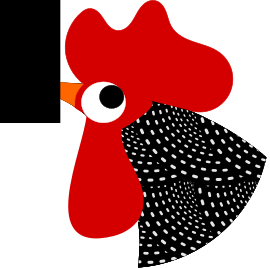
\includegraphics[width=#1]{../artwork/smallpantade}}
\newcommand{\warnsign}[1]{\includegraphics[width=#1]{../artwork/Ambox_warning_pn}}

\newcommand{\mcbpplevel}[1]{
\switch[#1=]
\case{1}
\case{2} \hspace{0.6cm} \coqhead{0.6cm}
\case{3} \coqhead{0.6cm} \coqhead{0.6cm}
\otherwise Please use \textbackslash mcbLEVEL
\endswitch
}
\newcommand{\mcbpptxtlevel}[1]{
\switch[#1=]
\case{1}
\case{2} $(\star)$
\case{3} $(\star\star)$
\otherwise Please use \textbackslash mcbLEVEL
\endswitch
}


\newcommand{\mcbvarreset}{
\mcbLEARN{Please use \textbackslash mcbLEARN}
\mcbREQUIRE{Please use \textbackslash mcbREQUIRE}
\mcbPROVIDE{Please use \textbackslash mcbPROVIDE}
\mcbNOTES{}
\mcbLEVEL{4}}

\newcommand{\mcbLEARN}[1]{\def\mcbvarLEARN{#1}}
\newcommand{\mcbREQUIRE}[1]{\def\mcbvarREQUIRE{#1}}
\newcommand{\mcbPROVIDE}[1]{\def\mcbvarPROVIDE{#1}}
\newcounter{mcbvarLEVEL}
\newcommand{\mcbLEVEL}[1]{\setcounter{mcbvarLEVEL}{#1}}
\newcommand{\mcbNOTES}[1]{\def\mcbvarNOTES{#1}}
\newcounter{mcbvarTMP}

\newcommand{\mcbsection}[1]{
\setcounter{mcbvarTMP}{1}
\ifthenelse{\equal{}{\mcbvarNOTES}}{\setcounter{mcbvarTMP}{0}}{}
\section[#1 \mcbpptxtlevel{\value{mcbvarLEVEL}}]{#1}
\smash{\raisebox{0.7cm}{\hspace{0.92\textwidth}\mcbpptxtlevel{\value{mcbvarLEVEL}}}}
%\marginnote{\small\begin{tabular}{p{3.8cm}}\hline
%\textbf{Learns} \mcbvarLEARN \\
%\textbf{Requires} \mcbvarREQUIRE \\
%\textbf{Provides} \mcbvarPROVIDE \\
%\textbf{Level} \arabic{mcbvarLEVEL} \\
%\switch[\value{mcbvarTMP}=]
%\case{0}
%\case{1} \textbf{Note} \mcbvarNOTES \\
%\endswitch
%\hline
%\end{tabular}\\~\\
%}
\mcbvarreset{}
}

\newcommand{\mcbsubsection}[1]{
\setcounter{mcbvarTMP}{1}
\ifthenelse{\equal{}{\mcbvarNOTES}}{\setcounter{mcbvarTMP}{0}}{}
\subsection[#1 \mcbpptxtlevel{\value{mcbvarLEVEL}}]{#1}
\smash{\raisebox{0.7cm}{\hspace{0.92\textwidth}\mcbpptxtlevel{\value{mcbvarLEVEL}}}}
%\marginnote{\small\begin{tabular}{p{3.8cm}}\hline
%\textbf{Learns} \mcbvarLEARN \\
%\textbf{Requires} \mcbvarREQUIRE \\
%\textbf{Provides} \mcbvarPROVIDE \\
%\textbf{Level} \arabic{mcbvarLEVEL} \\
%\switch[\value{mcbvarTMP}=]
%\case{0}
%\case{1} \textbf{Note} \mcbvarNOTES \\
%\endswitch
%\hline
%\end{tabular}\\~\\
%}
\mcbvarreset{}
}


\newcommand{\mcbsubsubsection}[1]{
\setcounter{mcbvarTMP}{1}
\ifthenelse{\equal{}{\mcbvarNOTES}}{\setcounter{mcbvarTMP}{0}}{}
\subsubsection[#1 \mcbpptxtlevel{\value{mcbvarLEVEL}}]{#1}
\smash{\raisebox{0.7cm}{\hspace{0.92\textwidth}\mcbpptxtlevel{\value{mcbvarLEVEL}}}}
%\marginnote{\small\begin{tabular}{p{3.8cm}}\hline
%\textbf{Learns} \mcbvarLEARN \\
%\textbf{Requires} \mcbvarREQUIRE \\
%\textbf{Provides} \mcbvarPROVIDE \\
%\textbf{Level} \arabic{mcbvarLEVEL} \\
%\switch[\value{mcbvarTMP}=]
%\case{0}
%\case{1} \textbf{Note} \mcbvarNOTES \\
%\endswitch
%\hline
%\end{tabular}\\~\\
%}
\mcbvarreset{}
}
\mcbvarreset{}

\newbox{\devnull}
\NewEnviron{coqdef}[1]{}

\newcommand{\coqrun}[2]{}

\newtcblisting[auto counter]{coq}[2]{
	listing engine=listings,
	listing options={numbers=left,numberstyle=\tiny,
	                 aboveskip=0mm,belowskip=0mm,
		         xrightmargin=0mm,xleftmargin=0mm},
	%on line,
	before={\noindent},
	after={\hfill},
	listing only,
	fonttitle=\small\sffamily,%\bfseries,
	boxrule=0.2mm,top=1mm,bottom=1mm,
	#2
}
\newtcblisting{coqout}[2]{
	listing engine=listings,
	listing options={aboveskip=0mm,belowskip=0mm,
	                 xrightmargin=0mm,xleftmargin=0mm},
	%on line,
	before={\noindent},
	after={\hfill},
	listing only,
	fonttitle=\small\sffamily,%\bfseries,
	boxrule=0.2mm,top=1mm,bottom=1mm,
	#2
}

\newcommand{\Coq}{\textsc{Coq}}
\newcommand{\mcbCIC}{Calculus of Inductive Constructions}


\makeindex[name=ssr,title=Index: Ssreflect tactics,intoc]
\makeindex[name=coq,title=Index: Coq terms,intoc]
\makeindex[name=vernac,title=Index: Coq commands,intoc]

\title{The Book}
\author{Assia, Enrico, \ldots (you are welcome)}

\begin{document}
\maketitle

% \setcounter{chapter}{-2}
\chapter{Conventions}

Words:\\
\begin{tabular}{ll}
used & unused \\\hline
implicit argument, place holder & existential/meta variable \\
language of canonical structures & hints \\
declarative program & logic program \\
type inference & pretyping, elaboration \\
\end{tabular}



\setcounter{chapter}{-1}
\chapter{The essence of math comp}

\section{challenges faced and tools adopted}
(tools in a broad sense, the logic is a tool, coq is a tool, the plugin
is a tool, the ssr style is a tool,...)

Challenges:
\begin{itemize}
\item large body (scale up), make proofs small and robust.
	We need to say that we do use "deterministic automation".
	Use Laurent's data on de bruijn factor.
\item model the use of math notations, their role in proofs, model proofs (also
	it is about reasoning, not just computations). Another way to say that
	is: model Bourbaki (rationalization of Math via structure/interfaces)
	but not the first book (set theory) that is replaced by CIC (link with
	section computational thinking).
\end{itemize}

We build on Coq and an extension.  The main tools follow (in random order):

\section{Computational Thinking}\label{ch:compthink}

This section should motive the activity of formalizing mathematics
with the {\bf Coq} proof assistant, emphasizing its computing skills,
and as opposed to other foundations like HOL. However the challenge is
to keep mathematicians as the privileged target, while motivating the
ssr approach to a CS oriented reader.

See \verb+../coq/ch0.v+.

Aim of the chapter:
\begin{itemize}
\item should sound natural and easy to a CS person (but with the ssr twist)
\item should sound different but well motivated to a Coq user (do show, maybe in
  the exercises, that leqn is 100 times better than "Inductive le").  Try to
  reproduce the shock we had the first time we used Boolean predicates.  It may
  help to compare, in the *advanced* section, the approach with the standard
  one, so that one sees two proof scripts in the same page.
\end{itemize}

\section{logic programming ... type inference}
to model proof search, give a meaning to notations, teach coq the
work an informed reader does (contextualizing otherwise ambiguous
notations, knowledge of interface/instance of algebraic structures).

relation with proof search: no "blind" proof search (easy, ad-hoc, pervasive
v.s. advanced, generalistic, potentially expensive and unstable).

\section{automation in tactics}
the main points:
\begin{itemize}
\item 1/3 is rewrite, term selection/search (one does not need to reach a sub
	formula as a goal in order to make progress for example, no monkey
	puzzle as in GG terminology).
\item Create a formula without writing it: some advanced forms of forward
	reasoning tactics to deal with symmetries, generalizations (boils down
	to syntesize the cut formula out of the minimum possible user input, as
	in a text where one says "similarly to that, we can also prove that".
	(this is not very pervasive, dunno if it is worth putting it here in
	this chapter).  Also elim does that. (technically also rewrite, but we
	may want to separate things)
\end{itemize}
This section is were one talks about the plugin, and some of the main design
points of tactics: compositional (a language, not a list of commands),
predictable (documented!!!), finally compact (symbols for uninteresting steps).

\section{discipline}
MAKE an howto out of that.
Maybe one should also add a few notes on the style in scripts? like:
\begin{itemize}
\item you must be able to model (at least) 1 proof step in a sentence (line),
  e.g. "rewrite preparegoal dostep ?cleanup."
\item uninteresting/recurrent lemmas/steps should be small (short names, easy to
  gray out)
\item lemma statements are designed, not just written, having in mind their use
      (forward, backward, implicit argumets, arguments order)
      and the class of trivial hypotheses since an extra hyp that is proable
      triviality (via //, hint resolve, cnaonical) is for free. E.g.
      "x \\is a toto", "0 <= n", ...
\item also not every possible lemma, but a few that combine well
\item proofs/definitions are reworked many times, why (understand recurrent
  proof schemas, compact, factor, make more stable/robust) and what is needed
  (like meaningful names, clear structure)
\end{itemize}

\section{trivial=implicit (for a trained mathematician)}
The idea is to try to identify what is trivial (mathematically speaking)
and be sure you can model it as such:
\begin{itemize}
\item (level basic) make explicit the trivialities of each theory (what one
	expects to be proved by //). 
\item (level advanced) when you do new stuff, you must decide what is
	trivial/implicitly proved.
\item (hard) which technique to make Coq prove it automatically (hint resolve,
	canon, comput... in the type)
\end{itemize}

This may also be another way present the whole chapter

\mantra{(basic) if you see toto=false you should perform the case analysys via fooP}


\tableofcontents{}

\part{Definitions and proofs}


\chapter{Computational definitions \\ The syntax of terms \\[2ex]\Large\itshape Defining concepts by writing programs} 

Find a more catchy title? The motivation is: how to define things:
objects, operations, (boolean) relations.

Theoretical content:
\begin{itemize}
\item Functions with simple types ($\lambda$, $\rightarrow$): functions are the primitive concept
\item Inductive {\bf datas}
\item Programs by case analysis and recursion
\item Compute (beta, delta, iota) example of beta (that helps later on to explain a predicate for elim principles
\item Polymorphic datatypes (introduce $\Pi$, and its \Coq{} notation
  \C{forall}, for quantification over datatypes only)
\item Everyone has a type : \C{0 : nat : Type : Type}, types avoid confusion
\end{itemize}
This is more or less a standard introduction to (a flavor of)
functional programming, with two possible difficulties:
\begin{itemize}
\item Be precise but not too technical (e.g. on inductive types)
\item Find a line of speech which does not bore/discourage
  mathematicians.
\item Somehow the syntax of (this fragment of the) terms should made
  be clear and precise.
\end{itemize}

\Coq{} commands and features:
\begin{itemize}
\item Implicit arguments (only to go from system F to ML), \C{@}
\item Sections and its discharging, implicit types
\end{itemize}

Comparison with other approaches:
\begin{itemize}
\item Compare an axiomatic, equational presentation of arithmetic to
  its formalization as an inductive type with functions that
  compute. At this stage, where we do not have conversion yet, we
  cannot say much about the proofs and may be just point out that
  computation in \Coq{} is geared toward the reduction of functional
  programs.
\end{itemize}

\Coq{} types introduced:
\begin{itemize}
\item \C{bool, nat, seq, option, prod}
\end{itemize}

Programs presented in detailed examples/exercises:
\begin{itemize}
\item Elementary programs on \C{option}: \C{odflt, obind,}\dots
\item Elementary programs on \C{seq} (without the \C{eqType}):
  \C{size, map, iota,...}
\item Comparison functions on \C{bool, nat}
\item Comparison functions on containers, taking the comparison
  function on the type of stored elements in argument (mind the
  higher-order)
\item Boolean connectives, arithmetic operations on \C{nat}
\item Euclidean division, computation of prime factors, examples from
  elementary number theory
\item Examples of G{\"o}del-style encoding from the {\tt choice.v} library.
\end{itemize}
If possible give a few context to the exercises, in order not to bore
the reader not familiar with programming. For instance do not say that
you encode sequences of nats in nats but give a few hints about the
use of G{\"o}del encoding.


\Chapter{What is a (Coq) proof\\The syntax of proofs}{Constructing proofs as programs}

% From calculability to proofs, hence the CC, and the fact that
% reasoning principles without a computational content become axioms.
%
% This is a non technical chapter and message should be:
% \begin{itemize}
% \item instantiation of a universal statement is application (also the pair)
% \item Excluded middle is not available by default (choice?)
% \item Conversion as a pervasive indistinguishably, what inside
%   (beta, definition unfolding,...)
% \item Dependent types: eq, sigma (which example?)
% \end{itemize}
%
% One options is: avoid relating type theory and other logics. We say:
% we have a formal game where the basic elements are programs/functions
% that come with types to avoid confusion. full stop. (no relation with
% proof theory, set theory). maybe mention that roots are in calculability (hence
% the choice to pick functions as primitive and not sets). This is lucky because
% (computable) functions are today executable by a computer.  Still not all
% concepts are "computable" hence some principles are problematic: EM,.... we
% mainly stay in the lucky fragment (again no propaganda on intuitionistic logic,
% constructive math; just a mention).
%

running topic: statements and their proofs. This chapter provides a gentle
introduction to the implicative fragment of the logic and to the
interactive construction of formal proofs. The reference to
Curry-Howard should come as late as possible. It should indeed be
possible to present a substantial amount of example and intuitions
before explaining this. Specially if we carefully use the automated
introduction of variables bound before the semi-column. At the tactic
level, we should be able to avoid the need for Curry Howard related
constructions like \C{apply: (H x)} in the first part of the chapter.

\begin{itemize}
\item \C{Prop} as the type of statements
\item forall-lambda, predicates as functions to Prop.  The difference with the forall in the previous chapter is that the type the var ranges in is not "Type" but a data type like nat.
\item examples with implicative predicate logic, modus ponens
\item definition = lemma (proofs of implications are lambdas-app)
\item tactics to generate the terms in a less pedestrian way (move, apply)
\item if one calls Show Proof in the middle he sees one is building
	the proof term incrementally, as one draws a proof tree (in CH style)
\end{itemize}

Now we make the point of Qed, the kernel checks the term produced via
tactics (or hand-written).

Examples of predicates: equality
\begin{itemize}
\item not to talk about indexes of inductive families we introduce eq as
	an axiom and refl as another axiom to prove eq and we insist on
	conversion
\item examples, among which a beta expansion (to help later on with elimination)
\item now, what are the proofs of an equality? maybe we start with rewrite
\item examples are symmetry, transitivity
\item then we give the elimination principle as an axiom, and explain the
	work rewrite does in synthesizing the predicate
\item the job of rewrite is not trivial nor un-ambiguous: to drive the synthesis show occurrence selection (later on we see the same problem for elim)
\item other exercise on other eq related "commands" like discriminate, injection arrows, congr.
\end{itemize}

Showing universal properties on inductive data
\begin{itemize}
\item first enouce some lemmas on concrete examples, like not true = false,
	then try to say "froall b : bool, ...".
\item first on enumerated types (bool) via case
\item them on nat via case and elim
\item then show the proof term as an application of nat-rect, again the problem
	is to write down P and elim does that.
\item here an additional problem: loading the goal before using it to generate P
\end{itemize}

We should manage to prove stuff on the concepts defined in chapter 1,
notably \C{odd(a+b) = xor (odd a) (odd b)}.  But before you need lemmas
on "odd (S x) = not (odd x)", to make the point that the proof is trivial with
a library that has all the needed facts.  Also the base case goes away by ssr (in general spell out where the computation saves work).

Comparison with other approaches:
\begin{itemize}
\item Compare an axiomatic, equational presentation of arithmetic to
  its formalization as an inductive type with functions that
  compute.
\end{itemize}


Another example is set-nth of rcons as done by Florent Hivert, that has not
developed the theory of set-nth with cat, and hence messes up the proof
that gets shorter if one does the homework.

Another example could be a proof that requires the induction principle
on nat that (strong/course of values induction).

A maybe good example that forces you to do patterns or occ numbers and explain
that 2  contains syntactically 0 is the proof that code/decode cancel (in
choice).

We lack example with a mathematical interest, maybe arithmetic is sufficient like binomial.v.

We need also /= and hence Arguments simple never (and we try to omit nosimpl).
Maybe we should document that nosimpl has been superseeded by
the option of Arguments in the manual.
Let say that controlling reduction is an important topic when you
do ssr style.

In this chapter we present several features of the proof language, but it it is
not about the proof language itself (reference manual). What one adds to the
reference manual here is an example of usage in the right context of the
commands.  E.g. we give an hint of what patterns do (rewrite) but we don't
discuss all the matching discipline... nor the most advanced syntaxes)

\section{Equality, proofs of equality}

Coq comes with an equality predicate, that we see as axiomatic for the
moment (in this section). It is called \C{eq} and has an infix
notation \C{=}. Can we avoid talking about \C{Prop} at this stage?

\begin{coq}{}
Check eq  (* : forall A : Type, A -> A -> Prop *)
Notation "x = y" := eq _ x y.
\end{coq}

Now we can state equalities and prove some of them, showing along the way
that equality is modulo computation (or is it too early?). This could
be our first interactive proof script:

\begin{coq}{}
Lemma toto1 : 3 + 2 = 5. by []. Qed.
\end{coq}

and we comment the different parts of this sentence.  Other examples
of proofs, this time by rewriting (assumptions stated
outside of the goal). Soft intro to pattern matching of \C{(_ + _)}

Examples could be to prove trans/symmetry of eq via rewrite (no proof terms
here).

Show \C{rewrite -H}, plus the idea that one may want to select
occurrences (with simple patterns).

Proofs can be done by case analysis, like brute force
proofs of boolean tautologies: Start with simple tests, analogues of
the example on numbers.

\begin{coq}{}
Lemma l1 : true && false = false. by []. Qed.
Lemma l2 : false && false = false. by []. Qed.
\end{coq}

An other example on nats:

\begin{coq}{}
Lemma eqn_refl (x : nat) : eqn x x = true.
\end{coq}

Then show that we also want

\begin{coq}{}
Lemma andbF b : b && false = false
\end{coq}

and hence easoning by cases. Now the analogue for nat:

\begin{coq}{}
Lemma addnC x : x + 0 = x.
\end{coq}

requires induction.

We also need ways to control computations of symbolic stuff,
Arguments simpl, or write the equations or \C{/=} and similar.


 Can we already show how \C{= true} can be used
in programs? We can also introduce basic proofs by recurrence like
\C{addnC}.

At which moment do we start using the coercion \C{is_true}? Anyhow, it
should be in this chapter.

May be should we say rather early that rewriting under binders is not
allowed by the system.
\section{Implication, universal quantification}

\subsection{Implication}
Here we need to introduce \C{Prop}, which is like \C{Type} but for provable
things. compare the source and target of arrows.

\begin{coq}{}
Inductive |*list*| (A : Type) : Type :=
    nil : list A | cons : A -> list A -> list A

list: Type -> Type

Definition |*is_equal_to_2*| (x : nat) : x = 2.

is_equal_to_2 : nat -> Prop
\end{coq}

Note: impredicativity is out of topic here.

We then show more examples of interactive proof scripts, introducing
(simple) \C{apply} and introduction steps. More examples of proofs by
induction?

\subsection{Universal quantification}

In fact all the statements that we have proved so far with parameters
are universally quantified statements. They use the same \C{forall} as
the one we saw on types.

\begin{coq}{}
nil   : forall A : Type, (seq A : Type)
andbF : forall b : bool, (b && false = b : Prop)
\end{coq}

Show the \C{move} tactic. Is this the place were we start talking
about CH? If so this is were we put:

Implication is arrow, Lemma = Definition.
Curry-Howard (terms are proofs)

\begin{coq}{}
Variable A : Prop.
Definition toto : A -> A := fun x => x.
Lemma  toto : A -> A.
 Proof.
  move => x.
  Show Proof.
  apply: x.
 Qed.
\end{coq}

Note : \C{toto :  A -> A : Prop}
discuss interactive proof construction, other example with a real
apply that open subgoals.

In CH style we see a proof, where lambdas/apply work too (same tactics)

Specialization of an quantified lemma via application (maybe also
\C{move/(_ x) in H}).
Soft intro of the work of unification (FO) during application (infer
arguments of conclusion's predicate symbol \C{prime _}).

We should also display her  HO "predicators": commutative.  Discuss
order of quantification in transitive and similar, naming conventions

\section{Curry-Howard for equality proofs}

\subsection{proof term for rewrite (CH)}

There are also proof terms for equality proofs (show \C{refl})
The work rewrite does is non trivial (infer P)

\begin{coq}{}
Check eq_rect (* : forall P : nat -> Prop, .... forall n, P n *)
\end{coq}

Write a proof term by hand.
(note that it works because of beta being part of conversion).
See that rewrite does the verbose part for you (infer P).

An example of ambiguous P from above, driving rewrite means driving the
synthesis of P.

\subsection{other eq related tactics}

Congr, injection \C{[= ]}, discriminate (//), \C{->}.


\subsection{proof term for induction}

Again show that it boils down to infer P


\subsection{proofs by induction in their generality}

Show that even for commutativity of addition one needs to
"load the goal" (or to help synthesize a more general P).


\section{Exercises (explained)}

xor-odd, then cancel encode decode, or something on primes.

Take the occasion to present last/first, bullets, by, syntaxes for
\C{=> [|IH x xs]} after a case.

\Chapter{Type Theory}{The Curry-Howard correspondence}
\label{ch:ttch}

The authors made the deliberate choice to postpone the presentation of
the mathematical foundations of the \Coq{} system and the formal
definition of its language. Instead, the previous chapters have
insisted on the definition of (typed) programs and on the way these
programs can be used to decribe computable functions and decidable
predicates. This take on calculations is indeed both at the core of
the type theory underlying \Coq{} and one of the crucial ingredients
to the methodology basing the \mcbMC{} library. The present chapter is
devoted to a more in-depth presentation of these mathematical
presentation, alhough an exhaustive description shall remain out of
the scope of the present book. The interested reader can refer to more
specialized references like~\cite{hottbook} or \cite{ttfp}, or the
shorter survey in the Handbook of Automated
Reasoning~\cite[Volume 2, Chapter 18]{handbook-ar}.

.



% By now the informed reader is likely to wonder when the authors of the book
% will eventually mention the mathematical foundation of \Coq{},
% % a variant of type theory called \mcbCIC{},
% and
% in particular explain the Curry-Howard isomorphism.  Indeed this text departs
% from the standard presentation of \Coq{}, that typically starts by
% explaining the logic and showing how standard connectives like
% conjunction or disjunction are defined in term of inductive types.

% We made a deliberate choice to put forward the programming aspects of
% type theory and how programs can be used both to express computable functions
% and decidable predicates or boolean connectives.
% Indeed this formalization choice is one of the main ingredients of the \mcbMC{}
% library.  The computational behavior of programs is at the core of
% type theory.  The fact that a function computes to a value requires no
% proof: 5 and 2+3 are indistinguishable from a logical standpoint.
% This fact provided a powerful form of automation, and as we will
% see later will also ease the construction of sub types.

% It is finally time to provide a minimal presentation of the statements as types
% correspondence.  The universe of boolean predicates is limited: one
% cannot for example express a general $\exists$ quantification, and also the
% status of the $\forall$ quantification has been so far never really explained.
% This presentation is far from being exhaustive, the interested reader can find
% a modern presentation of type theory in \cite{hottbook}.

\section{Connectives}

\subsection{Primitive types and terms formers}\label{sec:chi}

In type theory we say that \emph{logical statements} correspond to
\emph{types} and that \emph{proofs} correspond to \emph{programs}.

The simplest example one could think of is the formal statement saying that
a proposition $A$ implies itself, namely $A \rightarrow A$.  If one reads
the implication symbol $\to$ as the type of functions, the statements reads
as a function from $A$ to $A$.  A program with that type would be
\C{(fun x : A => x)}.  Such program takes in input a term $x$ of
type $A$, that we here see as a proof of $A$, and returns it, i.e. it
produces in output a proof of $A$.  We say that such program is a
proof of $A \rightarrow A$.

What is striking here is that the same class of terms represents both programs
and proofs, for example the identity function of natural numbers has the very
same shape of the proof we've just seen.  So we are left with only two
concepts, types and terms, playing a double role.  We now see how types and
terms can be formed.

Regarding types, the primitive type formers we have seen are the function space
$\to$, also logical implication, and the universal quantification
$\forall$, used to describe polymorphic function as well as parametric lemmas
(like induction principles).
Standard logical rules describing how one can prove formulas involving these
connectives are:

\begin{center}
\AxiomC{$A$}
\noLine
\UnaryInfC{$\vdots$}
\noLine
\UnaryInfC{$B$}
\RightLabel{$\to_I$}
\UnaryInfC{$A \to B$}
\DisplayProof
\hspace{1cm}
\AxiomC{$B$}
\RightLabel{$\forall_I$ ($x$ fresh)}
\UnaryInfC{$\forall x, B$}
\DisplayProof
\end{center}

The former reads: to prove $A \to B$ one can prove $B$ under the
assumption $A$.  The latter: to prove $\forall x,B$ one can prove $B$
assuming that $x$ is fresh.  We annotate such rules with the terms
corresponding to these proof rules.

\begin{center}
\AxiomC{\C{x : }$~A$}
\noLine
\UnaryInfC{$\vdots$}
\noLine
\UnaryInfC{\C{b : }$~B$}
\RightLabel{$\to_I$}
\UnaryInfC{\C{(fun x : A => b) : }$~A \to B$}
\DisplayProof
\hspace{1cm}
\AxiomC{\C{b : }$~B$}
\RightLabel{$\forall_I$}
\UnaryInfC{\C{(fun x : A => b) : }$~\forall x, B$}
\DisplayProof
\end{center}

The anonymous function constructor \C{(fun .. => ..)} serves as a proof
for both rules: the term \C{b} is in both cases a proof of $B$.  The only
difference is that $x$ is only allowed to occur in $B$ in the second rule.
Said otherwise in type theory $\to$ is a special case of $\forall$ where
the bound variable does not occur in the quantified formula.
For example
there is no semantic difference between \C{(nat -> bool)} and
\C{(forall x : nat, bool)}.

Logical connectives come with elimination rules, in particular

\begin{center}
\AxiomC{$A \to B$}
\AxiomC{$A$}
\RightLabel{$\to_E$}
\BinaryInfC{$B$}
\DisplayProof
\hspace{1cm}
\AxiomC{$\forall x, B$}
\RightLabel{$\forall_E$ ($t$ a term)}
\UnaryInfC{$B[t/x]$}
\DisplayProof
\end{center}

Function application serves as a proof for both rules.

\begin{center}
\AxiomC{\C{f : }$~A \to B$}
\AxiomC{\C{t : }$~A$}
\RightLabel{$\to_E$}
\BinaryInfC{\C{(f t) :}$~B$}
\DisplayProof
\hspace{1cm}
\AxiomC{\C{f : }$~\forall x : A, B$}
\AxiomC{\C{t : }$~A$}
\RightLabel{$\forall_E$}
\BinaryInfC{\C{(f t) : }$~B[t/x]$}
\DisplayProof
\end{center}

The programs as proofs correspondence has a visible impact in the proofs
part of the \mcbMC{} library.  In particular quantified lemmas, being programs,
can be instantiated by simply passing arguments to them.  Exactly as one can
pass \C{3} to \C{addn} and obtain \C{(addn 3)}, the function adding three, one
can ``pass'' \C{3} to the lemma \C{addnC} and obtain a proof of the statement
\C{(forall y, 3 + y = y + 3)}.  Remark that the argument passed to \C{addnC}
shows up in the type of the resulting term \C{(addnC 3)}:  the type of the
\C{addnC} program depends on the value the program is applied to.  That is the
difference between the \emph{dependent function space} ($\forall$)
and the standard function space ($\to$).
\index[concept]{dependent function space}

\mantra{Lemma names can be used as functions and you can pass to them arguments.
For example
\C{(addnC 3)} is a proof that \C{(forall y, 3 + y = y + 3)} and
\C{(prime_gt0 p_pr)} is a proof that \C{(0 < p)} whenever
\C{(p_pr : prime p)}.}

Finally note that the $\forall$ quantification specifies the type of the bound
variable, and that the $\forall_E$ checks the term $t$ has the ``right type'',
otherwise we get a type error.  What is particularly relevant to the \mcbMC{}
library is the notion of right type, or how types are compared.  Indeed
the $\to_E$ rule (and also the $\forall_E$) should be written as follows.

\begin{center}
\AxiomC{\C{f : }$~A \to B$}
\AxiomC{\C{a : }$~A'$}
\AxiomC{$A \equiv A'$}
\RightLabel{$\to_E$}
\TrinaryInfC{\C{(f a) :}$~B$}
\DisplayProof
\end{center}

We say that $A$ and $A'$ are checked for \emph{convertibility} ($\equiv$),
i.e. if they are equal up to computation.  As a consequence
the term \C{(isT : true)} is a perfectly valid proof of
\C{(0 < n.+1)}, as well as \C{(odd 7)} or \C{(prime 27)}
and can be passed to a lemma expecting any of these.
\index[coq]{\C{isT}}
\index[concept]{convertibility}

\subsection{Inductive types}\label{ssec:indtypes}

In the previous chapters we used many data types already.  For example we have
seen the type \C{nat} and its constructors \C{O} and \C{S}.  Through the looking
glasses of the Curry-Howard correspondence \C{O}, being a term of type \C{nat}
can represent a ``proof'' of \C{nat}.  For data types we prefer to say
\emph{inhabited} rather than \emph{proved}, but there is no real difference.

Inductive ``data'' types can be used to represent logical connectives, in
particular the ones we miss so far, like the existential quantifier.

\begin{center}
\AxiomC{$A$} \AxiomC{$B$}
\RightLabel{$\wedge_I$}
\BinaryInfC{$A \wedge B$}
\DisplayProof
\hspace{1cm}
\AxiomC{$A \wedge B$}
\RightLabel{$\wedge_E$ (left)}
\UnaryInfC{$A$}
\DisplayProof
\end{center}

The first rule reads: to prove $A \wedge B$ one needs to prove both
$A$ and $B$.  The latter lets one prove $A$ whenever one can prove
the stronger statement $A \wedge B$.

In \Coq{} such connective can be characterized by the following
inductive definition.

\begin{coq}{name=And}{}
Inductive and (A B : Prop) : Prop := conj (pa : A) (pb : B).
Notation "A /\ B" := (and A B).
\end{coq}
\index[vernac]{\C{Inductive}}

Remark that the ``data'' type \C{and} is tagged as \C{Prop}, i.e.  we declare
the intention to use it as a logical connective rather than a data type.  The
only constructor \C{conj} that can be used to inhabit \C{and} takes two
arguments, a proof of \C{A} and a proof of \C{B}, faithfully modelling the
logical rule \C{$\wedge_I$}.  Note that \C{A} and \C{B} are parameters of the
inductive definition, similarly to the definition of polymorphic lists
or pairs.

It is worth to note that the definition of the pair data type,
Exercise~\ref{ex:pair}, is almost identical to the one of \C{and}.

\begin{coq}{}{}
Inductive prod (A B : Type) := pair (a : A) (b : B).
\end{coq}
The striking similarity witnesses how programs (and data) are used in \Coq{}
to represent proofs.

Pattern matching provides a way to express the elimination rule for
conjunction as follows:

\begin{coq}{name=Ande1}{}
Definition proj1 A B (p : A /\ B) : A :=
  match p with conj a _ => a end.
\end{coq}
\index[coq]{\C{conj}}

Now recall the similarity between $\to$ and $\forall$, where the former is the
simple, non dependent, case of the latter.  If we check the type of
the \C{conj} constructor

\begin{coq}{name=Ande1}{width=4cm}
About conj.
\end{coq}
\begin{coqout}{}{width=8cm}
conj: forall A B : Prop, A -> B -> A /\ B
\end{coqout}
we may wonder what happens if the type of the second argument (i.e. \C{B}) is
made dependent on the value of the first argument (of type \C{A}).
What we obtain is the inductive definition corresponding to the
existential quantification.

\begin{coq}{name=Ande1}{}
Inductive ex (A : Type) (P : A -> Prop) : Prop :=
  ex_intro (x : A) (p : P x).
Notation "'exists' x : A , p" := (ex A (fun x : A => p)).
\end{coq}
\index[coq]{\C{ex_intro}}

The \C{ex\_intro} constructor is the only mean to prove a statement like
\C{(exists n, prime n)}.  In such case the first argument would be a number
\C{n} of type \C{nat} while the second argument would be a proof \C{p} of type
\C{(prime n)}.  The \C{ex} inductive definition is again pretty similar to the
pair, but note that the type of the second component depends on the value of
the first one.  Last note the parameter \C{P} that is a function
representing an arbitrary predicate over a term of
type \C{A}.  Hence \C{(P a)} is the instance of the predicate to \C{a}.  E.g.
the predicate of being an even prime number is expressed as
\C{(fun x : nat => ~~ (odd x) && prime x)}, and the statement expressing the
existence of such number is
\C{(ex nat (fun x : nat => ~~ (odd x) && prime x))}.

We quickly see the inductive definition of the disjunction \C{or}
and its two constructors \C{or\_introl} and \C{or\_intror}.

\begin{coq}{name=Or}{}
Inductive or (A B : Prop) : Prop := or_introl (a : A) | or_intror (b : B).
Notation "A \/ B" := (or A B).
\end{coq}

The elimination rule can again be expressed by pattern matching:

\begin{coq}{name=Or}{}
Definition or_ind (A B P : Prop)
  (aob : A \/ B) (pa : A -> P) (pb : B -> P) : P :=
  match aob with or_introl a => pa a | or_intror b => pb b end.
\end{coq}
\index[coq]{\C{or_introl}}
\index[coq]{\C{or_intror}}

The detail worth noting here is that the pattern match construct has two
branches, and each branch represents a distinct sub proof.  In this
case to prove \C{P} starting from \C{A \\/ B} one has to deal with all
cases: prove \C{P} under the assumption \C{A} and prove \C{P}
under the assumption \C{B}.

Usual constants and connectives as $\top$, $\bot$ and $\neg$
can be defined as follows.

\begin{coq}{name=TrueFalse}{}
Inductive True : Prop := I.
Inductive False : Prop := .
Definition not (A : Prop) := A -> False.
Notation "~ A" := (not A).
\end{coq}
\index[coq]{\C{True}}
\index[coq]{\C{False}}
\index[coq]{\C{I}}
\index[coq]{\C{not}}

Remark that to prove \C{True} one has simply to provide \C{I} that has no
arguments.  So proving \C{True} is trivial, and as a consequence eliminating it
provides little help (i.e. no extra knowledge is obtained by pattern matching
over \C{I}).  Conversely it is impossible to prove \C{False}, since it has no
constructor, and pattern matching on \C{False} can inhabit any type, since no
branch has to be provided.

\begin{coq}{name=exfalso}{}
Definition exfalso (P : Prop) (f : False) : P :=
  match f with end.  (* no constructors, no branches *)
\end{coq}

The only base predicate we are left to describe is equality.  The reason we
left it as the last one is that it has a tricky nature.  In particular
equality, as we have seen in the previous chapters, is an open notion
in the following sense.  Terms that compute to the same syntactic expression
are considered as equal, and this is true for any program the user may write.
Hence such notion of equality needs to be somewhat primitive, as
\C{match} and \C{fun} are.  One also expects such notion to come
with a substitutivity property: replacing equals by equals must be licit.

The way this internal notion is exposed is via the concept of index
on which an inductive family may vary.

\begin{coq}{name=Eq}{}
Inductive eq (A:Type) (x:A) : A -> Prop := erefl : eq A x x.
Notation "x = y" := (@eq _ x y).
\end{coq}
\index[concept]{equality}
\index[coq]{\C{erefl}}

This is the first time we see a function type after the \C{:} symbol
in an inductive type declaration.
The \C{eq} type constructor takes three arguments: a type \C{A} and
two terms of that type (the former is named \C{x}).
Hence one can write \C{(a = b)} whenever \C{a} and \C{b}
have the same type.
The \C{erefl} constructor takes no arguments, as \C{I}, but its type
annotation says it can be used to inhabit only the type \C{(x = x)}.
Hence one is able to prove \C{(a = b)} only when \C{a} and \C{b} are
equal up to computation (as in indistinguishable from a logical standpoint).
Conversely by eliminating a term
of type \C{(a = b)} one discovers that  \C{a} and \C{b} are
equal and \C{b} can be freely replaced by \C{a}.

\begin{coq}{name=EqInd}{}
Definition eq_ind A (P : A -> Prop) x (px : P x) y (e : x = y) : P y :=
  match e with erefl => px end.
\end{coq}

The notion of equality is one of the most intricate aspects of type
theory and an in depth study of it is out of the scope of this book.  The interested reader
finds an extensive study of this subject in~\cite{hottbook}.  Later in this
chapter we define and use other inductive families to take advantage
of the ``automatic'' substitution of the implicit equations we see here:
while \C{px} has type \C{(P x)} it is accepted as an
inhabitant of \C{(P y)} because inside the \C{match} the term \C{y}
is automatically replaced by \C{x}.

%%%%%%%%%%%%%%%%%%%%%%%%%%%%%%%%%%%%%%%%%%%%%%%%%%%%%%%%%%%%
\subsection{Proof commands}

Since proofs are just terms one could,
in principle, use no proof language and input directly proof terms.
Indeed this was the modus operandi in the pioneering work of
De Bruijn on Automath (automating mathematics) in the seventies~\cite{nederpelt-94}.
Of course a dedicated proof language can relief the user from
many tedious details.  The proof commands we have seen so far can all be
explained in terms of the proof terms they produce behind the scenes.
For example \C{case: n} provides a much more compact syntax
for \C{(match .. with .. end)} and it produces a
\C{match} expression with the right
shape by looking at the type of \C{n}.  If \C{n} is a natural number then there
are two branches, the one for the \C{S} constructor carries an argument of type
\C{nat}, the other one is for \C{0} and binds no additional term.
The \C{case:} tactic is general enough to work with any inductive data type
and inductive predicate.

The \C{apply:} tactic generates an application.  For example \C{apply: addnC}
generates the term \C{(addnC t1 t2)} by figuring out the correct values of
\C{t1} and \C{t2}, or opening new goals when this cannot be done, i.e.
if the lemma takes in input proofs, like \C{contraL}.

There is a list of proof commands that are shorthands for \C{apply:}
and is only worth mentioning here briefly. \C{split} proves a conjunction
by applying the \C{conj} constructor, \C{left} and \C{right} prove a
disjunction by applying \C{or\_introl} and \C{or\_intror} respectively.
\C{exist t} proves an existentially quantified formula by providing
the witness \C{t} and, later, a proof that \C{t} validates the predicate.
Finally \C{reflexivity} proves an equality by applying \C{erefl}.

%%%%%%%%%%%%%%%%%%%%%%%%%%%%%%%%
\section{Managing the proof context}
The only primitive constructor that remains without an associated proof command
is \C{(fun .. => ..)}.  Operationally what the $\to_I$ and
$\forall_I$ logical rule do is to introduce into the proof context a
new entry.  So far we either expressed this step at the beginning of proofs
by putting such items just after the name of the lemma being prover, or
just after a \C{case:} or \C{elim:} proof command.  The current section
expands on this subject covering the full management of the proof context.

%%%%%%%%%%%%%%%%%%%%%%%%%%%%%%%%%%%%%%%%%%%%%%%%%%%
\subsection{The stack model}
\index[concept]{goal stack model}

The presentation we gave so far of proof commands like \C{case: n => [|m]}
is oversimplified.  While \C{case} is indeed the proof command in
charge of performing case analysis the ``\C{: n}'' and ``\C{=> [|m]}''
parts are decorators to prepare the goal and post process the result of
the proof command.  These decorators deal with what we typically call
\emph{bookkeeping}: actions that are necessary in order to obtain readable and
robust proof scripts but that are too frequent to benefit from a move verbose
syntax.  Bookkeeping actions do convey a lot of information, like where
names are given to assumptions, but also let one deal with annoying details
using a compact, symbolic, language.  Note that all bookkeeping actions
correspond to regular, named, proof commands.  It is the use one makes of them
that may be twofold: a case analysis in the middle of a proof may start two
distinct lines of reasoning, and hence it is worth being noted explicitly with
the \C{case} word; conversely de-structuring a pair to obtain the two
components can hardly be a relevant step in a proof, so one may prefer to
perform such bookkeeping action with a symbolic, compact, notation
corresponding to the same \C{case} functionality.

%%%%%%%%%%%%%%%%%%%%%%%%%%%%%%%%%%%%%%%%%%%%%%%%%%%%%%%%%%%%%%%%%
\mcbLEVEL{1}
\mcbsubsubsection{Pulling from the stack}
\index[ssr]{\C{tactic => ..}}

Lets start with the post processing phase, called \emph{introduction pattern}.
The postfix ``\C{=> ...}'' syntax can be used in conjunction with any proof
command, and it performs a sequence of actions on the first goal assumption or
quantified variable.  With these looking glasses, the goal becomes a
\emph{stack}. Take for example this goal:

\begin{coqout}{name=Stack}{}
========================
forall xy, prime xy.1 -> odd xy.2 -> 2 < xy.2 + xy.1
\end{coqout}

Before accessing the assumption \C{(prime xy.1)} one has to name the
bound variable \C{xy}, exactly as one can only access a stack from its top.
The execution of \C{=> xy pr\_x odd\_y} is just the composition of
\C{=> xy} with \C{=> pr\_x} and finally \C{=> odd\_y}.  Each action
pulls out of the stack an item and names it.  The \C{move} proof
command does nothing,  we use it as a placeholder
for the postfix \C{=>} bookkeeping action.

\begin{coq}{}{width=7cm}
move=> xy pr_x odd_y
\end{coq}
\begin{coqout}{name=Stack1}{width=5cm}
 xy : nat * nat
 pr_x : prime xy.1
 odd_y : odd xy.2
========================
 2 < xy.2 + xy.1
\end{coqout}

Now, en passant, one would like to decompose \C{xy} into its first
and second component.  Instead of the verbose \C{=> xy; case: xy => x y}
one can use the symbolic notation \C{[]} to perform such action.

\begin{coq}{}{width=7cm}
move=> [x y] pr_x odd_y
\end{coq}
\begin{coqout}{name=Stack2}{width=5cm}
 x, y : nat
 pr_x : prime (x,y).1
 odd_y : odd (x,y).2
========================
 2 < (x,y).2 + (x,y).1
\end{coqout}
\index[ssr]{\C{tactic => ..}!\C{=> [ .. $\mid$ .. ]} (case)}

One can place the \C{/=} switch to force the system to reduce the formulas on
the stack, before introducing them in the context, and obtain:

\begin{coq}{}{width=7cm}
move=> [x y] /= pr_x odd_y
\end{coq}
\begin{coqout}{name=Stack2}{width=5cm}
 x, y : nat
 pr_x : prime x
 odd_y : odd y
========================
 2 < y + x
\end{coqout}

One can also process an assumption trough a lemma.  For example
\C{prime\_gt1} states \C{(prime p -> 1 < p)} for any \C{p}, and we can
use it as a function to obtain a proof of \C{(1 < x)}  from a proof
of \C{(prime x)}.

\begin{coq}{}{width=7cm}
move=> [x y] /= /prime_gt1-x_gt1 odd_y
\end{coq}
\begin{coqout}{name=Stack2}{width=5cm}
 x, y : nat
 x_gt1 : 1 < x
 odd_y : odd y
========================
 2 < y + x
\end{coqout}
\index[ssr]{\C{tactic => ..}!\C{=> /=} (simplification)}

The leading \C{/} makes \C{prime\_gt1} do as a function instead of
as a name to be assigned to the top of the stack.  The \C{-} has no effect but
to visually link the function and name assigned to its output.
Indeed \C{-} can be omitted.

One could also examine \C{y}: it can't be \C{0}, since it would contradict
the assumption saying that \C{y} is \C{odd}.

\begin{coq}{}{width=7cm}
move=> [x [//|y]] /= /prime_gt1-x_gt1.
\end{coq}
\begin{coqout}{name=Stack2}{width=5cm}
 x, y : nat
 x_gt1 : 1 < x
 ========================
 ~~ odd y -> 2 < y.+1 + x
\end{coqout}
\index[ssr]{\C{tactic => ..}!\C{=> /view} (view application)}
\index[ssr]{\C{tactic => ..}!\C{=> //} (close trivial goals)}

This time the destruction of \C{y} generates to cases, hence the \C{[ .. | .. ]}
syntax mentioning the two branches.  In the first one, when \C{y} is \C{0},
the \C{//} action solves the goal, by the same trivial means
of the \C{by []} terminator.  In the second branch we name \C{y} the
new variable.

Now, the fact that \C{y} is even is not needed to conclude, so we can discard it using the \C{\_} dummy name.

\begin{coq}{}{}
by move=> [x [//|y]] /= /prime_gt1-x_gt1 _; apply: ltn_addl x_gt1.
\end{coq}

The way to dispose an already named assumption is to mention
its name in curly braces, as \C{=> \{x_gt1\}}.
\index[ssr]{\C{tactic => ..}!\C{=> \{name\}} (disposal)}

We finally conclude with the \C{apply:} command that here we use
with two arguments: a function and its last argument.

\begin{coq}{}{width=4cm}
About ltn_addl.
\end{coq}
\begin{coqout}{}{width=8cm}
ltn_addl : forall m n p : nat, m < n -> m < p + n
\end{coqout}

\C{apply:} will fill in the blanks between the function (the lemma name)
and the argument provided.  Note that by passing \C{x\_gt1}, the
variable \C{m} picks the value \C{1}.  The conclusion of \C{ltn\_addl}
hence unifies with \C{(2 < y.+1 + x)} because both \C{+} and \C{<} are
defined as programs that compute: addition exposes a \C{.+1} by
reducing to \C{2 < (y+x).+1}, then \C{<}, or better the underlying
\C{<=}, eats a successor from both sides, leading to \C{1 < y + x}
that looks like the conclusion of the lemma we apply.

Here we have shown all possible actions one can perform in an intro
pattern, squeezing the entire proof into a single line.  This has
to be seen both as an opportunity and as a danger: one can easily
make a proof unreadable by performing too many actions in the bookkeeping
operator \C{=>}.  At the same time a trivial sub-proof like this one
should take no more than a line, and in that case one typically
sacrifices readability in favor of compactness: what would you learn by
reading a trivial proof?  Of course,
finding the right balance only comes with experience.

\gotcha{The case intro pattern \C{[..|..]} obeys an exception: when it is the first
item of an intro pattern, it does not perform a case analysis, but only branch
on the subgoals.%\footnote{not the status quo, but I prefer this exception to the current one}
Indeed in \C{case: n => [|m]} only one case analysis is performed.}


%%%%%%%%%%%%%%%%%%%%%%%%%%%%%%%%%%%%%%%%%%%%%%%%%%%%%%
\mcbLEVEL{1}
\mcbsubsubsection{Working on the stack}

The stack can also be used as a work place.  Indeed there is
no need to pull from the stack all items.  If we take the previous example

\begin{coqout}{name=Stack}{}
========================
forall xy, prime xy.1 -> odd xy.2 -> 2 < xy.2 + xy.1
\end{coqout}
and we stop just after applying the view, we end up is a valid state.

\begin{coq}{}{width=6cm}
move=> [x y] /= /prime_gt1.
\end{coq}
\begin{coqout}{name=Stack2}{width=6cm}
 x, y : nat
 ========================
 1 < x -> odd y -> 2 < y + x
\end{coqout}

One can also chain multiple views on the same stack item.

\begin{coq}{}{width=6cm}
move=> [x y] /= /prime_gt1/ltnW.
\end{coq}
\begin{coqout}{name=Stack2}{width=6cm}
 x, y : nat
 ========================
 0 < x -> odd y -> 2 < y + x
\end{coqout}
\index[ssr]{\C{tactic => ..}!\C{=> /view/view} (many views)}

Two other operations are available on the top stack item: specialization
and substitution.  Let's take the following conjecture.

\begin{coqout}{}{}
========================
(forall n, n * 2 = n + n) -> 6 = 3 + 3
\end{coqout}

The top stack item is a quantified assumption.  To specialize it to, say,
\C{3} one can write as follows:

\begin{coq}{}{width=4cm}
move=> /(_ 3).
\end{coq}
\begin{coqout}{}{width=8cm}
========================
3 * 2 = 3 + 3 -> 6 = 3 + 3
\end{coqout}
\index[ssr]{\C{tactic => ..}!\C{=> /(_ arg)} (specialization)}
The idea behind the notation is that when we apply a view to the top
stack item (we name it \C{top} here), as in \C{/v}, we are
forming the term \C{(v top)}, while
when we specialize the top assumption as in \C{/(_ x)} we form the
term \C{(top x)}.  The \C{_} is a place holder for the top item, and is
omitted in \C{/(view _)}.

When the top stack item is an equation one can substitute it using \C{<-}
and \C{->} for right-to-left and left-to-right respectively.

\begin{coq}{}{width=4cm}
move=> /(_ 3) <-.
\end{coq}
\begin{coqout}{}{width=8cm}
========================
6 = 3 * 2
\end{coqout}
\index[ssr]{\C{tactic => ..}!\C{=> ->} (rewriting L2R)}
\index[ssr]{\C{tactic => ..}!\C{=> <-} (rewriting R2L)}
In other words, the arrows are just a compact syntax for rewriting,
as in the \C{rewrite} tactic, with the top assumption.

%%%%%%%%%%%%%%%%%%%%%%%%%%%%%%%%%%%%%%%%%%%%%%%%%%%%%%%%%%%%%%%%%
\mcbLEVEL{1}
\mcbsubsubsection{Pushing to the stack}
\index[ssr]{\C{tactic : ..}}

We have seen how to pull items from the stack to the context.
Now let's see the so called \emph{discharging} operator \C{:}, performing
the converse operation.
Such operator decorates
proof commands as \C{move}, \C{case} and \C{elim}
 with actions to be performed before the command is actually run.

\gotcha{The colon symbol in \C{apply:} is not the discharging operator.
It is just a marker to distinguish the \C{apply:} tactic of
Ssreflect from the \C{apply} tactic of \Coq{}.
Indeed the two tactics, while
playing similar roles, behave very differently.}

Imagine we want to perform case analysis on \C{y} at this stage

\begin{coqout}{name=Stack2}{}
 x, y : nat
 x_gt1 : 1 < x
 odd_y : odd y
 ========================
 2 < y + x
\end{coqout}

The command \C{case: y} is equivalent to
\C{move: y; case.} where \C{move} once again is a place holder,
\C{: y} pushes onto the stack the \C{y} variable and \C{case}
operates on the top item of the stack.
%Pushing items on the stack is called \emph{discharging}.

Just before running \C{case} the goal looks like this:

\begin{coqout}{name=Stack2}{}
 x : nat
 x_gt1 : 1 < x
 odd_y : odd y
 ========================
 forall y, 2 < y + x
\end{coqout}

Unfortunately the binding for y is needed by the \C{odd\_y}
context item, so \C{move: y} fails.  One has to push on the stack
items in a valid order.  \C{move: y odd\_y} would push \C{odd\_y}
first, then \C{y}, leading to the valid goal

\begin{coqout}{name=Stack2}{}
 x : nat
 x_gt1 : 1 < x
 ========================
 forall y, odd y -> 2 < y + x
\end{coqout}
\index[ssr]{\C{tactic : ..}!\C{: term} (generalization)}

Via the execution of \C{case} one obtains:

\begin{coqout}{name=Stack2}{}
2 subgoals

  x : nat
  x_gt1 : 1 < x
  ========================
   odd 0 -> 2 < 0 + x

subgoal 2 is:
 forall n : nat, odd n.+1 -> 2 < n.+1 + x
\end{coqout}

An alternative to discharging \C{odd\_y} would be to clear it, i.e. purge it
from the context.  Listing context entry names inside curly braces has this
effect.  For example \C{case: y \{odd\_y\}}.
\index[ssr]{\C{tactic : ..}!\C{: \{name\}} (disposal)}

One can combine \C{:} and \C{=>} around a proof command, to first prepare the
goal for its execution and finally apply the necessary bookkeeping to the
result.  For example:

\begin{coq}{}{width=6cm}
case: y odd_y => [|y']
\end{coq}
\begin{coqout}{name=Stack2}{width=6cm}
2 subgoals

  x : nat
  x_gt1 : 1 < x
  ========================
   odd 0 -> 2 < 0 + x

subgoal 2 is:
 odd y'.+1 -> 2 < y'.+1 + x
\end{coqout}

At the left of the \C{:} operator one can also put a name for an
equation that links the term at the top of the stack before and
after the tactic execution.  \C{case E: y odd\_y => [|y']} leads to
the two sub goals:

\begin{coqout}{name=Stack2}{width=6cm}
 x, y : nat
 x_gt1 : 1 < x
 E : y = 0
============================
 odd 0 -> 2 < 0 + x
\end{coqout}
\begin{coqout}{name=Stack2}{width=6cm}
 x, y : nat
 x_gt1 : 1 < x
 y' : nat
 E : y = y'.+1
========================
 odd y'.+1 -> 2 < y'.+1 + x
\end{coqout}
\index[ssr]{\C{tactic : ..}!\C{name: term} (equation)}

Last, one can discharge the goal with any term, not
just variables occurring in it.  For example
``\C{move: (leqnn 7)}'' pushes on the stack
the additional assumption \C{(7 <= 7)}.  This
will come handy in section~\ref{sec:strongind}.

%%%%%%%%%%%%%%%%%%%%%%%%%%%%%%%%%%%%%%%%%%%%%%%%%%%%%%%%%%%%
\section{Inductive reasoning}\label{sec:indreason}

In chapter 1 we have seen how to build and use (call or destruct)
anonymous functions and data types.  All these
constructions have found a correspondence in the Curry-Howard correspondence.
The only missing piece is recursive programs.  For example
\C{addn} was written by recursion on its first argument, and is a
function taking in input two numbers and producing a third one.
We can write programs by recursion that take in input, among regular  data,
proofs and produce in output other proofs.  Let's look at the
induction principle for natural numbers trough the looking glasses of the
Curry-Howard isomorphism.

\begin{coq}{}{width=3.5cm}
About nat_ind.
\end{coq}
\begin{coqout}{}{width=9cm}
nat_ind : forall P : nat -> Prop,
  P 0 -> (forall n : nat, P n -> P n.+1) -> forall n : nat, P n
\end{coqout}
\C{nat\_ind} is a program that produces a proof of \C{(P n)} for any \C{n}
proviso a proof for the base case \C{(P 0)}, and a proof
of the inductive step \C{(forall n : nat, P n -> P n.+1)}.
Let's write such program by hand.

\begin{coq}{}{}
Fixpoint nat_ind (P : nat -> Prop)
  (p0 : P 0) (pS : forall n : nat, P n -> P n.+1) n : P n :=
  if n is m.+1 then
    let pm (* : P m *) := nat_ind P p0 pS m in
    pS m pm (* : P m.+1 *)
  else p0.
\end{coq}
\index[coq]{\C{nat\_ind}}

The \Coq{} system generates such program automatically
when the \C{nat} data type
is defined.  Recall that recursive functions are checked for termination:
trough the lenses of the proofs as programs correspondence this means
that the induction principle just coded is sound, i.e. based on a well
founded order relation.
\index[concept]{termination}
\index[concept]{consistency}

If non-terminating functions are not ruled out, it easy to inhabit
the \C{False} type, even if it lacks a proper constructor.

\begin{coq}{}{}
Fixpoint oops (n : nat) : False := oops n.
Check oops 3.  (* : False *)
\end{coq}
Of course \Coq{} rejects the definition of \C{oops}.  To avoid
loosing consistency, \Coq{} also enforces some restrictions on
inductive data types.  For example the declaration of \C{hidden}
is rejected.

\begin{coq}{}{}
Inductive hidden := Hide (f : hidden -> False).
Definition oops (hf : hidden) : False := let: Hide f := hf in f hf.
Check oops (Hide oops).  (* : False *)
\end{coq}
Note how \C{oops} calls itself, as in the previous example,
even if it is not a recursive function.
Such restriction, called
\emph{positivity condition}, is out of scope for this book.
The interested reader shall
refer to~\cite{Coq:manual}.
\index[concept]{positivity}

%%%%%%%%%%%%%%%%%%%%%%%%%%%%%%%%%%%%%%%%%%%%%%%%%%%
\mcbLEVEL{1}
\mcbsubsection{Strong induction}
\index[concept]{induction!strong}
\index[concept]{induction!curse of values}
\label{sec:strongind}

As an exercise we show how the \C{elim} tactic combined with the bookkeeping
operator \C{:} lets one perform, on the fly, a stronger variant of
induction called ``course of values''.

Claim: every amount of postage that is at least 12 cents
can be made from 4-cent and 5-cent stamps.  The proof in the inductive
step goes as follows.  There are obvious solutions for a postage between
12 and 15 cents, so we can assume it is at least 16 cents.  Since
the postage amount is at least 16, by using a 4-cents stamp we are back
at a postage amount that, by induction, can be obtained as claimed.\hfill$\square$

The tricky step is that we want to apply the induction hypothesis not
on $n-1$, as usual, but on $n-4$, since we know how to turn a
solution for a stamping amount problem $n$ to one for a problem of
size $n+4$ (by using a 4-cent stamp).
The induction hypothesis provided by \C{nat_ind}
is not strong enough.  However we can use the \C{:} operator
to load the goal before performing the induction.
\index[ssr]{\C{set name := term}}

\begin{coq}{}{}
Lemma stamps n : 12 <= n -> exists s4 s5, s4 * 4 + s5 * 5 = n.
Proof.
elim: n {-2}n (leqnn n) =>[|n IHn]; first by case.
do 12! [ case; first by [] ]. (* < 12c *)
case; first by exists 3, 0.   (* 12c = 3 * 4c *)
case; first by exists 2, 1.   (* 13c = 2 * 4c + 1 * 5c *)
case; first by exists 1, 2.   (* 14c = 1 * 4c + 2 * 5c *)
case; first by exists 0, 3.   (* 15c = 3 * 5c *)
move=> m'; set m := _.+1; move=> mn m11.
case: (IHn (m-4) _ isT) => [|s4 [s5 def_m4]].
  by rewrite leq_subLR (leq_trans mn) // addSnnS leq_addl.
by exists s4.+1, s5; rewrite mulSn -addnA def_m4 subnKC.
Qed.
\end{coq}

Just before the induction step the goal is the following one:

\begin{coq}{}{}
forall n m : nat,
  m <= n -> 11 < m -> exists s4 s5 : nat, s4 * 4 + s5 * 5 = m
\end{coq}
The corresponding induction hypothesis \C{IHn} is:

\begin{coq}{}{}
IHn : forall m : nat,
      m <= n ->
      11 < m -> exists s4 s5 : nat, s4 * 4 + s5 * 5 = m
\end{coq}
Such hypothesis is accessible for each \C{m} that is at least \C{12}
and smaller than \C{n}.

Loading the goal works as follows: first \C{(leqnn n)} is pushed on
the stack, then all occurrences of \C{n} but for the second one are
discharged obtaining

\begin{coq}{}{}
forall m : nat,
  m <= n -> 11 < m -> exists s4 s5 : nat, s4 * 4 + s5 * 5 = m
\end{coq}
Finally the last occurrence of \C{n} is discharged too so that induction is performed
on such quantified variable.

Lines 4, 9 and 10 deserve a few comments.  Line 4 repeats a tactic
12 times.  Line 9 uses the \C{set} proof command to name \C{m} a
term of the form \C{_.+1} where \C{_} is a wildcard. It names
\C{m} the term \C{m'.+16}.  Line 10 passes to the induction
hypothesis \C{(m-4)}, then a placeholder for a missing proof
of \C{(m-4 < n)}, finally a proof that \C{(11 < m-4)}.  The introduction
pattern in line 10 names \C{s4} and \C{s5} the quantities of
4-cents and 5-cents stamps needed to cover the amount of postage \C{(m-4)}.
\index[ssr]{\C{do n"!} (iteration)}


%%%%%%%%%%%%%%%%%%%%%%%%%%%%%%%%%%%%%%%%%%%%%%%%%%%%%
\mcbLEVEL{1}
\mcbsection{On the status of Axioms}
\label{sec:EM}

Not all valid reasoning principles can be represented by programs.
For example excluded middle can be proved by a program only when
the property is decidable, i.e. when we can write in \Coq{} a program
to \C{bool} that tests if the property holds or not.
Excluded middle, in its generality, can only be \emph{axiomatized},
i.e. assumed globally.

The \mcbMC{} library is axiom free.  This makes the library compatible
with as many axioms as possible.  Indeed not all combinations of well
known, consistent, axioms are consistent, so if a library picks
one it rules out another one.  Moreover the formalization style
we adopted systematically expresses all decidable properties
as boolean tests, hence one rarely notices that excluded middle
is ``missing''.

Sometimes axioms like excluded middle can be confined into ``boxes''
one can open only in contexts where they can be actually proved.
For example:

\begin{coq}{}{}
Definition classically P : Prop := forall b : bool, (P -> b) -> b.
Lemma classic_EM P : classically (decidable P).
Lemma classic_bind P Q :
  (P -> classically Q) -> classically P -> classically Q.
\end{coq}
\index[coq]{\C{classically}}
\index[coq]{\C{classically_EM}}
\index[coq]{\C{classically_bind}}
Here \C{classically} plays the role of a box, typically called \emph{monad}
in computer science, that one can only open when the goal is a boolean,
hence decidable, predicate.  Inside such box the excluded middle is
made available by combining \C{classic_EM} and \C{classic_bind}.
Nevertheless, when proving a statement that is not a boolean, like
\C{exists n, ...}, one cannot access assumptions in the \C{classically} box.

In other cases axioms can be avoided by rephrasing the mathematics
in a weaker setting.  A notable example in the \mcbMC{} library
is the construction of the real closure of an Archimedean
field~\cite{DBLP:conf/itp/Cohen12}.
%\marginnote{TODO Cyril: say more about RCF}


%%%%%%%%%%%%%%%%%%%%%%%%%%%%%%%%%%%%%%%%%%%%%%%%%%%%%
\mcbLEVEL{1}
\mcbsection{Terms, types, proofs: all in the same pot}

For a newcomer
a quite confusing feature of the \mcbCIC{} is that the same syntax
is shared among term, proofs, statements and data types.  In other words terms
can occur in types and types can occur in terms.  And of course terms and
types play the double role of proofs and statements respectively.
This is strictly related to the range the quantifications are allowed on,
and to the fact that they can be used to form types.
We have seen quantification on terms, like ``\C{ forall n : nat}'' and on types
like ``\C{ forall P : Prop}'' or ``\C{ forall T : Type}''.  The subtle difference
between the label \C{Prop} for propositions and \C{Type} for data types
is out of scope here, we consider them synonyms.

An excellent example of these quantification is the inductive type
modelling the existential quantification:

\begin{coq}{}{}
ex : forall A : Type, (A -> Prop) -> Prop.
ex_intro : forall A : Type, forall P : A -> Prop, forall a : A, P a -> ex A P.
\end{coq}

The \C{ex} type constructor is polymorphic in a type \C{A} and a predicate
on \C{A}.  Remark that also \C{seq} is polymorphic, but only in one argument
so the quantification can be non dependent: \C{(seq : Type -> Type)}.

In the constructor \C{ex_intro} the quantification on \C{P} also needs to be
dependent: first because it must build a term of type \C{(ex A P)} (that
mentions \C{P}); second because the last argument needs to be of a proof of
\C{P}, so its type must mention the predicate.  Again in the case of \C{seq}
the constructor \C{(cons : forall A, A -> seq A -> seq A)} needs no dependent
quantification on the head element, while here \C{a} needs to occur in
the type of the argument that follows it, since it must be a proof of
\C{(P a)}.

The \C{ forall } quantification is not only useful to form types that
play the role of propositions.  It can come handy to form data types
too.  In the second part of this book (section~\ref{sec:matrix})
we see how the matrix data type
and the type of its multiplication function benefit from it.

\begin{coq}{}{}
matrix : Type -> nat -> nat -> Type.
mulmx : forall R : Type, forall m n p : nat,
  matrix R m n -> matrix R n p -> matrix R m p.
\end{coq}

This time the data type of matrices exposes the size, and matrix multiplication
can be given a type that rules out incompatible matrices and also describes
the dimension of the resulting matrix in terms of the size of the input
ones.\footnote{In veritas, \C{mulmx} also needs to take in input operations to
add and multiply elements of \C{R}.  Such detail plays no role in the current
discussion.}
This last use of of the \C{ forall } quantifier is a classic example
of what is called a \emph{dependent type}: a data type depending on
data, two natural numbers here.
\index[concept]{dependent type}

Last, a quantification can also range on the proofs of a statement
so that one can talk about proofs.  Such capability finds a rare, but
crucial use in \mcbMC{} that we discuss in chapter~\ref{ch:sigmabool}.

\begin{coq}{name=hedberg}{}
Lemma bool_irrelevance (P Q : bool) : forall e1 e2 : P = Q, e1 = e2.
\end{coq}

%
%           nat -> nat a function, like pred
%forall x : nat, p n   a statement, n = n
%forall x : nat, T n   a rich data type constructor
%           Type -> Type  a poly data type constructor
%forall T : Type, F T     a polymorphic data type
%(bla : Prop) -> 'I_m
%
%Something possible but never? used in mcbmc is
%
%forall p : (bla : Prop), T p
%
%one may find
%
%forall i : 'I_k, T i
%
%but recall the proof part in i is irrelevant.
%
%
%

\Chapter{Boolean reflection}{ Advanced specifications}\label{ch:boolrefl}

% in addition to the photos:
% \begin{itemize}
% \item talk about /= in 2 as a decorator for elim on a list (since arithmetics is all loked with nosimpl).
% \item talk about nosimpl in 3.3, say that according to our experience simpl is not
% always a good idea hence nosimpl.
% \item good practice (3.3 or 3.4): state and prove the fixpoint unfolding/folding equations.
% \end{itemize}



%\section{Motivations}

At this stage, we are in presence of one of the main issues in the
representation of mathematics in a formal language: very often,
several datastructures can be used to represent a same mathematical
definition or statement. But this choice may have a significant impact
on the upcoming layers of formalized theories. We have seen so far two
ways of expressing logical statements: using boolean predicates and
truth values on one hand, and using logical connectives and the
\C{Prop} sort on the other. For instance, in order to define the
predicate ``the sequence \C{s} has at least one element satisfying the
(boolean) predicate \C{a}'', we can either use a boolean predicate:

\begin{coq}{}{}
Fixpoint |*has*| {T : Type} (a : T -> bool) (s : seq T) : bool :=
  if s is x :: s' then a x || has s' else false.
\end{coq}

or we can use an alternate formula, like for instance:\marginnote{Is
  exists2 presented in the previous section?}

\begin{coq}{}{}
Definition |*has_prop*|  {T : Type} (a : T -> bool) (x0 : T) (s : seq T) :=
   exists2 i, i < size s & a (nth x0 s i)
\end{coq}

Term \C{(has a s)} is a boolean value, hence a hypothesis
\C{s_has_a : has a s} can easily be used in a proof to perform a case
analysis on the fact that sequence
\C{s} has an element such that \C{a} holds, using the \C{case} tactic:

\begin{coq}{}{}
case: s_has_a.
\end{coq}
As we already noted, computation provides some automation for free, as
for instance in order to establish that \C{(has odd [:: 3; 2; 7]) =
  true}, we only need to observe that the left hand-side \emph{computes} to
\C{true}.

It is not as immediate to perform a similar case analysis in a proof
using the alternate version \C{s_has_aP : has_prop a x0 s}. On the
other hand, this phrasing of the hypothesis easily gives access to the
value of the index at which the witness is to be found:

\begin{coq}{}{}
case: s_has_aP => [n asn].
\end{coq}
introduces in the context of the goal a natural number \C{n : nat} and
the fact \C{asn : a (nth x0 s n)}. In order to establish that
\C{(has_prop a x0 s)} we cannot resort to computation, but we can
on the other hand prove it by providing the index at which a witness is
to be found  --plus a proof of this fact-- which may be better suited
for instance to an abstract sequence \C{s}.

In summary, boolean statements are especially convenient for excluded
middle arguments and its variants (contrapositive, reductio ad
absurdum,...). They furthermore provide a form of small step
automation by computation\footnote{They moreover allow for
  proof-irrelevant specifications. This feature is largely used
  throughout the Mathematical Components library but beyond the scope
  of the present chapter: it will be the topic of
  Chapter~\ref{ch:sigmabool}.}. Specification in the \C{Prop} sort
are structured logical statements, that can be ``destructed'' to
provide witnesses (of existential statements), instances (of universal
statements), subformulae (of conjunctions),... They are proved by
deduction, building proof trees made with the rules of the
logic. Formalizing a predicate by the means of a boolean specification
requires implementing a form of decision
procedure and possibly proving a specification lemma if
the code of the procedure is not a self-explanatory description of the
standard axiomatic description of the mathematical notion. For instance a
boolean definition \C{|*prime*| : nat -> bool} implements a complete
primality test, which requires a companion lemma proving that it is
equivalent to the usual definition in terms of proper
divisors. Postulating the existence of such a decision procedure for a
given specification is akin to assuming that the excluded middle
principle holds on the corresponding predicate.

The boolean reflection methodology proposes to avoid
committing to one or the other of these options, providing enough
infrastructure to ease the bureaucracy of navigating between the two.
The \C{is_true} correction, which we have been using since the early
pages of Chapter~\ref{ch:proofs} is in fact one ingredient of this
infrastructure.\marginnote{We should now decide what is said in the
  previous chapter and what we say here about this coercion.} Indeed
this coercion turns a boolean value into a \C{Prop} statement, that
can be used as the statement of a theorem or of a hypothesis. It
hides however an equality than can also be used with the \C{rewrite}
tactic, for instance to perform local modification in goals that can
incidentally trigger larger simplifications when they combine well with
computations. \marginnote{Give an example here. Do we need to mention
  setoid rewriting here for Coq users?}


\section{Views}

\subsection{Relating statements in \C{bool} and \C{Prop}}\label{ssec:boolProp}

How to best formalize the equivalence between a boolean value \C{b}
and a statement \C{P : Prop}? The most direct way would be to use the
conjunction of the two converse applications:
\marginnote{We should say earlier what the notation \C{<->} hides.}

\begin{coq}{}{}
Definition |*bool_Prop_equiv*| (P : Prop) (b : bool) := b = true <-> P.
\end{coq}
Yet as we shall see in this section, we can improve the phrasing of
this logical sentence, in order to improve its usability. For
instance, although \C{(bool_Prop_equiv P b)} implies that the excluded
middle holds for \C{P}, it does not provide directly a convenient way
to reason by case analysis on the fact that \C{P} holds or not, or to
use its companion version \C{b = false <-> ~ P}. The following proof
script illustrates the kind of undesirable bureaucracy entailed by
this wording:

\begin{coq}{}{}
Lemma |*test_bool_Prop_equiv*| b P : bool_Prop_equiv P b -> P \/ ~ P.
Proof.
rewrite /bool_Prop_equiv; case: b; case => hlr hrl.
  left; exact: hlr.
by right => hP; move: (hrl hP).
Qed.
\end{coq}

We could try
alternate formulations based on the connectives seen in
section~\ref{sec:ttch}, like for instance
\C{(b = true /\\ P) \\/ (b = false /\\ ~ P)}, but a better solution is
to use an ad-hoc inductive definition, that ressembles this
disjunction of conjunctions: we inline the two constructors of a
disjunction and each of these constructors has the two arguments of
the conjunction's single constructor:

\begin{coq}{}{label=lst:reflect1}
Inductive |*reflect*| (P : Prop) (b : bool) : Prop :=
|ReflectT (p : P)    (e : b = true)
|ReflectF (np : ~ P) (e : b = false)
\end{coq}

We can prove that the statement \C{reflect P b} is actually equivalent
to the double implication. Exercise, prove:

\begin{coq}{}{width=13cm}
Lemma |*iffP_lr*| (P : Prop) (b : bool) : (P -> b) -> (b -> P) -> reflect P b.

Lemma |*iffP_rl*| (P : Prop) (b : bool) : reflect P b -> ((P -> b) /\ (b -> P)).
\end{coq}

Let us illustrate the benefits of this alternate specialized double
implication:

\begin{coq}{}{width=5cm}
Lemma |*test_reflect*| b P :
  reflect P b -> P \/ ~ P.
Proof.
case.
\end{coq}
\begin{coqout}{}{width=6cm}
  b : bool
  P : Prop
  ============================
   P -> b = true -> P \/ ~ P

subgoal 2 (ID 100) is:
 ~ P -> b = false -> P \/ ~ P
\end{coqout}

A simple case analysis on the hypothesis \C{(reflect P b)} exposes in
each branch both versions of the statement: one in its \C{Prop}
version, and the corresponding boolean equation. Note that the actual
\C{reflect} predicate defined in the \C{ssrbool} library is actually
slightly different from the one we give in Listing~\ref{lst:reflect1}:
this version misses an ultimate refinement\footnote{Moreover the \C{reflect}
predicate is in fact in sort \C{Type}, which will hopefully make sense
when reading Chapter~\ref{ch:sigmabool}}, that will be presented in
Section~\ref{ssec:specs}. Until we reach Section~\ref{ssec:specs}, we
will act as if Listing~\ref{lst:reflect1} was the official definition
of \C{reflect}.

\marginnote{Do not really know how to make this clearer... Plus the
  LaTeX counter for listings could be improved.}

We start our collection of links between boolean and \C{Prop}
statements with the lemmas relating boolean connectives with their
\C{Prop} version:

\begin{coq}{}{}
Lemma |*andP*| : reflect (b1 /\ b2) (b1 && b2).
Proof. by case b1; case b2; constructor=> //; case. Qed.

Lemma |*orP*| : reflect (b1 \/ b2) (b1 || b2).
Proof. by case b1; case b2; constructor; auto; case. Qed.

Lemma |*implyP*| : reflect (b1 -> b2) (b1 ==> b2).
Proof. by case b1; case b2; constructor; auto. Qed.
\end{coq}

Observe that the proof of each of these lemmas is a simple inspection by
case analysis of the truth table of the boolean formula. More
generally, a theorem stating an equivalence between a boolean
expression and a \C{Prop} statement is called a \emph{view}. Next
section is devoted to the proof and usage of more involved views.

\subsection{Proving and using views}

Views are also used to specify types equipped with a
\emph{decidable equality}, by showing that the equality predicate
\C{eq} (seen in Section~\ref{ssec:indtypes}) is implemented by a
certain boolean equality test. For instance, we can specify the
boolean equality test on type \C{nat} implemented in
Chapter~\ref{ch:prog} as:

\begin{coq}{}{}
Lemma |*eqnP*| (n m : nat) : reflect (n = m) (eqn n m).
\end{coq}

\marginnote{In fact, \C{eqnP} is stated using Equality.axiom}
Each implication can be proved by a simple induction on one of the
natural numbers, but we still need to generate the two subgoals
corresponding to these implications, as the \C{split} tactic is of no
help here.

\marginnote{Proving these implications would be a good exercise in the
  previous chapter. Solution descibed below in (comments in) the sources.}

% Indeed if \C{n = m} holds, then we can prove that
% \C{eqn n m = true} by first substituting \C{m} by \C{n} and then
% proving that \C{eqn n n = true} by induction on \C{n}. Now if
% \C{eqn n m = true}, we will show that \C{n = m} holds by
% reasoning by induction on \C{n} and by case analysis on \C{m}. The
% base case is easy: if \C{n} is \C{O} and \C{m} is not, the \C{eqn n m}
% evaluates to \C{false} and the hypothesis \C{eqn n m = true} is thus
% convertible to \C{false = true}, which allows reductio ad absurdum. In
% the recursive case, we know that \C{forall m, eqn n m = true -> n = m}
% and we want to prove that
% \C{forall m, eqn n.+1 m = true -> n.+1 = m}. Again, we perform a case
% analysis on \C{m} and the case when \C{m} is zero is easy. Now if
% \C{m} is of the form \C{k.+1}, we need to prove that
% \C{eqn n.+1 k.+1 =true -> n.+1 = k.+1}, or equivalently (by
% conversion) that
% \C{eqn n k =true -> n.+1 = k.+1}. The premise of this implication can
% feed our induction hypothesis and we thus know that \C{n = k}, which
% is sufficient to prove that \C{n.+1 = k.+1} by substitution.

In order to trigger this braching in the proof tree, we resort to the
bridge between the \C{reflect} predicate and a double implication.
The \C{ssrbool} library actually provides a more general version of
this bridge than the one we proved in exercise in
Section~\ref{ssec:boolProp}:

\begin{coq}{}{}
About iffP.
\end{coq}

\begin{coqout}{}{}
|*iffP*| :
forall (P Q : Prop) (b : bool),
reflect P b -> (P -> Q) -> (Q -> P) -> reflect Q b

Arguments P, Q, b are implicit
\end{coqout}
Lemma \C{|*iffP*|} indeed relates two equivalences \C{(reflect P b)}
and \C{(reflect Q b)} involving a same boolean \C{b} but different
\C{Prop} statements \C{P} and \C{Q}, as soon as one
provides a proof of the usual double implication between \C{P} and
\C{Q}. \marginnote{Prove it as an exercise?}

Statement \C{(@iffP_lr P b)} in the exercise can be obtained as the
specialization \C{(@iffP _ _ (@idP b))} where \C{|*idP*|} is the
trivial reflexive\footnote{Note that the first occurrence of \C{b} is
coerced to \C{Prop} by \C{is\_true}} equivalence:

\begin{coq}{}{}
Lemma |*idP*| {b : bool} : reflect b b.
\end{coq}

We can now come back to the proof of lemma \C{eqnP}, and start its
proof script with:
\marginnote{The tuning of implicits is crucial for the
\C{apply: (iffP idP)} to behave correctly.}

\begin{coq}{}{width=7cm}
Lemma |*eqnP*| {n m : nat} :
  reflect (n = m) (eqn n m).
Proof.
apply: (iffP idP).
\end{coq}
\begin{coqout}{}{width=5cm}
n : nat
m : nat
===================
 m = n -> eqn m n

subgoal 2 (ID 365) is:
 eqn m n -> m = n
\end{coqout}
Exercise: finish the proof.

In fact the library does not feature the specialization \C{iffP_lr},
and the idiom to remember in order to prove a reflection lemma by
double implication is the \C{apply: (iffP idP)} command. Let us now
showcase the usage of the more genral for of \C{iffP} by proving
that a type equipped with an injection in type \C{nat} can be equipped
with a decidable equality:

\begin{coq}{}{}
Lemma |*nat_inj_eqAxiom*| (T : Type) (f : T -> nat) :
  injective f -> reflect (x = y) (eqn (f x) (f y)).
\end{coq}
The equality decision procedure indeed just consists in pre-applying
the injection \C{f} to the decision procedure \C{eqn} available on
type \C{nat}. Since we already know that \C{eqn} is a decision
procedure for equality, we just need to prove that \C{x = y} if and
only if \C{f x = f y}, which  follows directly from the injectivity of
\C{f}. Using \C{iffP}, a single proof command splits the goal into two
implications, replacing on the fly the evaluation
\C{(eqn (f x) (f y))} by the \C{Prop} equality \C{f x = f y}:

\begin{coq}{}{width=7.7cm}
Lemma |*nat_inj_eq*| (T : Type) (f : T -> nat) :
injective f ->
  reflect (x = y) (eqn (f x) (f y)).
Proof.
move=> f_inj.
apply: (iffP eqnP).
\end{coq}
\begin{coqout}{}{width=4.3cm}
x : T
y : T
f_inj : injective f
====================
x = y -> f x = f y

subgoal 2 (ID 403) is:
 f x = f y -> x = y
\end{coqout}
Exercise: finish the proof.

The latter example illustrates the convenience of combining an action
on a goal, here breaking an equivalence into one subgoal per
implication, with a change of viewpoint, here by the means of the
\C{eqnP} view. This combination of atomic proof steps is pervasive in
a library designed using the boolean reflection methodology: the
ssreflect tactic language therefore provides so-called view features,
designed to facilitate more generally the combination of a tactic or
intro-pattern with the application of a view.

For instance, suppose that one wants to access the components of a
conjunctive hypothesis, stated as a boolean conjunction like in:

\begin{coq}{}{}
Lemma example n m k : k <= n -> (n <= m) && (m <= k) -> n = k.
\end{coq}

Then we can use lemma \C{andP} in a \emph{view intro-pattern}:

\begin{coq}{}{width=7cm}
Lemma example n m k :
  k <= n ->
    (n <= m) && (m <= k) -> n = k.
Proof.
move=> lekn /andP.
\end{coq}
\begin{coqout}{}{width=5cm}
n : nat
m : bool
k : nat
lekn : k <= n
==========================
 n <= m /\ m <= k ->
   n = k
\end{coqout}

The view intro-pattern \C{/andP} has \emph{applied} view \C{andP} to
the head hypothesis \C{(n <= m) && (m <= k)} and tranformed it into
its equivalent form \C{(n <= m) /\\ (m <= k)}. Note that strictly
speaking, view \C{andP} does not have the shape of an implication,
that can be fed with a proof of its premise: it is (isomorphic to) the
conjunction of \emph{two} such implications. The \emph{view mechanism}
implemented in the tactic language has automatically guessed and
inserted a term which plays the role of an adaptator, which acts as if
the right direction of the double implication has been guessed, as
well as the possible missing arguments of the view.

More precisely in this case, the \C{/andP} intro pattern has changed
hypothesis \C{top : (n <= m) && (m <= k) (* = true *)} into
\C{elimTF andP top : (n <= m) /\\ (m <= k)},
where \C{elimTF} is the ``adaptator'' which has been
inserted\footnote{Adaptators are in fact called \C{Hint Views},
  registered by the eponym vernacular command. See~\cite{ssrman} for
  more details}:

\begin{coq}{}{}
Lemma |*elimTF*| {P Q : Prop} {b c : bool} :
  reflect P b -> b = c -> if c then P else ~ P.
\end{coq}
Term \C{elimTF andP top} hence has type
\C{if true then (n <= m) /\ (m <= k) else ~ ((n <= m) /\\ (m <= k))},
which reduces to \C{((n <= m) /\\ (m <= k))}.

\marginnote{Show other examples of inserted hint views? Like negation...}

Going back to  our example: we can then chain this view with a casing
intro-pattern to break the conjunction and introduce its components:

\begin{coq}{}{width=7cm}
Lemma example n m k :
  k <= n -> (n <= m) && (m <= k) -> n = k.
Proof.
move=> lekn /andP [lenm lemk].
\end{coq}
\begin{coqout}{}{width=5.1cm}
n : nat
m : bool
k : nat
lekn : k <= n
lenm : n <= m
lemk : m <= k
===========================
n = k
\end{coqout}

As \C{(n <= m)} is a notation for \C{n - m == 0}, we can use view
\C{eqnP} in order to transform this hypothesis on the fly. Observe the
new shape of the \C{leqnm} hypothesis:

\begin{coq}{}{width=7cm}
Lemma example n m k :
  k <= n -> (n <= m) && (m <= k) -> n = k.
Proof.
move=> lekn /andP [/eqnP lenm lemk].
\end{coq}
\begin{coqout}{}{width=5.1cm}
n : nat
m : bool
k : nat
lekn : k <= n
lenm : n - m = 0
lemk : m <= k
===========================
n = k
\end{coqout}

Combining wisely the facilities of \C{Prop} structural reasoning with
the ease to reason by equivalence via rewriting of boolean identities
leads to concise proofs and proof scripts and prevent from too low
level proof steps. 

Let us now move to a non artificial example and dissect the proof that
\C{(_ <= _)} is a total relation, expressed as a boolean statement:

\begin{coq}{}{}
Lemma |*leq_total*| m n : (m <= n) || (m >= n).
\end{coq}

The first step of the proof is to view this disjunction as an
implication, using the classical equivalence and a negated premise:

\begin{coq}{}{width=7.6cm}
Lemma |*leq_total*| m n : (m <= n) || (m >= n).
Proof.
rewrite -implyNb.
\end{coq}
\begin{coqout}{}{width=4.7cm}
m : nat
n : nat
=====================
~~ (m <= n) ==> (n <= m)
\end{coqout}

This premise can be seen as \C{n < m}:

\begin{coq}{}{width=7.6cm}
Lemma |*leq_total*| m n : (m <= n) || (m >= n).
Proof.
rewrite -implyNb -ltnNge.
\end{coq}
\begin{coqout}{}{width=4.5cm}
m : nat
n : nat
=====================
(n < m) ==> (n <= m)
\end{coqout}

This is now an instance of the weakening property of the comparison,
except that it is expressed with a boolean implication. But the view
mechanism not only exists in intro-patterns: it can also be used in
combination with the \C{apply} tactic, to apply a view to a given goal
with a minimal amount of bureaucracy:

\begin{coq}{}{width=7.6cm}
Lemma |*leq_total*| m n : (m <= n) || (m >= n).
Proof.
rewrite -implyNb -ltnNge; apply/implyP.
\end{coq}
\begin{coqout}{}{width=4.5cm}
m : nat
n : nat
=====================
(n < m) -> (n <= m)
\end{coqout}

We can now conclude the proof:

\begin{coq}{}{}
Lemma |*leq_total*| m n : (m <= n) || (m >= n).
Proof. by rewrite -implyNb -ltnNge; apply/implyP; apply: ltnW. Qed.
\end{coq}

The \C{case} tactic also combines with the \C{view} mechansism, which
eases reasoning by cases along a disjunction expressed with a boolean
statement, like \C{leq_total}. Example:

\begin{coq}{}{}
Lemma |*leq_max m n1 n2*| :
  (m <= maxn n1 n2) = (m <= n1) || (m <= n2).
Proof.
case/orP: (leq_total n2 n1) => le_n12.
\end{coq}

That results in:

\begin{coqout}{}{}
m : nat
n1 : nat
n2 : nat
le_n12 : n2 <= n1
============================
(m <= maxn n1 n2) = (m <= n1) || (m <= n2)

subgoal 2 (ID 478) is:
 (m <= maxn n1 n2) = (m <= n1) || (m <= n2)
\end{coqout}

Finally, the \C{rewrite} tactic can also be used to work with views:

\begin{coq}{}{}
Lemma |*maxn_idPl*| {m n} : reflect (maxn m n = m) (m >= n).
Proof. (* exercise *) Qed.

Lemma |*leq_max m n1 n2*| :
  (m <= maxn n1 n2) = (m <= n1) || (m <= n2).
Proof.
case/orP: (leq_total n2 n1) => le_n12. rewrite (maxn_idPl le_n12).
\end{coq}

Leading to:

\begin{coqout}{}{}

  m : nat
  n1 : nat
  n2 : nat
  le_n12 : n2 <= n1
  ============================
   (m <= n1) = (m <= n1) || (m <= n2)

subgoal 2 (ID 478) is:
 (m <= maxn n1 n2) = (m <= n1) || (m <= n2)
\end{coqout}

\marginnote{We could propose another exercise in next section in order
to factor this proof with a \C{wlog}.}
\begin{itemize}

% \item Example of \C{eqnP}, that is \C{eqP} specialized to
%   \C{nat}. Proof using \C{(iffP idP)}. Explain \C{iffP} and \C{idP} is
%   the dummay case.

% \item Another example: Simplified instance of \C{inj_eqAxiom} in
%   section  \C{TransferEqType} of \C{eqtype.v}, with \C{nat} as
%   codomain. Proof with \C{(iffP eqnP)}.

% \item Using views, with tactics. First, example of using \C{eqnP} in
%   an intro pattern, like \C{=> /eqnP ->}. Note that the direction in
%   which the view should be used has been guessed
%   automatically. Explain which adapter has been inserted (as a hint).

% \item Then show the cute proof of \C{leq_total}, which features
%   \C{apply/implyP}.

\item Finally, show \C{case/orP: (leq_total n m)}. May be a first
  simple and dummy example. Then one possibility is
  to show a simplified version of the proof of \C{leq_max}, removing
  the \C{without loss}. This features \C{case/orP: (leq_total n2 n1)}
  and \C{rewrite (maxn_idPl le_n21)} which uses the \C{elimT} coercion.
  This could be reused in the next section, to illustrate \C{wlog}.


\item There are more adaptors than \C{introT, introF, elimT, elimF},
  in particular with negations \C{elimN,...} and \C{apply/v1/v2}.

\end{itemize}

Note that the view feature in the tactic language is there to combine an
action (tactic or intro pattern) with a change of world. Order in
which we could introduce it: \C{/eqP ->}, \C{/andP [h1 h2]},
\C{/orP [h1 | h2]}. May be mention \C{=> /v1 /v2} as a side remark.

% It is the fragment of decidable stuff (EM as case).
% It is a concrete data type on which you can program (SSR), automation by
% computation.

% % \begin{coq}{name=Ex}{}
% % Lemma muln_eq0 m n :
% %   ((m * n = 0) -> (m = 0) \/ (n = 0)) /\
% %   ((m = 0) \/ (n = 0) -> (m * n = 0))
% % Proof.
% % Qed.
% %
% % Lemma leq_mul2l m n1 n2 :
% %   (m * n1 <= m * n2) = (m == 0) || (n1 <= n2).
% % Proof.
% % Qed.
% % \end{coq}



% \begin{coq}{name=Ex}{}
% Lemma leq0n n : (0 <= n) (* = true *).
% \end{coq}

% NOt everything can be in bool, e.g. exists or a real reasoning by cases
% on a disjunction. Inductives give you the tree structure in natural
% deduction, not bools.

% \begin{coq}{name=Ex}{}
% Lemma ...
% case/orbP : (leq_total n m)
% \end{coq}

% We need lemmas to relate

% \begin{coq}{name=Meaning of reflect}{}
% Definition reflect P b : Prop :=  b -> P /\ P -> b

% Lemma orbP p q : reflect (p \/ q) (p || q).
% \end{coq}

% so frequent and so many variations that we have proper infrastructure like
% being able to invoke views everywhere and have 1 view per connective (negate or
% not...).

% \begin{coq}{}{}
% Lemma introT  : P -> b.            Proof using Pb. exact: introTF true _. Qed.
% Lemma introF  : ~ P -> b = false.  Proof using Pb. exact: introTF false _. Qed.
% Lemma introN  : ~ P -> ~~ b.       Proof using Pb. exact: introNTF true _. Qed.
% Lemma introNf : P -> ~~ b = false. Proof using Pb. exact: introNTF false _. Qed.
% Lemma introTn : ~ P -> b'.         Proof using Pb'. exact: introTFn true _. Qed.
% Lemma introFn : P -> b' = false.   Proof using Pb'. exact: introTFn false _. Qed.
% \end{coq}

% \section{how to use reflect lemmas as tactic decorators}

% we make examples with andP orP negP in move/P, apply/P, case/P.

% we explain the hint view, plus the extra impl arguments.

% some view can be partial, A -> B -> reflect B c.

% \subsection{The view mechanism in intro pattern}

%   a == b \&\& bb

% views applied to top, inline destructuring and subst:
%   => /andP[/eqP-> pb] ->.

% Fwd and backward declarative steps.
% have : P x := ... H ...
% suff.

% Handling symmetries:
% gen have: x Hx / P x.

% managing large goals and contexts: set, -/x /x

% help the reader with typographical comments, like leaving an empty
% line in latex (here we use bullets).

Not everything needs to be a tactic, the logic is powerful
enough to express special connectives that induce a line of
reasoning. Hence the next section.

\section{Advanced, practical, statements}

general talk about the fact that statements/definition do matter: not only for
their meaning but also because they have implications on the
usability/practicality in the rest of the library.  At least two classes of
techniques, the ones based on the logic (bool refl, reflect, classically, order
of forall when instantiation done via CH) and the ones based on the support of
the prover (implicit args, type inference CS, Hint Resolve).

More in general, this has to be mentioned in the main intro of the book, here
we revise the idea.

\subsection{Inductive specs with indices}\label{ssec:specs}
What we did for reflect, an ad hoc connective, to model a line of reasoning is
a recurrent pattern in the \mcbMC{} library: the ``spec'' predicates.  Specs
are particularly handy  because inductive predicates, via their elimination
rule, accesses a special feature of the type theory of Coq: implicit equations
/ automatic substitution.

If we look at reflect, and its use, one is very likely to substitute b
for its value in each branch of the case.

\begin{coq}{}{}
Inductive |*reflect*| (P : Prop) (b : bool) : Prop :=
|ReflectT (p : P)    (e : b = true)
|ReflectF (np : ~ P) (e : b = false)
\end{coq}

This alternative formulation makes the equation implicitly stated and
also automatically substituted during case analysis.

\begin{coq}{}{}
Inductive |*reflect*| (P : Prop) : bool -> Prop :=
|ReflectT (p : P)    : reflect P true
|ReflectF (np : ~ P) : reflect P false
\end{coq}

Here the second argument of \C{reflect} is said to be an \emph{index}
and it is allowed to vary depending on the constructor: \C{ReflecT} always
builds a term of type \C{(reflect P true)} while \C{ReflectF} builds
a term of type \C{(reflect P false)}.
Example:

\begin{coq}{}{}
case: (andP a b) => [ab|nab]
\end{coq}

\begin{coqout}{}{width=6cm}
a, b : bool
========================
a && b ==> (a == b)
\end{coqout}
\begin{coqout}{}{width=6cm}
a, b : bool
ab : a /\ b
========================
true || a == b

subgoal 2 is:
false || a == b
\end{coqout}

Every time a term of type \C{(reflect (a /\\ b) (a && b))} is eliminated, the
following happens:
\begin{enumerate}
\item 2 subgoals are generated
\item in the first one (corresponding to \C{ReflectT}) a new hyp is
  available (\C{(a /\\ b)}) and all occurrences of the boolean
  expression \C{(a && b)} are replaced by \C{true} (the value of the index
  for \C{ReflectT}).
\item in the first one (corresponding to \C{ReflectF}) a new hyp is
  available (\C{\~(a /\\ b)}) and all occurrences of the boolean
  expression \C{(a && b)} are replaced by \C{false}, the value of
  the index for \C{ReflectF}.
\end{enumerate}

The second goal becomes trivial, hence we can finish

\begin{coq}{}{}
case: (andP a b) => [[-> ->] | //]
\end{coq}

An even better tactic is

\begin{coq}{}{}
case: (andP _ _) => [[-> ->] | //]
\end{coq}

In this case the boolean expression replaced by true/false is \C{(_ && _)}.
Trailing \C{_} are also added automatically by \C{case} leading to the
idiomatic

\begin{coq}{}{}
case: andP => [[-> ->] | //]
\end{coq}

Note the similarity between matching \C{(_ && _)} and the job of rewrite.

On the same line, we present \C{leqP} that still models a case split but
this time specialized to the order relation (and its negation) substituting
both with true/false.  Just mention \C{ltngtP}, that is the proof that
a boolean predicate (because of its 2 valued nature) can model a concept
with 3 cases as well via this spec mechanism.  Or that the same concept,
depending on the proof you need to do, may benefit from different natures
of case splits.

\mantra{the structure of the proof shall not be driven by the syntax (head
symbol) of the definition/predicate under study but by the view/spec you apply
to it}

Just show a use of \C{ifP} and/or \C{ifPn} and the fact that its pattern is
quite smart/small wrt the expression it typically handles (3 chars in place of\\
\C{(if cond then branch else alternative)}).

Also show the adaptor altP, that is particularly useful with eqnP and boolP.

% \subsection{TBD: dependent elimination (**)}

% explain return match clause.  Maybe just the syntax we provide here and
% there, the / annotation for elim/case, and then point to other texts explaining
% the thing.  \mcbMC{} does not use such thing but for spec.

% \subsection{Other tools to craft good statements}

% \begin{itemize}
% \item Use macros (\C{left_commutative} or notations like
% \C{\{in A, bijective f\}}, and3, ...)
% \item Use naming conventions
% \item Classically (do not insist too much)
% \item iff (\C{AGM}): find examples?
% \item Tuning of implicit arguments
% \end{itemize}

%%%%%%%%%%%%%%%%%%%%%%%%%%%%%%%%%%%%%%%%%%%%%%%%%%%%%%%%%%%%%%%%%%%%%%%%
\section{Towards real proofs}

Real proofs also deal with structure (readability, naming, context handling and
robustness), repetitions (like symmetry).  This section works out a few
examples illustrating good practices and specific proof
commands. Start with infinity of primes (and the two lemmas it relies
on), in order to introduce \C{have} and to see how one can work on a
goal, even in implicative shape. Then this one:

Example:
$$
\forall n_1, n_2, m, \quad m \le max(n_1,n_2)
\Leftrightarrow m \le n_1 \textrm{ or } m \le n_2
$$

The proof goes like that: without loss of generality we can assume that
$n_2$ is greater or equal to $n_1$, hence $n_2$ is the maximum between
$n_1$ and $n_2$.  Under this assumption it is sufficient to check
that $m \le n_2$ holds iff either $m \le n_2$ or $m \le n_1$.
The only non trivial case is when we suppose $m \le n_1$ and
we need to prove $m \le n_2$ which holds by transitivity.\hfill$\square$

As usual we model double implication as an equality between two
boolean expressions:

\begin{coq}{}{}
Lemma leq_max m n1 n2 : (m <= maxn n1 n2) = (m <= n1) || (m <= n2).
\end{coq}

The proof uses the following (new) lemmas.  Pay attention to
\C{orb_idr}.

\begin{coq}{}{title=tools}
Lemma orb_idr (a b : bool) : (b -> a) -> a || b = a.
Lemma maxn_idPl {m n} : reflect (maxn m n = m) (m >= n).
Lemma leq_total m n : (m <= n) || (m >= n).
\end{coq}

Our first take takes no advantage of the symmetry argument and
begins by reasoning by cases on the order relation,
we name the resulting hyp with a meaningful name and close to
the proof step that generates it (to ease tracking who adds what).

\begin{coq}{}{}
Proof.
case/orP: (leq_total n2 n1) => [le_n21|le_n12].
  rewrite (maxn_idPl le_n21) orb_idr // => le_mn2.
  by apply: leq_trans le_mn2 le_n21.
rewrite maxnC orbC.
rewrite (maxn_idPl le_n12) orb_idr // => le_mn1.
by apply: leq_trans le_mn1 le_n12.
Qed.
\end{coq}

alternative with a more declarative have (probably useless).

\begin{coq}{}{}
Proof.
have /orP[le_n21|le_n12] := leq_total n2 n1.
  rewrite (maxn_idPl le_n21) orb_idr // => le_mn2.
  by apply: leq_trans le_mn2 le_n21.
rewrite maxnC orbC.
rewrite (maxn_idPl le_n12) orb_idr // => le_mn1.
by apply: leq_trans le_mn1 le_n12.
Qed.
\end{coq}


2 goals, hence indentation.

\begin{coqout}{}{title=Output line 3,width=8cm}
2 subgoals
m, n1, n2 : nat
le_n21 : n2 <= n1
========================
(m <= maxn n1 n2) = (m <= n1) || (m <= n2)

subgoal 2 is:
(m <= maxn n1 n2) = (m <= n1) || (m <= n2)
\end{coqout}

The first goal is simplified by
reqriting with the \C{maxn_idPl} view (recall elimT).  Then
\C{orb_idr} trivializes the main goal and generates a side condition
with an extra hyp we name \C{le_mn2}

\begin{coqout}{}{title=Output line 4a,width=6.7cm}
2 subgoals
m, n1, n2 : nat
le_n21 : n2 <= n1
========================
(m <= n1) = (m <= n1) || (m <= n2)

subgoal 2 is: ...
\end{coqout}
\begin{coqout}{}{title=Output line 4b,width=5.3cm}
2 subgoals
m, n1, n2 : nat
le_n21 : n2 <= n1
le_mn2 : m <= n2
========================
m <= n1

subgoal 2 is: ...
\end{coqout}

Line 3 combines by transitivity the two hyps to conclude.
Since it closes the proof branch we use the prefix \C{by}
to asserts the goal is solved and visually signal the end of the paragraph.
(maybe use \C{exact}).

Line 4 commutes the max and or, hence we can copy paste the first paragraph
also to close the second goal.

Next take factorizes a generalization of goal to take care of symmetry.

\begin{coq}{}{}
Lemma leq_max m n1 n2 : (m <= maxn n1 n2) = (m <= n1) || (m <= n2).
Proof.
have th_sym x y: y <= x -> (m <= maxn x y) = (m <= x) || (m <= y).
  move=> le_n21; rewrite (maxn_idPl le_n21) orb_idr // => le_mn2.
  by apply: leq_trans le_mn2 le_n21.
by case/orP: (leq_total n2 n1) => /th_sym; last rewrite maxnC orbC.
Qed.
\end{coq}

Last line instantiates \C{th_sym} \emph{in each branch} using the corresponding
hypothesis on \C{n1} and \C{n2} generated by the case analysis.

\begin{coqout}{}{}
2 subgoals
m, n1, n2 : nat
th_sym : forall x y : nat,
         y <= x -> (m <= maxn x y) = (m <= x) || (m <= y)
========================
(m <= maxn n1 n2) = (m <= n1) || (m <= n2) ->
(m <= maxn n1 n2) = (m <= n1) || (m <= n2)

subgoal 2 is:
(m <= maxn n2 n1) = (m <= n2) || (m <= n1) ->
(m <= maxn n1 n2) = (m <= n1) || (m <= n2)
\end{coqout}

This is exactly what is needed in the first branch of the case analysis.
The last subgoal just requires commuting \C{max} and \C{||}.

We prefer to get rid of the easiest part of the proof first, thus
keeping the main branch of the proof non indented. In this case
it amounts to begin by showing why \C{th_sym} suffices to prove the main
goal.

\begin{coq}{}{}
Lemma leq_max m n1 n2 : (m <= maxn n1 n2) = (m <= n1) || (m <= n2).
Proof.
suff th_sym x y: y <= x -> (m <= maxn x y) = (m <= x) || (m <= y).
  by case/orP: (leq_total n2 n1) => /th_sym; last rewrite maxnC orbC.
move=> le_n21; rewrite (maxn_idPl le_n21) orb_idr // => le_mn2.
by apply: leq_trans le_mn2 le_n21.
Qed.
\end{coq}

Final step, wlog lets us not repeat the goal and abstract it, but
just mention the extra assumption we can take without loosing
generality.

\begin{coq}{}{}
Lemma leq_max m n1 n2 : (m <= maxn n1 n2) = (m <= n1) || (m <= n2).
Proof
wlog le_n21: n1 n2 / n2 <= n1 => [th_sym|].
  by case/orP: (leq_total n2 n1) => /th_sym; last rewrite maxnC orbC.
rewrite (maxn_idPl le_n21) orb_idr // => le_mn2.
by apply: leq_trans le_mn2 le_n21.

by rewrite /maxn le_n21 orb_idr // => le_mn2; apply: leq_trans le_mn2 le_n21.

(* then, recalling apply adds _ we can avoid naming/mentioning le_mn2*)
by rewrite (maxn_idPl le_n21) orb_idr // => ?; apply: leq_trans le_n21.

(* or even better using lemmas in intro pattern + auto generalization
   plus rewriting an is_true... or maybe not *)
by rewrite (maxn_idPl le_n21) orb_idr // => /leq_trans->.
Qed.
\end{coq}

For wlog, say that the block naming \C{th_sym} is optional and frequently
omitted (at the cost of less explicit script).

\begin{coq}{}{}
Lemma edivnP m d :
 let ed := edivn m d in
   ((d > 0) ==> (ed.2 < d)) && (m == ed.1 * d + ed.2).
Proof.
move E: (edivn m d) => ed /=.
case: d => [|d /=] in E *; first by rewrite -E eqxx.
rewrite /edivn /= in E.
rewrite -[m]/(0 * d.+1 + m).
elim: m {-2}m 0 (leqnn m) E => [|n IHn] [??<-|m] //= q le_mn.
rewrite subn_if_gt; case: (leqP d m) => [le_dm|lt_md <- /=]; last first.
  by rewrite ltnS lt_md eqxx.
have le_mdn : m - d <= n by rewrite (leq_trans (leq_subr d m)).
by move/(IHn _ _ le_mdn); rewrite mulSnr -addnA -subSS subnKC.
Qed.
\end{coq}

% May be a real 10 lines proofs would help here. Lemmas about Euclidean
% division?
\begin{itemize}
\item Proofs have a structure, to ensure readability (in a certain
  sense) and maintenance; we list here some tools and good practice.
\item Declare intermediate steps: forward (\C{have}), backward
  (\C{suff}), symmetries (\C{gen have} and mention \C{wlog}),
abbreviations \C{set}
\item: Punctuation to help the reader: bullets, indentation,
  terminating tactics.
\item Good practices: local/early error detection, checkpoints via
  \C{have}, naming policies (lemmas, but also hypotheses and bound
  variables), robust rewrite.
\item keep context clean?
\end{itemize}

% \section{STOP HERE}
% 
% THIS CHAPTER IS ABOUT METHODOLOGY, plus introduces the other logical
% connectives. May be merged into the previous chapter.
% 
% 
% % Where one learns to do proofs.
% % Boolean reflection in practice, views, discussion on the definition of leq,
% % proofs on things defined in the
% % previous chapter, associated tactics, exercises on prime, div,
% % binomial, etc.
% %
% % spec? A new vernacular to declare specs without typing coinductive and
% % by writing explicitly the equations.
% 
% Discussion prop/bool, intuitionism, extraction (we should be able to
% avoid talking about impredicativity, but use Prop for computationally
% irrelevant).
% 
% 
% \begin{itemize}
% \item can we specify all we have written so far using just = and forall? No.
% 	Example dvdn needs exists to be specified
% \item exists, and, or, neg, False, True as inductives (again CH style)
% \item related tactics: split, left, right,exists,case
% \end{itemize}
% 
% Anyway to take advantage of computation (ssr style) we want to
% work with bool as much as possible:
% 
% \begin{itemize}
% \item reflect is the right way to write iff, <->, specialized to bool
% 	so that the proof language recognizes it and offer a bit more ergonomic
% \item is-true
% \item infrastructure for reflect: iffp, altp
% \item no split if goal is \&\& (metodology)
% \end{itemize}
% 
% Writing good statements
% 
% \begin{itemize}
% \item = as iff for bool, because rewrite is easy to use
% \item and3p, spec (drive your proof),
% \item advanced stuff: classically P instead of not-not P (can be
%   skipped for beginners)
% \item in general good quantifications and implicit arguments and good library
% 	makes it possible to work without evars
% \item . \C{<=} . ?= iff .
% \end{itemize}
% 
% Statements do also occur in the middle of proofs.  There we have many ways to
% write them compactly, wlog and have.
% 
% Comparison with other possible ways of writing properties:
% \begin{itemize}
% \item impact of le v.s. leq in a proof
% \end{itemize}
% 
% In this chapter we should distill a description of our
% systematic-reactions, reflexes, to typical situations a
% beginner would screw up. In fact it would be great to explain here the
% mix of Gallina (unless, classically, etc.) and of tactics (wlog,
% have,...) that lead to a convenient modelling of the math prose.
%%%%%%%%%%%%%%%%%%%%%%%%%%%%%%%%%%%%%%%%%%%%%%%%%%%%%%%%%%%%%%%%%%%%%%%%%%%%%%%
% \mcbLEARN{Declaring implicit arguments}
% \mcbREQUIRE{Canonical}
% \mcbPROVIDE{stating lemmas}
% \mcbLEVEL{2}
% \mcbsection{Declaring implicit arguments}\label{sec:declaringimpl}
%%%%%%%%%%%%%%%%%%%%%%%%%%%%%%%%%%%%%%%%%%%%%%%%%%%%%%%%%%%%%%%%%%%%%%%%%%%%%%%

% here we describe how to choose which arguments are implicit,
% that one has to think ahead how  a lemma is used and hence
% which data type inference has at hand.  Also that the order
% of quantifiers is relevant.
% \begin{itemize}
% \item lemmas: fwd/backward reasoning
% \item equations, look at the concl too, free vars are abstracted
% \item compare with eapply style
% \end{itemize}

%%%%%%%%%%%%%%%%%%%%%%%%%%%%%%%%%%%%%%%%%%%%%%%%%%%%%%%%%%%%%%%%%%%%%%%%%%%%%%%
\mcbLEARN{Coercions}
\mcbREQUIRE{}
\mcbPROVIDE{}
\mcbLEVEL{1}
\mcbsection{Notational aspects of specifications}
\label{sec:coercions}
%%%%%%%%%%%%%%%%%%%%%%%%%%%%%%%%%%%%%%%%%%%%%%%%%%%%%%%%%%%%%%%%%%%%%%%%%%%%%%%

% Even if the main way to extend the type inference algorithm
% is via Canonical Structures, another mechanism is available
% and used all over the library, even if it plays a minor role.
% The language of Canonical Structures lets one program how the value of
% an implicit argument can be synthesized, but can hardly be used to
% explain \Coq{} how to ``fix'' an ill-typed term written by the user.

When a typing error arises, it always involves three objects:
a term \lstinline/t/, its type \lstinline/ity/ and the type
expected by its context \lstinline/ety/.  Of course, for this
situation to be an error, the two types \lstinline/ity/ and
\lstinline/ety/ do not compare as equal.
The simplest way one has to explain \Coq{} how to fix \lstinline/t/,
is to provide a functional term \lstinline/c/ of type
\lstinline/(ity -> ety)/ that is inserted around \lstinline/t/.
In other words, whenever the user writes \lstinline/t/ in a context
that expects a term of type \lstinline/ety/, the system instead of
raising an errors replaces \lstinline/t/ by \lstinline/(c t)/.

A function automatically inserted by \Coq{} to prevent a type
error is called \emph{coercion}.
The most pervasive coercion in the \mcbMC{} library is
\lstinline/is_true/ that lets one write statements using boolean
predicates.\marginnote{I guess in a way or another is true has
already been introduced}.

\begin{coqdef}{name=istrue}
Lemma example : prime 17.
Proof.
Set Printing Coercions. Redirect "g1" Show.
by [].
Qed.
\end{coqdef}
\begin{coq}{def=istrue}{title=Coercion \lstinline/is_true/,width=6cm}
Lemma example : prime 17.
Proof.  by [].  Qed.
\end{coq}
\coqrun{name=r3}{ssr,istrue}
\begin{coqout}{run=r3;out=g1}{title=Goal after line 3,width=6cm}
1 subgoal

========================
is_true (prime 17)
\end{coqout}

The statement of the example is processed by type inference,
it is enforced to be a type, but \lstinline/(prime 27)/ is actually
a term of type \lstinline/bool/.  Early in the library the
function \lstinline/is_true/ is declared as a coercion from
\lstinline/bool/ to \lstinline/Prop/ and hence is it inserted
by \Coq{} automatically.

\begin{coq}{name=istruedef}{}
Definition is_true b := b = true.
Coercion is_true : bool >-> Sortclass. (* Prop *)
\end{coq}

Another coercion that is widely used injects booleans into naturals.
Two examples follow.
\marginnote{Mention Kronecker delta as a math example of the same hack}

\begin{coq}{name=natofbool}{}
Variable T : eqType.
Fixpoint count (a : pred T) (s : seq T) :=
  if s is x :: s' then a x + count a s' else 0.
Lemma count_uniq_mem (s : seq T) x :
  uniq s -> count_mem x s = (x \in s).
\end{coq}
\coqrun{name=ex}{ssr,istruedef,natofbool,abort}

In line number 2 the term \lstinline/(a x)/ is a boolean.  The
\lstinline/nat_of_bool/ function is automatically inserted to turn
\lstinline/true/ into 1 and \lstinline/false/ into \lstinline/0/.
Similarly, in the last line the membership test is turned into
a number, that is shown to be equivalent to the count of any
element in a list that is duplicate free.

Another example of a coercion that is related to the running example
of the current chapter is \lstinline/sort/.  Typically the projection
of a record type extracting the data type is declared as a coercion
letting one state generic theorems like in the following example.

\begin{coqdef}{name=sotc}
Lemma example (e : eqType) : forall x y : e, x == y -> y == x.
\end{coqdef}
\begin{coq}{def=sotc}{}
Lemma example (e : eqType) : forall x y : e, x == y -> ...
\end{coq}
\coqrun{name=r5}{ssr,sotc,abort}

Here the type of \lstinline/x/ and \lstinline/y/ is
\lstinline/(sort e)/ and not \lstinline/e/ as the user initially wrote.
Indeed \lstinline/e/ is a term (of type \lstinline/eqType/) while
the \lstinline/forall/ quantification expects a type after the
colon.  The \lstinline/sort/ function mapping an \lstinline/eqType/
into a \lstinline/Type/ is inserted automatically.

Coercions are composed transitively.

\begin{coq}{name=b2z}{}
Definition zerolist n := mkseq (fun _ => 0) n.
Coercion zerolist : nat >-> seq.
Check 2 :: true == [:: 2; 0].
\end{coq}
\coqrun{name=r6}{ssr,b2z}

For the convenience of the reader we list here the most widely
used coercions. there are also a bunch on Funclass not listed
and elimT surely deserves some explanation.

\noindent
\begin{tcolorbox}[colframe=blue!60!white,before=\hfill,after=\hfill,center
	title,tabularx={l|l|l},fonttitle=\sffamily\bfseries,title=Coercions]
coercion & source & target \\ \hline
\lstinline/Posz/ & \lstinline/nat/ & \lstinline/int/ \\
\lstinline/nat_of_bool/ & \lstinline/bool/ & \lstinline/nat/ \\
\lstinline/elimT/ & \lstinline/reflect/ & \lstinline/Funclass/ \\
\lstinline/isSome/ & \lstinline/option/ & \lstinline/bool/ \\
\lstinline/is_true/ & \lstinline/bool/ & \lstinline/Sortclass/ \\
\hline
\end{tcolorbox}

\marginnote{This may go in Chapter 1}
Another device that is used to help type inference is the
\lstinline/Implicit Types/ directive.  This directive lets
one attach a default type to variable names.

\begin{coq}{name=itype}{title=Example of \lstinline/Implicit Types/}
Implicit Types m n : nat.
Check forall m n, n == m.
\end{coq}
\coqrun{name=r7}{ssr,itype}

In the example above the statement we \lstinline/Check/ does not
contain enough information alone to be well types.  The overloaded
\lstinline/==/ notation needs the terms to which it is applied to
have a type for which a \lstinline/Canonical Structure/ is declared.
Even if we did not annotate \lstinline/n/ and \lstinline/m/ with a
type, the directive on the first line does it for us.

The reader already familiar with the concept of coercion
may find the presentation of this chapter nonstandard.
Indeed coercions are usually presented as a device to model
subtyping in a theory that, like \mcbCIC{}, does not
feature subtyping.  As we will see in Chapter~\ref{ch:hierarchy}
the role played by coercions is in the modelling of the hierarchy
of algrabraic structure is minor.  Indeed what is hard is not to
forget some fields of a structure to obtain a simpler one.  What
is hard is to reconstruct the missing fields of a structure
or compare two structures finding the minimum super structure.
These tasks are mainly implemented using canonical structures.


\part{Formalization techniques}

% vim:set tw=70:
% vim:set spell:
% vim:set errorformat="":
\begin{coqdef}{name=ssr}
Require Import Ssreflect.ssreflect.
From Ssreflect Require Import ssrfun ssrbool ssrnat eqtype fintype seq div prime.
Set Implicit Arguments.
Unset Strict Implicit.
Unset Printing Implicit Defensive.
\end{coqdef}
\begin{coqdef}{name=abort}
Abort.
\end{coqdef}

\Chapter{Type Inference}{Teaching \Coq{} how to read Math}

%NOTES: Refactoring needed: try to organize the content of this chapter
%and the two following ones along this line:
%\begin{itemize}
%\item First eqTypes, with their theory (and not only the synthesis of
%  the comparison function) and Big operations: this describes
%  ``algebra'', ie. the design of an interface for a (shared) theory
%  and notations.
%\item Then, hierarchies
%\item Then finally how to relate a concrete type to existing,
%  ``isomorphic'' instances of the structures in the hierachy (subType,
%  tuples, CanMixins,...). Here comes the remarks on UIP. May be use
%  the example of how to equip a type with three constructions with all
%  the structures up to finite in the hierarchy (and plug your
%  own preferred datastructure in the framework).
%\end{itemize}
The rules of the \mcbCIC{} are expressed on the syntax on terms and
are implemented by the kernel of \Coq{}.  Such software component
performs \emph{type checking}: given a term and type it checks if such
term has the given type.  To keep type checking simple and decidable
the syntax of terms makes all information explicit. As a consequence
the terms written in such verbose syntax are pretty large.

Luckily the user very rarely interacts directly with the kernel.
Instead she almost always interacts with the refiner, a software
component that is able to accept open terms.  Open terms are in
general way smaller than regular terms because some information can be
left implicit.  In particular one can omit any subterm by writing
``\lstinline/_/'' in place of it.
\marginnote{ I'm a bit uneasy about citations, here I think I want to
add one\cite{Pollack92implicitsyntax}.
They are good readings but a arbitrary and not easy to find.
We should define a policy for citations.}
Each missing piece of information is either reconstructed
automatically by the \emph{type inference} algorithm, or provided
interactively by means of proof commands.  In this chapter we
focus on type inference.

Type inference is \emph{ubiquitous}: whenever the user inputs a term
(or a type) the system tries to infer a type (or
a sort) for it.  One can think of the work of the type inference
algorithm as trying to give a meaning to the input of the
user possibly completing and constraining it by inferring some
information.  If the algorithm succeeds the term is accepted,
otherwise an error is given.

What is crucial to the \mcbMC{} library is that the
type inference algorithm is \emph{programmable}: one can extend the
basic algorithm with small declarative programs that have access to
\marginnote{explain declarative programs}
the library of already formalized facts.  In this way one can make the
type inference algorithm aware of the contents of the library and
make \Coq{} behave as a trained reader that is able to guess the
intended meaning of a mathematical expressions from the context
thanks to his background knowledge.

This chapter introduces the key concepts of \emph{interface}
and \emph{instance}.  An interface is essentially the signature
of an agebraic structure: operations, properties and notations
letting one reason abstractly about a family of objects sharing
the interface.
An instance is an example of an algebraic structure,
an object that fits an interface.  
For example \C{eqType} is the interface of
data types that come equipped with a comparison function, and
the type \C{nat} forms, together with the \C{eqn} function, an
example of \C{eqType}.

The programs we will write to
extend type inference play two roles.  On one hand they link
instances to interfaces, like \C{nat} to \C{eqType}.
On the other hand they build \emph{derived
instances} out of basic ones.  For example we teach type inference
how to synthesize an instance of \C{eqType} for a type like
\C{(A * B)} whenever \C{A} and \C{B} are instances of \C{eqType}.

The concepts of interface and example are recurrent in
both computer science and modern mathematics, but are not a primitive
notion in Coq.  Despite that, they can be encoded quite naturally,
although not trivially, using inductive types and the dependent function
space.   This encoding is not completely orthogonal to the
actual technology (the type inference and its extension mechanism).
For this reason we shall need to dive, from time to time, into
technical details, especially in sections with two stars.

%%%%%%%%%%%%%%%%%%%%%%%%%%%%%%%%%%%%%%%%%%%%%%%%%%%%%%%%%%%%%%%%%%%%%%%%%%%%%%%
\mcbLEARN{HO unif is hard}
\mcbREQUIRE{}
\mcbPROVIDE{terminology}
\mcbLEVEL{1}
\mcbsection{Type inference and Higher Order unification}\label{sec:hounif}
%%%%%%%%%%%%%%%%%%%%%%%%%%%%%%%%%%%%%%%%%%%%%%%%%%%%%%%%%%%%%%%%%%%%%%%%%%%%%%%

The type inference algorithm is quite similar to the type checking
one: it recursively traverses a term checking that each subterm has a
type compatible with the type expected by its context.  During type
checking types are compared taking computation into account.  Terms
that compare as equal are said to be \emph{convertible}.
Termination of reduction and uniqueness of normal forms provide
guidance for implementing the convertibility test, for which a
complete and sound algorithm indeed exists.  Unfortunately type
inference works on open terms, and this fact turns convertibility into
a much harder problem called \emph{higher order unification}.  The
special placeholder ``\lstinline/_/'', usually called \emph{implicit
argument}, may occur inside types and stands for one, and only one,
term that is not explicitly given.  Type inference does not check if
two types are convertible, it checks if they unify.
Unification is allowed to assigning values to implicit arguments in order
to make the resulting terms convertible.  For example unification is
expected to find an assignment that makes the type
\lstinline/(list _)/ convertible to \lstinline/(list nat)/.
By picking the value \lstinline/nat/ for the placeholder
the two types become syntactically equal and hence convertible.
% Unification shall fix the value of an implicit argument only if it
% is strictly needed.

Unfortunately it is not hard to come up with classes of examples where
guessing appropriate values for implicit arguments is, in general, not
possible. In fact such guessing has be shown to be as hard as proof
search in presence of higher order constructs.
For example to unify \lstinline/(prime _)/ with
\lstinline/true/ one has to guess a prime number. Remember that
\lstinline/prime/ is a boolean function that fed with a natural
number returns either \lstinline/true/ or \lstinline/false/.
While assigning \lstinline/2/ to the implicit argument
would be a perfectly valid solution, it is clear
that it is not the only one.  Enumerating all possible
values until one finds a valid one is not a good strategy
either, since the good value may not exist.  Just think at the
problem \lstinline/(prime (4 * _))/ versus \lstinline/true/.  An even
harder class of problems is the one of synthesizing programs.
Take for example the unification problem \lstinline/(_ 17)/ versus
\lstinline/[:: 17]/.  Is the function we are looking for the list
constructor? Or maybe, is it a factorization algorithm?

Given that there is no silver bullet for higher order unification
\Coq{} makes a sensible design choice: provide an (almost)
heuristic-free algorithm and let the user extend it via an extension
language.  We refer to such language as the language of
\emph{Canonical Structures}.  Despite being a very restrictive language,
it is sufficient to program a wide panel of useful functionalities.  The
one described in this chapter can be described as \emph{notation
overloading}.

The concrete syntax for implicit arguments, an underscore character,
does not let one name the missing piece of information.\footnote{This
may change in Coq 8.5}  If an expression contains multiple occurrence
of the placeholder ``\lstinline/_/'' they are all considered as
potentially different by the system, and hence hold (internally)
unique names.  For the sake of clarity we take the freedom to
use the alternative syntax \mcbimpl{x} for implicit arguments (where
$x$ is a unique name).

%%%%%%%%%%%%%%%%%%%%%%%%%%%%%%%%%%%%%%%%%%%%%%%%%%%%%%%%%%%%%%%%%%%%%%%%%%%%%%%
\mcbLEARN{type and term inference}
\mcbREQUIRE{have, move, exact}
\mcbPROVIDE{Arguments (setting implicit)}
\mcbLEVEL{1}
\mcbsection{Recap: type inference by examples}
%%%%%%%%%%%%%%%%%%%%%%%%%%%%%%%%%%%%%%%%%%%%%%%%%%%%%%%%%%%%%%%%%%%%%%%%%%%%%%%

Lets start with the simplest example one could imagine: defining the
polymorphic identity function and checking its application to
\lstinline/3/.

\begin{coq}{name=exid}{width=8cm,title=Polymorphic identity}
Definition id (A : Type) (a : A) : A := a.
Check (id nat 3).
Check (id _ 3).
\end{coq}
\coqrun{name=r1}{exid}
\begin{coqout}{run=r1}{title=Response,width=4cm}

id nat 3 : nat
id nat 3 : nat
\end{coqout}

In the expression \lstinline/(id nat 3)/ no subterm was omitted, and
indeed \Coq{} accepted the term and printed its type.  In the third
line even if the sub term \lstinline/nat/ was omitted, \Coq{} accepted
the term.  Type inference found a value for the place holder
for us by proceeding in the following way:  it traversed the term
recursively from left to right, ensuring that the type of each
argument of the application had the type expected by the function.  In
particular \lstinline/id/ takes two arguments.
The former argument is expected to have type \lstinline/Type/ and the
user left such argument implicit (we name it \mcbimpl{A}).   Type
inference imposes that \mcbimpl{A} has type \lstinline/Type/, and this
constraint is satisfiable.  The algorithm continues checking the
remaining argument.  According to the definition of \lstinline/id/ the type of
the second argument must be the value of the first argument.  Hence
type inference runs recursively on the argument \lstinline/3/
discovering it has type \lstinline/nat/ and imposes that it unifies
with the value of the first argument (that is \mcbimpl{A}).  For this
to be true \mcbimpl{A} has to be assigned the value \lstinline/nat/.
As a result the system prints the input term, where the place holder
has been replaced by the value type inference assigned to it.

At the light of that we observe that every time we apply the identity
function to a term we can omit to specify its first argument,
since \Coq{} is able to infer it and complete the input term for us.
This phenomenon is so frequent that one can ask the system to insert
the right number of \lstinline/_/ for him.  For more details see
Section~\ref{sec:declaringimpl} or refer to the user manual.  Here
we only provide a simple example.

\begin{coq}{name=impl-arg-id}{title=Setting implicit arguments,width=6cm}
Arguments id {A} a.
Check (id 3).
Check (@id nat 3).
\end{coq}
\coqrun{name=iarg}{impl-arg-id}
\begin{coqout}{run=iarg}{title=Response,width=6cm}

id 3 : nat
id 3 : nat
\end{coqout}

The \lstinline/Arguments/ directive ``documents'' the constant
\lstinline/id/.  In this case it just marks then argument that has to
be considered as implicit by surrounding it with curly braces.
The declaration of implicit arguments can be locally disabled by
prefixing the name of the constant with the \lstinline/@/ symbol.

Another piece of information that if often left implicit is
the type of abstracted or quantified variables.

\begin{coq}{name=infarg}{title=Omitting type annotations,width=7cm}
Check (fun x => @id nat x).

Lemma prime_gt1 p : prime p -> 1 < p.
\end{coq}
\coqrun{name=inf}{ssr,infarg,abort}
\begin{coqout}{run=inf}{title=Response,width=5cm}
fun x : nat => id x :
  nat -> nat
$~$
\end{coqout}

In the first line the syntax (\lstinline/fun x => ...)/ is sugar for
\lstinline/(fun x : _ => ...)/ where we leave the type of
\lstinline/x/ open.  Type inference fixes it to \lstinline/nat/
when it reaches the last argument of the identity function.
It unifies the type of \lstinline/x/ with the value of the first
argument given to \lstinline/id/ that in this case is \lstinline/nat/.
This last example is emblematic: most of the times the type of
abstracted variables can be inferred by looking at how they are used.
This is very common in lemma statements.  For example the third line
states a theorem on \lstinline/p/ without explicitly giving its type.
Since the statement uses \lstinline/p/ as the argument of the
\lstinline/prime/ predicate, it is automatically constrained to be
of type \lstinline/nat/.

The kind of information filled in by type inference can also be of
another, more interesting, nature.  So far all place holders were
standing for types, but the user is also allowed to put \lstinline/_/
in place of a term.

\begin{coqdef}{name=infdata}
Lemma example q : prime q -> 0 < q.
Proof.
move=> pr_q. Redirect "g1" Show.
have q_gt1 := @prime_gt1 _ pr_q.
exact: ltnW q_gt1.
Qed.
\end{coqdef}
\begin{coq}{def=infdata}{title=Inferring a term,width=7cm}
Lemma example q : prime q -> 0 < q.
Proof.
move=> pr_q.
have q_gt1 := @prime_gt1 _ pr_q.
exact: ltnW q_gt1.
Qed.
\end{coq}
\coqrun{name=inf2}{ssr,infdata}
\begin{coqout}{run=inf2;out=g1}{title=Goal after line 3,width=5cm}
1 subgoal

q : nat
pr_q : prime q
============================
0 < q
\end{coqout}

The proof begins by giving the name \lstinline/pr_q/ to the assumption
\lstinline/(prime q)/.  Then it builds a proof term by hand using
the lemma stated in the previous example and names it \lstinline/q_gt1/.
In the expression \lstinline/(prime_gt1 _ pr_q)/ the place holder,
that we name \mcbimpl{p}, stands for a natural number.
When type inference reaches \mcbimpl{p} it fixes its type to \lstinline/nat/.
What is more interesting is what happens when type inference reaches the
\lstinline/pr_q/ term.  Such term has its type fixed by the context:
\lstinline/(prime q)/.  The type of the second argument expected by
\lstinline/prime_gt1/ is \lstinline/(prime $\mcbimplm{p}$)/ (i.e. the
type of \lstinline/prime_gt1/ were we substitute \mcbimpl{p} for
\lstinline/p/.  Unifying \lstinline/(prime $\mcbimplm{p}$)/ with
\lstinline/(prime q)/ is possible by assigning \lstinline/q/ to
\mcbimpl{p}.  Hence the proof term just constructed is
well typed, its type is \lstinline/(1 < q)/ and the place holder
has been set to be \lstinline{q}.
As we did for the identity function we can declare the \lstinline/p/
argument of \lstinline/prime_gt1/ as implicit.  \marginnote{maybe also
tell why one does not need two underscores in the last line}
Choosing a good  declaration of implicit arguments for lemmas is
tricky and requires one to think ahead how the lemma is used.
Section~\ref{sec:declaringimpl} is dedicated to that.

So far type inference and in particular unification has been used in
its simplest form, and indeed a first order unification algorithm
incapable of computing or synthesizing functions would have sufficed.
In the next section we introduce the encoding of the relations that
is at the base of the declarative programs we write to
extend unification in the higher order case.
As of today there is no precise, published, documentation of the type
inference and unification algorithms implemented in \Coq{}.  For a
technical presentation of a type inference algorithm close enough to
the one of \Coq{} we suggest the interested reader to
consult~\cite{DBLP:journals/corr/abs-1202-4905}.  The reader
interested in a technical presentation of a simplified version of the
unification algorithm implemented in \Coq{} can
read~\cite{unifcoq,betaderekjournal}.

%%%%%%%%%%%%%%%%%%%%%%%%%%%%%%%%%%%%%%%%%%%%%%%%%%%%%%%%%%%%%%%%%%%%%%%%%%%%%%%
\mcbLEARN{records as relations, canonical base instances}
\mcbREQUIRE{}
\mcbPROVIDE{Canonical}
\mcbLEVEL{1}
\mcbNOTES{}
\mcbsection{Records as relations}\label{sec:eqtype}
%%%%%%%%%%%%%%%%%%%%%%%%%%%%%%%%%%%%%%%%%%%%%%%%%%%%%%%%%%%%%%%%%%%%%%%%%%%%%%%

In computes science a record is a very common data structure.  It is a
compound data type, a container with named fields.  Records are
represented faithfully in the \mcbCIC{} as
inductive data types with just one constructor holding all the data.
The peculiarity of the records we are going to use is that they are
dependently typed: the type of each field is allowed to depend on
the values of the fields that precedes it.

\Coq{} provides syntactic sugar for declaring record types.

\begin{coq}{name=eqtype}{}
Record eqType : Type := Pack {
  sort : Type;
  eq_op : sort -> sort -> bool
}.
\end{coq}\label{eqtype:noproof}
\coqrun{name=eqtype1}{ssr,eqtype}

The sentence above declares a new inductive type called
\lstinline/eqType/ with one constructor named
\lstinline/Pack/ with two arguments.  The first one
is named \lstinline/sort/ and holds a type; the second and last
one is called \lstinline/eq_op/ and holds a comparison function
on terms of type \lstinline/sort/.  What this special syntax
does is declaring at once the following inductive type plus
a named projection for each record field:

\begin{coq}{name=eqtype2}{}
Inductive eqType : Type :=
  Pack sort of sort -> sort -> bool.
Definition sort (c : eqType) : Type :=
  let: Pack t _ := c in t.
Definition eq_op (c : eqType) : sort c -> sort c -> bool :=
  let: Pack _ f := c in f.
\end{coq}
\coqrun{name=eqtype2}{ssr,eqtype2}

Note that the type dependency between the two fields requires the first
projection to be used in order to define the type of the second projection.

We think of the \lstinline/eqType/ record type as a relation linking a
data type with a comparison function on that data type.  Before
putting the \lstinline/eqType/ relation to good use we declare an
inhabitant of such type, that we call an \emph{instance}, and we
examine a crucial property of the two projections just defined.

We relate the following comparison function with the \lstinline/nat/
data type: \marginnote{Maybe this function has been shown already}

\begin{coq}{name=eqn}{}
 Fixpoint eqn m n {struct m} :=
  match m, n with
  | 0, 0 => true
  | m'.+1, n'.+1 => eqn m' n'
  | _, _ => false
  end.
Definition nat_eqType : eqType := @Pack nat eqn.
\end{coq}
\coqrun{name=eqn}{ssr,eqtype,eqn}

Projections, when applied to a record instance like
\lstinline/nat_eqType/ compute and extract the desired component.

\begin{coq}{name=redproj}{title=Computation of projections,width=6cm}
Eval simpl in sort nat_eqType.
Eval simpl in @eq_op nat_eqType.
\end{coq}
\coqrun{name=r}{ssr,eqtype,eqn,redproj}
\begin{coqout}{run=r}{title=Response,width=6cm}
= nat : Type
= eqn : sort nat_eqType ->
         sort nat_eqType -> bool
\end{coqout}

\marginnote{Maybe simpl is already explained?}
Given that \lstinline/(sort nat_eqType)/ and \lstinline/nat/
are convertible, equal up to computation, we can use the two terms
interchangeably.  The same holds for \lstinline/(eq_op nat_eqType)/
and \lstinline/eqn/.  Thanks to this fact \Coq{} can type check the
following term:

\begin{coq}{name=eqop}{width=5.7cm}
Check (@eq_op nat_eqType 3 4).
\end{coq}
\coqrun{name=e1}{ssr,eqtype,eqn,eqop}
\begin{coqout}{run=e1}{width=6.3cm}
eq_op 3 4 : bool
\end{coqout}

This term is well typed, but checking it is not as simple as one may
expect.
The \lstinline/eq_op/ function is applied to three arguments.
The first one is \lstinline/nat_eqType/ and its type,
\lstinline/eqType/, is trivially equal to the one expected by
\lstinline/eq_op/.
The following two arguments are hence expected of to be of type
\lstinline/(sort nat_eqType)/ but \lstinline/3/ and \lstinline/4/ are
of type \lstinline/nat/.
Recall that unification takes computation into account exactly as the
convertibility relation.  In this case the unification algorithm
unfolds the definition of \lstinline/nat_eqType/ obtaining
\lstinline/(sort (Pack nat eqn))/ and reduces the projection
extracting  \lstinline/nat/.  The obtained term literally matches the
type of the last two arguments given to \lstinline/eq_op/.

Now, why this complication?  Why should one prefer
\lstinline/(eq_op nat_eqType 3 4)/ to \lstinline/(eqn 3 4)/?
The answer is \emph{overloading}.
It is recurrent in mathematics and computer science to reuse
a symbol, a notation, in two different contexts.  A typical
example coming from the mathematical practice is to use the same
infix symbol $*$ to denote any ring multiplication.  A typical
computer science example is the use of the same infix
\lstinline/==/ symbol to denote the comparison over any data type.
Of course the underlying operation one intends to use depends on
the values it is applied to, or better their type.\footnote{
Actually the meaning of a symbol in math is even deeper: by writing $a
* b$ one expects the reader to figure out from the context which ring
we are talking about, recall its theory, and use this knowledge to
eventually justify the steps that follow in a proof.  This very
same approach let us also model this practice.  We will discuss
it in Section~\ref{sec:...}}
Using records lets us model these practices.
Note that, thanks to its higher order nature, the term \lstinline/eq_op/
can always be the head symbol denoting a comparison.  This makes
it possible to recognize, hence print, comparisons in a uniform way
as well as to input them.  On the contrary, in the simpler expression
\lstinline/(eqn 3 4)/ the name of the head symbol is very specific to
the type of the objects we are comparing.  Also note that
\marginnote{A bit too technical and boring}
polymorphism, in the sense of the \lstinline/ML/ programming language,
is not what we are looking for, since it would impose the comparison
function to behave uniformly on every type.  What we are looking
for is closer to the ad-hoc polymorphism of the \lstinline/Haskell/
programming language or the notion of subtyping provided by object
oriented languages.

In the rest of this chapter we focus on the overloading of the
\lstinline/==/ symbol and we start by defining another comparison
function, this time for the \lstinline/bool/ data type.

\begin{coq}{name=bety}{}
Definition eqb (a b : bool) := if a then b else ~~ b.
Definition bool_eqType : eqType := @Pack bool eqb.
\end{coq}

\marginnote{I need the reader to know something about Notation}
Now the idea is to define a notation that applies to any occurrence
of the \lstinline/eq_op/ head constant and use such
notation for both printing and parsing.

\begin{coqdef}{name=infix}
Notation "x == y" := (@eq_op _ x y).
\end{coqdef}
\begin{coqdef}{name=print}
Check (@eq_op bool_eqType true false).
Check (@eq_op nat_eqType 3 4).
\end{coqdef}
\begin{coq}{name=infix,print}{title=Overloaded notation,width=7cm}
Notation "x == y" := (@eq_op _ x y).
Check (@eq_op bool_eqType true false).
Check (@eq_op nat_eqType 3 4).
\end{coq}
\coqrun{name=r2}{ssr,eqtype,eqn,bety,infix,print}
\begin{coqout}{run=r2}{title=Response,width=5cm}

true == false : bool
3 == 4 : bool
\end{coqout}

As a printing rule, the place holder stands for a wild card: the
notation is used no matter the value of the first argument of
\lstinline/eq_op/.  As a result both occurrences of \lstinline/eq_op/,
line 2 and 3, are printed using the infix \lstinline/==/ syntax.
Of course the two operations are different, they are specific to the
type of the arguments and the typing discipline ensures the
arguments match the type of the comparison function packaged in
the record.

When the notation is used as a parsing rule, the place holder is
interpreted as an implicit argument: type inference is expected to find a value
for it.  Unfortunately such notation does not work as a parsing rule
yet.

\begin{coq}{name=parsenocs}{title=Error,width=6cm}
Check (3 == 4).
\end{coq}
\coqrun{name=nc;fail}{ssr,eqtype,eqn,infix,parsenocs}
\begin{coqout}{run=nc}{title=Response,width=6cm}
Error: The term "3" has type "nat" while it is expected to have type "sort ?e".
\end{coqout}

If we unravel the notation the input term is really
\lstinline/(eq_op _ 3 4)/. We name the place holder \mcbimpl{e}.
If we replay the type inference steps seen before, the unification
step is now failing.  Instead of \lstinline/(sort nat_eqType)/
versus \lstinline/nat/, now unification has to solve the problem
\lstinline/(sort $\mcbimplm{e}$)/ versus \lstinline/nat/.
This problem falls in one of the problematic classes we presented in
Section~\ref{sec:hounif}: the system has to synthesize a comparison
function (or better a record instance containing a comparison
function).

\Coq{} gives up, leaving to the user the task of extending the
unification algorithm with a declarative program that is able to solve
unification problems of the form \lstinline/(sort $\mcbimplm{e}$)/
versus \lstinline/T/ for any \lstinline/T/.
Given the current context it seems reasonable to write an
extension that picks \lstinline/nat_eqType/ when \lstinline/T/ is
\lstinline/nat/ and \lstinline/bool_eqType/ when \lstinline/T/ is
\lstinline/bool/.  In the language of Canonical Structures such
program is expressed as follows.

\begin{coq}{name=declcs}{title=Declaring Canonical Structures}
Canonical nat_eqType.
Canonical bool_eqType.
\end{coq}

The keyword \lstinline/Canonical/ was chosen to stress that the
program is deterministic: each type  \lstinline/T/ is related to
(at most) one \emph{canonical} comparison function.

\begin{coq}{name=parse}{title=Testing CS Inference,width=6cm}
Check (3 == 4).
Check (true == false).
Eval compute in (3 == 4).
\end{coq}
\coqrun{name=cs}{ssr,eqtype,eqn,bety,infix,declcs,parse}
\begin{coqout}{run=cs}{title=Response,width=6cm}
3 == 4 : bool
true == false : bool
= false : bool
\end{coqout}

The mechanics of the small program we wrote using the
\lstinline/Canonical/ keyword can be explained using the
global table of canonical solutions.
Whenever a record instance is declared as canonical \Coq{}
adds to such table an entry for each field of the record type.

\begin{tcolorbox}[colframe=blue!60!white,before=\hfill,after=\hfill,width=8cm,center title,tabularx={ll|l},fonttitle=\sffamily\bfseries,title=Canonical Structures Index]
projection & value & solution \\ \hline
\lstinline/sort/ & \lstinline/nat/ & \lstinline/nat_eqType/  \\
\lstinline/sort/ & \lstinline/bool/ & \lstinline/bool_eqType/   \\
%\lstinline/eq_op/ & \lstinline/eqn/ & \lstinline/nat_eqType/  \\
%\lstinline/eq_op/ & \lstinline/eqb/ & \lstinline/bool_eqType/   \\
\hline
\end{tcolorbox}

Whenever a unification problem with the following shape is encountered,
the table of canonical solution is consulted.
\begin{center}
\lstinline/(projection $\mcbimplm{S}$)/ ~~versus~~ \lstinline/value/
\end{center}
The table is looked up using as keys the projection name and the
value.  The corresponding solution is assigned to the implicit
argument \mcbimpl{S}.

In the table we reported only the relevant entries.  Entries
corresponding to the \lstinline/eq_op/ projection play no role
and in the \mcbMC{} library the name of such projections is
usually omitted to signal that fact.

What makes this this approach interesting for a large library is that
record types can play the role of interfaces.  Once a record type has
been defined and some functionality associated to it, like a notation,
one can easily hook a new concept up by defining a corresponding
record instance and declaring it canonical.  One gets immediately all
the functionalities tied to such interface work on the new concept.
For example a user defining new data type with a comparison function
can immediately take advantage of the overloaded \lstinline/==/
notation by packing the type and the comparison function in an
\lstinline/eqType/ instance.

This pattern is so widespread and important that the \mcbMC{}
consistently uses the synonym keyword \lstinline/Structure/ in place of
\lstinline/Record/ in order to make record types playing the role
of interfaces easily recognizable.

Records are first class values in the \mcbCIC{}.  As we have seen
projections are no special, they are simple functions that pattern
match on an inductive data type to access the record fields.  Being
first class citizens means that one can write a term that combines
the fields of two records and builds a new record.  Thanks to this
fact the language of Canonical Structures is able to forge
new record instances by combining the existing ones via a set
of user definable combinators.  This is the subject of the next
section.

%%%%%%%%%%%%%%%%%%%%%%%%%%%%%%%%%%%%%%%%%%%%%%%%%%%%%%%%%%%%%%%%%%%%%%%%%%%%%%%
\mcbLEARN{derived instances}
\mcbREQUIRE{Canonical}
\mcbPROVIDE{RecCanonical}
\mcbLEVEL{1}
\mcbsection{Records as first class relations}\label{sec:receqtype}
%%%%%%%%%%%%%%%%%%%%%%%%%%%%%%%%%%%%%%%%%%%%%%%%%%%%%%%%%%%%%%%%%%%%%%%%%%%%%%%

So far we have used the \lstinline/==/ symbol terms whose type is
atomic, like \lstinline/nat/ or \lstinline/bool/.  If we try for
example to use it on terms whose type was built using a type
constructor like the Cartesian product we encounter an error.

\begin{coq}{name=reccs}{title=Error,width=6cm}
Check (3, true) == (false, 4).
$~$
\end{coq}
\coqrun{name=nc1;fail}{ssr,eqtype,eqn,bety,infix,declcs,reccs}
\begin{coqout}{run=nc1}{title=Response,width=6cm}
Error: The term "(3, true)" has type "(nat * bool)%type" while it is expected to have type "sort ?e".
\end{coqout}

The term \lstinline/(3,true)/ has type \lstinline/(nat * bool)/ and,
so far, we only taught \Coq{} how to compare booleans and natural
numbers, not how to compare pairs.
Intuitively the way to compare pairs is to compare their components
\emph{using the appropriate comparison function}.
Let's write a comparison function for pairs. \marginnote{Do we have
the Sections mechanism here?}

\begin{coq}{name=paircs}{title=Comparing pairs}
Definition prod_cmp eqA eqB x y :=
  @eq_op eqA x.1 y.1 && @eq_op eqB x.2 y.2.
\end{coq}

What is interesting about this comparison function is that the
pairs \lstinline/x/ and \lstinline/y/ are not allowed to have
an arbitrary, product, type here.  The typing constraints imposed
by the two \lstinline/eq_op/ occurrences forces the type of
\lstinline/x/ and \lstinline/y/ to be
\lstinline/(sort eqA * sort eqB)/.  This means
that the records \lstinline/eqA/ and \lstinline/eqB/ hold
a sensible comparison function for, respectively, terms of
type \lstinline/(sort eqA)/ and \lstinline/(sort eqB)/.

It is now sufficient to pack together the Cartesian product type
constructor and this comparison function in an \lstinline/eqType/
instance to extend the canonical structures inference machinery
with a new combinator.

\begin{coq}{name=declcs2}{title=Recursive canonical structure}
Definition prod_eqType (eqA eqB : eqType) : eqType :=
  @Pack (sort eqA * sort eqB) (@prod_cmp eqA eqB).
Canonical prod_eqType.
\end{coq}

The global table of canonical solutions is extended as follows.

\noindent
\begin{tcolorbox}[colframe=blue!60!white,before=\hfill,after=\hfill,center title,tabularx={ll|l|l},fonttitle=\sffamily\bfseries,title=Canonical Structures Index]
projection & value & solution & combines solutions for \\ \hline
\lstinline/sort/ & \lstinline/nat/ & \lstinline/nat_eqType/ & \\
\lstinline/sort/ & \lstinline/bool/ & \lstinline/bool_eqType/ &  \\
\lstinline/sort/ & \lstinline/T1 * T2/ & \lstinline/prod_eqType pA pB/
	& \lstinline/pA/ $\leftarrow$ (\lstinline/sort/,\lstinline/T1/),
	  \lstinline/pB/ $\leftarrow$ (\lstinline/sort/,\lstinline/T2/)\\
\hline
\end{tcolorbox}

The third column is empty for base instances while it contains
the recursive calls for instance combinators.  With the updated
table when the unification problem
\begin{center}
\lstinline/(sort $\mcbimplm{e}$)/ ~~versus~~ \lstinline/(T1 * T2)/
\end{center}
is encountered a solution for \mcbimpl{e} is found by proceeding
in the following way.  Two new unification problems are generated:
\lstinline/(sort $\mcbimplm{eqA}$)/ versus \lstinline/T1/ and
\lstinline/(sort $\mcbimplm{eqB}$)/ versus \lstinline/T2/.  If both
are successful and \lstinline/v1/ is the solution for
\mcbimpl{eqA} and \lstinline/v2/ for \mcbimpl{eqB}, the solution for
\mcbimpl{e} is \lstinline/(prod_eqType v1 v2)/.

After the table of canonical solutions has been extended our example
is accepted.\marginnote{no idea if that output can be
produce by \Coq{}}

\begin{coq}{name=parsecs2}{title=Example,width=6.3cm}
Check (3, true) == (4, false).
\end{coq}
\coqrun{name=cs2}{ssr,eqtype,eqn,bety,infix,declcs,paircs,declcs2,parsecs2}
\begin{coqout}{run=cs2}{title=Response,width=5.7cm}
(3, true) == (4, false) : bool
\end{coqout}

The term synthesized by Coq is the folowing one:

\begin{coq}{name=parsecs3}{}
   @eq_op (prod_eqType nat_eqType bool_eqType) (3, true) (4, false).
\end{coq}
\coqrun{name=cs3}{ssr,eqtype,eqn,bety,infix,declcs,paircs,declcs2,parsecs3}

\marginnote{
Make other examples? Other overloaded stuff: maybe and example of
how to hook up to infix in ? or locked? or whatever?
In any case a table with ``all'' the interfaces should probably be
part of the book
}

In the running example of this chapter we use the canonical structures
language to express structurally recursive programs on the syntax
of types.  The \mcbCIC{} allows arbitrary terms to occur inside
types.  As a consequence the language of canonical structures can
express also structurally recursive programs on the syntax
of terms.  This capability is used, for example, in the next
chapter to related Monoid laws to function symbols to model
the syntax and theory of iterated, ``big'', operators.

%%%%%%%%%%%%%%%%%%%%%%%%%%%%%%%%%%%%%%%%%%%%%%%%%%%%%%%%%%%%%%%%%%%
\mcbLEVEL{1}
\mcbREQUIRE{records + CS}
\mcbPROVIDE{eqType}
\mcbLEARN{interface to a theory}
\mcbsection{Records as (first class) interfaces}
%%%%%%%%%%%%%%%%%%%%%%%%%%%%%%%%%%%%%%%%%%%%%%%%%%%%%%%%%%%%%%%%%%%

When we define an overloaded notation we convoy
trough it more than just the arity (or the type) of the associated
operation.  We associate to it a property, or a collection thereof.
For example, in the context of group theory, the infix \C{+} symbol
is typically preferred to \C{*} whenever the group law is
commutative.

Going back to our running example, the actual definition of \lstinline/eqType/
used in the \mcbMC{} library also contains a property.
Indeed there is little one can do with a comparison function if that
function is not ``correct''.  

\begin{coq}{name=eqtype}{title=eqType}
Module Equality.

Structure eqType : Type := Pack {
  sort : Type;
  op : sort -> sort -> bool;
  axiom : forall x y, reflect (x = y) (eq_op x y)
}.

End Equality.
\end{coq}

The extra property turns the
\lstinline/eqType/ relation into a proper \emph{interface},
that fully specifies what \C{op} is.

The axiom says that the boolean comparison function
is compatible with equality: two ground terms compare as equal if and
only if they are syntactically equal.  Note that this means that the
comparison function is not allowed to quotient the type by identifying
two syntactically different terms.

\mantra{The infix notation \lstinline/==/ stands for 
a comparison function compatible with Leibnitz equality
(substitution in any context)}

The \C{Equality} module enclosing the record acts a name space: \C{sort},
\C{eq} and \C{axiom}, three very generic words, are here
made local to the \C{Equality} name space becoming, respectively,
\C{Equality.sort}, \C{Equality.op} and \C{Equality.axiom}.

As in Section~\ref{sec:eqtype}, the record plays the role of
a relation and its \C{sort} component is again the only field
that drives canonical structure inference. Following
a terminology typical of object oriented programming languages,
the set of operations (and properties) that define an interface is
called a class.  In the next chapter we are going to re-use already
defined classes in order to build new ones by mixing-in additional
properties (typically called axioms).
Hence the real, and final, definition of \C{eqType} in the
\mcbMC{} library is the following one:
\marginnote{We assume that \C{rel} is a known concept here}

\begin{coq}{name=eqtype}{title=The read definition of eqType}
Module Equality.

Definition axiom T (e : rel T) := forall x y, reflect (x = y) (e x y).

Record class_of T := Mixin {op : rel T; _ : axiom op}.

Structure eqType : Type := Pack {
  sort :> Type;
  class : class_of sort
}.

End Equality.

Definition eq_op T := Equality.op (Equality.class T).
Notation "x == y" := (@eq_op _ x y).
\end{coq}

In this simple case there is only one property, named
\C{Equality.axiom}.

Said that, nothing really changes: the \C{eqType} structure 
relates a type (called \C{sort}) with a signature (called \C{class}).

Remark the use of \C{:>} instead of \C{:} to type the
field called \C{sort}.  This tells Coq to declare the
\C{Equality.sort} projection
as a coercion, enabling one to write \C{(forall T : eqType, forall x y
: T, P)}.  Ineed \C{T} is not a type, only its \C{sort} projection is.
\gotcha{being \C{Equality.sort} a coercion, it is not displayed by
Coq, hence error messages about a missing canonical structure
declaration typically look very confusing: has type nat but should
have type ?e}

Given the new definition of \lstinline/eqType/,
when we write \lstinline/(a == b)/ type inference does not only infer
a function to compare \lstinline/a/ with \lstinline/b/ but also a
proof that such function is correct.
Indeed declaring the \C{eqType} instance for \C{nat} requires some
extra work:

\begin{coq}{name=eqtype}{title=The complete definition of nat\_eqType}
Lemma eqnP : Equality.axiom eqn.
Proof.
move=> n m; apply: (iffP idP) => [|<-]; last by elim n.
by elim: n m => [|n IHn] [|m] //= /IHn->.
Qed.

Definition nat_eqMixin := Equality.Mixin eqnP.
Canonical nat_eqType := @Equality.Pack nat nat_eqMixin.
\end{coq}

Note that the \C{Canonical} declaration is expanded (showing the
otherwise implicit first argument of \C{Pack}) to document that
we are relating the type \C{nat} with its comparison operation.
\marginnote{This is not exactly as in the .v files, but is way closer
and should ease section 6 (hierarchy)}

%%%%%%%%%%%%%%%%%%%%%%%%%%%%%%%%%%%%%%%%%%%%%%%%%%%%%%%%%%%%%%%%%%%%%%%%%%%%%%%
\mcbLEARN{overloaded lemmas}
\mcbREQUIRE{}
\mcbPROVIDE{eqP}
\mcbLEVEL{1}
\mcbsection{Using a generic theory}\label{sec:eqtypetheory}
%%%%%%%%%%%%%%%%%%%%%%%%%%%%%%%%%%%%%%%%%%%%%%%%%%%%%%%%%%%%%%%%%%%%%%%%%%%%%%%

The whole point or defining interfaces and linking them with their
examples is to share a theory: a theory proved starting from the
properties of an interface applies to all its instances,
transparently.  In some sense every lemma part of an abstract theory
is \emph{generic}: the very same name can be used for each and every
isntance of the interface, exactly as the \C{==} notation.

The simplest lemma part of the theory of \C{eqType} is the 
\lstinline/eqP/ generic lemma that can be used in conjunction with
any occurrence of the \lstinline/==/ notation.

\begin{coq}{name=eqP}{title=The eqP lemma}
Lemma eqP (T : Equality.eqType) : Equality.axiom (@Equality.op T).
Proof. by case: T => ty [op prop]; exact: prop. Qed.
\end{coq}

The proof is just unpacking the input \lstinline/T/.
We can use it on an concrete example of \C{eqType} like \C{nat}

\begin{coq}{name=test}{title=Use of eqP}
Lemma test (x y : nat) : x == y -> x + y == y + y.
Proof. by move/eqP=> def_x; rewrite def_x. Qed.
\end{coq}
\coqrun{name=r7}{ssr,eqtype,eqP}
\coqrun{name=r8}{ssr,test}

In short, \C{eqP} can be used to change view: turn any
\C{==} into \C{=} and viceversa.

This also holds on
abstract instances.
When we rework the instance of the type \C{(T1 * T2)} we see that the
proof, by means of the \C{eqP} lemma, uses the axiom of \C{T1} and
\C{T2}.

\begin{coq}{name=eqtype}{title=The complete definition of prod\_eqType}
Section ProdEqType.

Variable T1 T2 : eqType.

Definition pair_eq := [rel u v : T1 * T2 | (u.1 == v.1) && (u.2 == v.2)].

Lemma pair_eqP : Equality.axiom pair_eq.
Proof.
move=> [x1 x2] [y1 y2] /=; apply: (iffP andP) => [[]|[<- <-]] //=.
by move/eqP->; move/eqP->.
Qed.

Definition prod_eqMixin := Equality.Mixin pair_eqP.
Canonical prod_eqType := @Equality.Pack (T1 * T2) prod_eqMixin.

End ProdEqType.
\end{coq}

Like for \C{nat} the generic lemma \C{eqP} also applies to
any \C{eqType} instance, like \C{(bool * nat)}

\begin{coq}{name=test}{title=Use of eqP}
Lemma test (x y : nat) (a b : bool) : (a,x) == (b,y) -> fst (a,x) == b.
Proof. by move/eqP=> def_ax; rewrite def_ax. Qed.
\end{coq}
\coqrun{name=r7}{ssr,eqtype,eqP}
\coqrun{name=r8}{ssr,test}

The \lstinline/(a,x)$~$== (b,y)/ assumption is reflected to
\lstinline/(a,x)$~$= (b,y)/ by using the \lstinline/eqP/ view
specified by the user.  Here we write \lstinline/==/ to have
all the benefits of a computable function (simplification, reasoning
by cases), but when we need the underlying logical property of
substitutivity we access it via the view \lstinline/eqP/.

\begin{coq}{name=test}{title=Why one should always use \C{==}
	(computation)}
Lemma test (x y : nat) : (true,x) == (false,y) -> false.
Proof. by []. Qed.
\end{coq}
\coqrun{name=r7}{ssr,eqtype,eqP}
\coqrun{name=r8}{ssr,test}

This is true (or better, the hypothesis is false) by computation.

\begin{coq}{name=test}{title=Why one should always use \C{==} (EM)}
Lemma test (x y : nat) : if x == y.+1 then x != 0 else true.
Proof. by case E: (x == y.+1) => //; rewrite (eqP E). Qed.
\end{coq}
\coqrun{name=r7}{ssr,eqtype,eqP}
\coqrun{name=r8}{ssr,test}


\marginnote{Maybe here suggest to use ifP and =P if not already known, or
do it now}

\mantra{
	whenever we want to state equality between two expressions, if
	they live in an eq type, always use \lstinline/==/.
}


Note that the proof language silently adjusted the view
using \lstinline/elimT/.

\begin{coq}{name=elimt}{title=The eqtype view,width=5.3cm}
Check elimT.

\end{coq}
\coqrun{name=et}{ssr,elimt}
\begin{coqout}{run=et}{title=Response,width=6.7cm}
elimT : forall (P : Prop) (b : bool),
          reflect P b -> b -> P
\end{coqout}

%%%%%%%%%%%%%%%%%%%%%%%%%%%%%%%%%%%%%%%%%%%%%%%%%%%%%%%%%%%%%%%%%%%%%%%%%%%%%%%
\mcbLEARN{eqType is the base of (abstract) ssr style}
\mcbREQUIRE{}
\mcbPROVIDE{\\in}
\mcbLEVEL{1}
\mcbsection{The generic theory of sequences}\label{sec:eqtypetheory}
%%%%%%%%%%%%%%%%%%%%%%%%%%%%%%%%%%%%%%%%%%%%%%%%%%%%%%%%%%%%%%%%%%%%%%%%%%%%%%%

Now that the \lstinline/eqType/ interface equips a type with a well
specified comparison function we can use it build abstract theories,
for example the one of sequences.

It is worth to remark that the concept of interface is scrucial to
the development of such theory.  If we try to develop the theory
of the type \C{(seq T)} for an arbitrary \C{T}, we can't go much far.
For example we can express what belonging to a sequence means, but
not write a program that tests if a value is indeed in the list.  As a
consequence we lose automation and it becomes harder to reason by
cases on the membership predicate.
On the contrary when we quantify a theory on the type  \C{(seq T)} for a
\C{T} that is an \C{eqType}, we recover all that.  In other words
by better specifying the type that parametrizes a generic container
we define which operations are lecit and which properties hold.
So far the only interface we know is \C{eqType}, that is very
connected with the ``small scale reflection'' approach we follow.
In the next chapters more elaborate interface will enable us to
organize knowledge in a more articulated way.

Going back to the abstract theory of sequences over an \C{eqType},
we define the membership operation.

\begin{coq}{name=memseq}{title=Membership}
Section SeqTheory.
Variable T : eqType.
Implicit Type s : seq T.

Fixpoint mem_seq s x :=
  if s is y :: s' then (y == x) && mem_seq s' x else false.
\end{coq}
\coqrun{name=memseq}{ssr,memseq}

Like we did for the overloaded \C{==} notation, we can define the
\C{\\in} (and \C{\\notin}) infix notation.  We can then easily
define what a duplicate free sequence is, and how to enforce such
property.

\begin{coq}{name=uniq}{}
Fixpoint uniq s :=
  if s is x :: s' then (x \notin s') || uniq s' else true.
Fixpoint undup s :=
  if s is x :: s' then
    if x \in s' then undup s' else x :: undup s'
  else [::].
\end{coq}
\coqrun{name=uniq}{ssr,uniq}

Proofs about such concepts can be made pretty much as if
the type \C{T} was \C{nat} or \C{bool}, i.e. the style of proofs
does not change.
\marginnote{requires \C{=i}}

\begin{coq}{name=undupuniq1}{title=\C{undup} is correct (step 1)}
Lemma in_cons y s x : (x \in y :: s) = (x == y) || (x \in s).
Proof. by []. Qed.

Lemma mem_undup s : undup s =i s.
Proof.
move=> x; elim: s => //= y s IHs.
case Hy: (y \in s); last by rewrite in_cons IHs.
by rewrite in_cons IHs; case: eqP => // ->.
Qed.
\end{coq}

The \C{in\_cons} lemms is just a convenience rewrite rule, while
\C{mem\_undup} says that the \C{undup} function does not drop
any non-duplicate element.  Note that in the proof we use both
decidability of membership (\C{Hy}) and then the decidability of
equality (via \C{eqP}).

\begin{coq}{name=undupuniq2}{title=\C{undup} is correct (setp 2)}
Lemma undup_uniq s : uniq (undup s).
Proof.
by elim: s => //= x s IHs; case sx: (x \in s); rewrite //= mem_undup sx.
Qed.
\end{coq}
\coqrun{name=uniqp}{ssr,uniq,undupuniq1,undupuniq2,abort}

This last proof adds no new ingredients, it is there just for
completeness.

The last step in the theory of sequences is to show that the container
preserves the \C{eqType} interface: whenever we can compare the
elements of a sequence, we can also compare sequences.

\begin{coq}{name=seqeqtype}{title=\C{eqType} for sequences}
Fixpoint eqseq s1 s2 {struct s2} :=
  match s1, s2 with
  | [::], [::] => true
  | x1 :: s1', x2 :: s2' => (x1 == x2) && eqseq s1' s2'
  | _, _ => false
  end.

Lemma eqseqP : Equality.axiom eqseq.
Proof.
elim=> [|x1 s1 IHs] [|x2 s2] /=; do? [exact: ReflectT | exact: ReflectF].
case: (x1 =P x2) => [<-|neqx]; last by apply: ReflectF => -[eqx _].
by apply: (iffP (IHs s2)) => [<-|[]].
Qed.

Definition seq_eqMixin := Equality.Mixin eqseqP.
Canonical seq_eqType := @Equality.Pack (seq T) seq_eqMixin.
\end{coq}

As an example we build the a sequence of sequences, and we assert that
we can use the \C{==} and \C{\\in} notation on it, as well as apply
the list operations and theorems on objects of type \C{(seq (seq T))}
when \C{T} is an \C{eqType}.

\begin{coq}{name=itereqtype}{}
Let s1 := [:: 1; 2 ].
Let s2 := [:: 3; 5; 7].
Let ss := [:: s1 ; s2 ].
Check ss == [::] || s1 \in ss.
Check uniq ss.
Check undup_uniq ss.
\end{coq}
\coqrun{name=uniqp2}{ssr,itereqtype}

%%%%%%%%%%%%%%%%%%%%%%%%%%%%%%%%%%%%%%%%%%%%%%%%%%%%%%%%%%%%%%%%%%%%%%%%%%%%%%%
\mcbLEARN{bigop}
\mcbREQUIRE{Canonical}
\mcbPROVIDE{overloaded big notations}
\mcbLEVEL{1}
\mcbsection{The generic theory of ``big'' operators}
%%%%%%%%%%%%%%%%%%%%%%%%%%%%%%%%%%%%%%%%%%%%%%%%%%%%%%%%%%%%%%%%%%%%%%%%%%%%%%%

As already anticipated in the introducetion of this chapter, terms are
allowed to occur inside types and hence canonical structure inference
can be keyed on terms.  This possibility is exploited by the iterated
operations library that provides convenient notations and theories
for iterated, ``big'' operators like
$$
\sum_{i=1}^n f(i)
\quad
\bigcup_{i \in A} g(i)
$$
The theory of big operators depends on the properties the iterated
function, for example one can pull out of a summation an element in
the middle only if the operation is commutative and associative.
Maybe cite Bourbaki, algebra 1, ch 1.

First, lets analyze the notation.  We focus on finite iterations.
The components are a range, a filter, the expression, the iterated
function and the neutral.  The range can be a list (cite iota).
Not sure the filter is so common in math, but is clearly convenient
to pull an \C{if cond then neutral else expr} out of the main body.

For notational purposes it is important to identify the bound
variable, so we pack most components into a box.

\begin{coq}{name=bigop2}{}
Inductive bigbody R I := BigBody of I & (R -> R -> R) & bool & R.
Definition applybig {R I} (body : bigbody R I) x :=
  let: BigBody _ op b v := body in if b then op v x else x.
\end{coq}

Finally, we just use fold.

\begin{coq}{name=bigop3}{}
Definition bigop R I idx r (body : I -> bigbody R I) :=
  foldr (applybig \o body) idx r.
Notation "\big [ op / idx ]_ ( i <- r | P ) F" :=
  (bigop idx r (fun i => BigBody i op P%B F)) : big_scope.
Local Notation "+%N" := addn (at level 0, only parsing).
Notation "\sum_ ( i <- r | P ) F" :=
  (\big[+%N/0%N]_(i <- r | P%B) F%N) : nat_scope.
\end{coq}
\coqrun{name=uniqp2}{ssr,bigop,bigop2}

Explain the generic notation and the one in nat scope.

How many variants should we document here? we can't use ord here, but
the other variants make sense.

\begin{coq}{name=bigop3}{}
Definition index_iota m n := iota m (n - m).
Notation "\big [ op / idx ]_ ( m <= i < n | P ) F" :=
  (bigop idx (index_iota m n) (fun i : nat => BigBody i op P%B F))
     : big_scope.

Notation "\big [ op / idx ]_ ( i 'in' A | P ) F" :=
  (\big[op/idx]_(i | (i \in A) && P) F) : big_scope.

Notation "\big [ op / idx ]_ ( i <- r ) F" :=
  (bigop idx r (fun i => BigBody i op true F)) : big_scope.
\end{coq}

Here we quickly present the minimal interface an operation has to
satisfy in order to be iterated.  Chapter~\ref{..} will add other
interfaces and organize the library around them.

\begin{coq}{name=bigop}{}
Module Monoid.

Section Definitions.
Variables (T : Type) (idm : T).

Structure law := Law {
  operator : T -> T -> T;
  _ : associative operator;
  _ : left_id idm operator;
  _ : right_id idm operator
}.
\end{coq}
\coqrun{name=uniqp2}{ssr,bigop}

Here make the point that the key is the operator.

Now the theory of this interface.

\begin{coq}{name=bigop1}{}
Coercion operator : law >-> Funclass.
Section MonoidProperties.

Variable R : Type.
Variable idx : R.
Variable op : Monoid.law idx.

Notation Local "1" := idx.
Notation Local "*%M" := op (at level 0).
Notation Local "x * y" := (op x y).
	
Lemma big1_eq I r (P : pred I) : \big[*%M/1]_(i <- r | P i) 1 = 1.

(* Another one used later on *)
Lemma big_cat I r1 r2 (P : pred I) F :
  \big[*%M/1]_(i <- r1 ++ r2 | P i) F i =
     \big[*%M/1]_(i <- r1 | P i) F i * \big[*%M/1]_(i <- r2 | P i) F i.
\end{coq}
\coqrun{name=uniqp2}{ssr,bigop}

Help to read the statements.

Explain that operator is a coercion and is inserted in bog body.

\begin{coq}{name=natmonoid}{}
Canonical addn_monoid := Law addnA add0n addn0.
\end{coq}

This adds the following

\noindent
\begin{tcolorbox}[colframe=blue!60!white,before=\hfill,after=\hfill,width=8cm,center title,tabularx={ll|l},fonttitle=\sffamily\bfseries,title=Canonical Structures Index]
projection & value & solution \\ \hline
\lstinline/operator/ & \lstinline/addn/ & \lstinline/addn_monoid/  \\
\hline
\end{tcolorbox}

Then show in action.

\begin{coq}{name=bigop2}{}
Lemma test l : \sum_(i <- l) 0 = 0.
Proof. by rewrite big1_eq. Qed.
\end{coq}

\C{(BigBody i addn true 0)} versus \C{(BigBody i (operator ?m) (?P i) (?F i))}.
Mention that ?P and ?F are hard too, but in general they work.

In short TI finds out that 0 is neutral for addn (the key of CS
inference), hence the overloaded lemma applies here.

%%%%%%%%%%%%%%%%%%%%%%%%%%%%%%%%%%%%%%%%%%%%%%%%%%%%%%%%%%%%%%%%%%%%%%%%%%%%%%%
\mcbLEARN{Declaring overloaded notations}
\mcbREQUIRE{Canonical}
\mcbPROVIDE{Notation}
\mcbLEVEL{2}
\mcbsection{Working with overloaded notations}
%%%%%%%%%%%%%%%%%%%%%%%%%%%%%%%%%%%%%%%%%%%%%%%%%%%%%%%%%%%%%%%%%%%%%%%%%%%%%%%

This little section deals with two ``technological issues'' the reader
may need to know in order to define overloaded notations or work
comfortably with them.

The first one is the necessity ot tune the behavior of the
simplification tactic (the \C{/=} switch) to avoid loosing the
heand constant to which the overloaded notation is attached.
For example the following term:

\begin{coq}{name=infix,print}{}
  (@eq_op bool_eqType true false).
\end{coq}

can be simplifies (reduced) to the following one

\begin{coq}{name=infix,print}{}
  (@eqb true false).
\end{coq}

While the two terms are logically equivalent (i.e. the logic cannot
distinguish them) the pretty printer can.  Indeed the overloaded
\C{==} notation is attached to the \C{eq\_op} constant, and if such
constant fades away the notation follows it.  Coq lets one declare
constants that should not be automatically simplifies away, unless the
occur in a context that demands it.

\begin{coq}{name=infix,print}{}
Arguments eq_op {_} _ _ : simpl never.
Eval simpl in forall x y : bool, x == y.
Eval simpl in forall x y : bool, true == false || x == y.
\end{coq}

The first call to \C{simpl} does not reduce away \C{eq\_op}
leaving the expression untouched.  In the second example, it
does reduce to \C{false} the test \C{(true == false)} in order to
simplify the \C{||} connective.

The converse technological issue may arise when cnaonical structure
inference ``promotes'' ....

\begin{coq}{name=infix,print}{}
Lemma xxx F l1 l2 : \sum_(i <- l1 ++ l2) F i = \sum_(i <- l2 ++ l1) F i.
Proof.
rewrite big_cat.  (* show here *)
rewrite /=.
by rewrite addnC -big_cat.
Qed.
\end{coq}

It is not uncommon to see \C{/=} switch in purely algebraic proofs
(where no computation is really involved) just to clean up the display
of the current conjecture.

%%%%%%%%%%%%%%%%%%%%%%%%%%%%%%%%%%%%%%%%%%%%%%%%%%%%%%%%%%%%%%%%%%%%%%%%%%%%%%%
\mcbLEARN{Implement \lstinline/[foo of nat]/}
\mcbREQUIRE{Canonical}
\mcbPROVIDE{Phantom}
\mcbLEVEL{3}
\mcbsection{Triggering type inference}
%%%%%%%%%%%%%%%%%%%%%%%%%%%%%%%%%%%%%%%%%%%%%%%%%%%%%%%%%%%%%%%%%%%%%%%%%%%%%%%

Sometime one wants to force a type parameter to stand for a type that
satisfies a given interface.  For example a set data structure may
require its elements to be eqtypes.  (well, fintype in the
library...).  So one want to let the user write \C{\{set nat\}} or
\C{\{set (nat * nat)\}} and have the system accept such notation only
if the type parametner is an eqtype.

\begin{coq}{name=phantom}{}
CoInductive phant (p : Type) := Phant.
\end{coq}

An example

\begin{coq}{name=set}{}
Variable T : eqType.
Definition set_of of phant T := seq T.  (* show sort here *)
Notation "{ 'set' T }" := (set_of (Phant T))
  (at level 0, format "{ 'set'  T }") : type_scope.
Check {set nat}.
Fail Check {set (nat -> nat)}.
\end{coq}

Points: lifting a term into a type; notations are untyped (needed?).

% %%%%%%%%%%%%%%%%%%%%%%%%%%%%%%%%%%%%%%%%%%%%%%%%%%%%%%%%%%%%%%%%%%%%%%%%%%%%%%%
% \mcbLEARN{difference with type classes, limitations}
% \mcbREQUIRE{RecCanonical,Coqercions}
% \mcbPROVIDE{}
% \mcbLEVEL{2}
% \mcbsection{Discussion about type inference}\label{sec:typeinfrelated}
% %%%%%%%%%%%%%%%%%%%%%%%%%%%%%%%%%%%%%%%%%%%%%%%%%%%%%%%%%%%%%%%%%%%%%%%%%%%%%%%
% 
% NOT sure I want to keep that discussion.
% 
% The points I want to make are:
% \begin{itemize}
% \item during type inference, HO infers (morally) the minimum
% 	info necessary to make things well typed (if we were 1st order
% 	that would really be true).
% 	hence we KNOW when CS inference is triggered EXACTLY.
% 	this is a big difference w.r.t. type classes. It is like a
% 	Prolog program where goals are reordered randomly
% \item I also want to talk about the overlapping instances problem,
% 	that is ``easy'' with TC, hard with CS and envisage an
% 	extension.
% \item limitation of coercions, from both the usability perspective and
% 	the expressive power they offer
% \end{itemize}

% vim:set tw=70:
% vim:set spell:
% vim:set errorformat="":
\begin{coqdef}{name=ssr}
Require Import Ssreflect.ssreflect.
From Ssreflect Require Import ssrfun ssrbool ssrnat eqtype fintype seq div prime.
Set Implicit Arguments.
Unset Strict Implicit.
Unset Printing Implicit Defensive.
Set Asymmetric Patterns.
\end{coqdef}
\begin{coqdef}{name=abort}
Abort.
\end{coqdef}
\begin{coqdef}{name=show1}
Redirect "g1" Show.
\end{coqdef}
\begin{coqdef}{name=require-tuple}
Require Import tuple.
\end{coqdef}

\Chapter{Sub-Types}{Terms with properties}\label{ch:sigmabool}

Inductive data types have been used to both code data, like lists, and
logical connectives, like and.  Properties were always expressed with
boolean programs.  Now the question is, what stuts do we want to give
to, say, lists of size 5,  or integers smaller than 7?  And which
relation to put between integrs and integers smaller than 7.  And how
to benefit from extra properties integers smaller than 7 have, like
being a finite collection.

In standard mathematics one would simple say that the integers are an
infinite set (called \C{nat}), and that the integers smaller that 7
form a finite subset of the integers (called \C{'I_7}).  Integers and
integers smaller that 7 are interchangeable data: if \C{n:nat} and
\C{i:'I_7} one can clearly add \C{n} with \C{i}, and eventually show
that their sum is still smaller than 7.  Also, an informed reader
knows which operations are compatible with a subset, eg \C{(i-1)}
stays in \C{'I_7}, as well as \C{(i+n \%| 7)}.  So in a sense, subsets
also provide a linguistic construct to ask the reader to track an
easy invariant relieving the proof text from uninteresting details.

The closest notion we have in \mcbCIC{} is the one of $\Sigma-$types,
i.e. records.  One can define the type \C{'I_7} as $\Sigma_{(n:nat)} n
\leq 7.$  Indeed in the \mcbCIC{} proofs are terms, so one can easily
pack together objects and proofs of some properties to
represent the objects that have those properties.  For example $3$,
when seen as an inhabitant of \C{'I_7} is represented by a dependent
pair \C{(3,p)} where \C{(p : 3 <= 7)}.  Note that by forgetting the
proof \C{p} one recovers a \C{nat} that can be passed to, say, the
program computing the addition of natural numbers, or to theorems
holding for any \C{nat}.  Still an inhabitant of \C{'I_7} can always
be proved smaller than 7, since such evidence is part of the
object itself.
We call this construction a \emph{sub-type}.

Such representation can be expensive in the sense that it imposes
extra work (proofs!) to create a sub-type object, so it must be used
with care.  The \mcbMC{} library provides several facilities that
support the creation of record-based sub-types, and of their
inhabitants.  We shall in particular see how both type inference and
dynamic tests can be used to supply the property proofs, modelling
once again the eye of a trained reader.

Finally, let us point out that we have already encountered proof-carrying
records in the previous chapter, with \C{eqType}.
The \C{eqType} record played the role of an interface,
expressing a relation between a type and a function (the comparison operation),
and giving to access a whole theory of results through type inference.
Many such interfaces can be extended to sub-types, and we shall see that
the \mcbMC{} library provides facilities to automate this.

%%%%%%%%%%%%%%%%%%%%%%%%%%%%%%%%%%%%%%%%%%%%%%%%%%%%%%%%%%%%%%%%%%%
\mcbLEVEL{1}
\mcbLEARN{}
\mcbREQUIRE{eqtype, fintype, CS}
\mcbPROVIDE{tuple}
\mcbNOTES{}
\mcbsection{$n$-tuples, lists with an invariant on the length}

We begin by defining the type of tuples: sequences of a given length.
In this section we focus on how tuples are defined, used as regular
sequences and how to program type inference to track, for us, the
invariant on a tuples' length.  Next section will complete the
definition of the tuple sub-type by making the abstract theory
attached to the \C{eqType} interface available on tuples whenver it is
available on sequences.

A tuple is a sequence of values (of the same type) whose length is
made explicit in the type.

\begin{coq}{name=tupx}{width=\textwidth,title=Tuple sub-type of seq}
Structure tuple_of n T :=  Tuple { tval :> seq T; _ : size tval == n }.
Notation "n .-tuple T" := (tuple_of n T) (at level 2).
\end{coq}
\coqrun{name=r1}{ssr,tupx}

% Recall that the statement \lstinline/(size tval == n)/
% is the argument of a hidden \lstinline/is_true/ coercion.
% If we unfold its definition we clearly see that the statement
% is an equality on \lstinline/bool/.

The key property of this type is that it tells us the length of its
elements when seen as sequences:

\begin{coq}{name=sizetup}{}
Coercion tval : tuple_of >-> seq.
Lemma size_tuple {T n} (t : n.-tuple T) : size t = n.
Proof. by case: t => s /eqP. Qed.
\end{coq}
\coqrun{name=r2}{ssr,tup,sizetup}

In other words each inhabitant of the tuple type carries,
in the form of a proof, its length.  As test bench for the notion
of tuple we pick this simple example: a tuple is processed using
functions defined on sequences, namely \lstinline/rev/ and
\lstinline/map/.

\begin{coq}{name=p1}{}
Example seq_on_tuple n (t : n.-tuple nat) :
  size (rev [seq 2 * x | x <- rev t]) = size t.
\end{coq}

There are two ways to prove that lemma.  The first one is
to ignore the fact that \lstinline/t/ is tuple, consider it
as a regular sequence, and use only the theory of sequences.

\begin{coq}{name=p2}{}
Proof. by rewrite map_rev revK size_map. Qed.
\end{coq}
\coqrun{name=r3}{ssr,tup,sizetup,p1,p2}

Mapping a function over the reverse of a list, it equivalent to
first map the function over the list and then reverse the result
(\lstinline/map_rev/).  Then, reversing twice a list is a no-op, since
\lstinline/rev/ is an involution
(\lstinline/revK/).  Finally, mapping a function over a list does not
change its size (\lstinline/size_map/).  The sequence of rewritings
make the left hand side of the conjecture identical to the right hand
side, and we can conclude.

This simple example shows that the theory of sequences is usable
on terms of type tuple.  Still we didn't take any advantage of
the fact that  \lstinline/t/ is tuple.

The second way to prove this theorem is to rely on the rich type
of \lstinline/t/ to actually compute the length of the sequence.

\begin{coq}{name=p3}{}
Example just_tuple_attempt n (t : n.-tuple nat) :
  size (rev [seq 2 * x | x <- rev t]) = size t.
Proof. rewrite size_tuple.
\end{coq}
\coqrun{name=r4;fail}{ssr,tup,sizetup,p3,show1}
\begin{coqout}{run=r4;out=g1}{}
1 subgoal

 n : nat
 t : n .-tuple nat
 ============================
 size (rev [seq 2 * x | x <- rev t]) = n
\end{coqout}

The rewriting replaces the right hand side with \lstinline/n/ as
expected, but we can't go any further: the lemma is not replacing
the right hand side with \lstinline/n/, even if we are working
with a tuple \lstinline/t/.  Why is that?  In the left hand side
\lstinline/t/ is processed using functions on sequences.
The type of \lstinline/rev/ for example is
\lstinline/(forall T, seq T -> seq T)/.  The coercion \lstinline/tval/
from \lstinline/tuple_of/ to \lstinline/seq/ make the
expression \lstinline/(rev (tval t))/ well typed, but the output
is of type \lstinline/(seq nat)/.  
We would like the functions on sequences to return
data as rich as the one taken in input.

Let us examine what happens if try to unify the left hand side of the
\lstinline/size_tuple/ equation with the redex
\lstinline/(rev t)/, using the following toolkit

\begin{coq}{name=infrastructure}{title= Unification debugging toolkit}
(* toolkit *)
Notation "X (*...*)" := (let x := X in let y := _ in x)
  (at level 100, format "X  (*...*)").
Notation "[LHS 'of' equation ]" :=
  (let LHS := _ in
   let _infer_LHS := equation : LHS = _ in LHS)
  (at level 4).
Notation "[unify X 'with' Y ]" :=
  (let unification := erefl _ : X = Y in
   True).
\end{coq}

This simulation of \lstinline/rewrite size_tuple/

\begin{coq}{name=showunif}{}
Check forall T n (t : n.-tuple T),
 let LHS := [LHS of size_tuple _] in
 let RDX := size (rev t) in
 [unify LHS with RDX].
\end{coq}

generates the following diagnostic

\coqrun{name=r5;fail}{ssr,tup,sizetup,infrastructure,showunif}
\begin{coqout}{run=r5}{title=Response}
Error:
In environment
T : Type
n : nat
t : n .-tuple T
LHS := size (tval ?94 ?92 ?96) (*...*) : nat
RDX := size (rev (tval n T t))           : nat
The term "erefl ?95" has type "?95 = ?95" while
it is expected to have type "LHS = RDX".
\end{coqout}

Unifying \lstinline/(size (tval ?$_n$ ?$_T$ ?$_t$))/
with \lstinline/(size (rev (tval n T t)))/ is hard.
Both term's head symbol is \lstinline/size/, but then
the projection \lstinline/tval/ applied to unification
variables has to be unified with \lstinline/(rev ...)/,
and both terms are in normal form.

Such problem is nontrivial because to solve it one has to infer a
record for \lstinline/?$_t$/ that contains a proof: a
tuple whose \lstinline/tval/ field
is \lstinline/rev t/ (and whose other field contains a
proof that such sequence has length \lstinline/?$_n$/).

We have seen in the previous chapter that this is exactly the class of
problems that is addressed by \C{Canonical} structure instances.
We can thus use \C{Canonical} declarations to teach Coq
the effect of list operations on the length of their input.

\begin{coq}{name=t1}{}
Lemma rev_tupleP n A (t : n.-tuple A) : size (rev t) = n.
Proof. by rewrite size_rev size_tuple. Qed.
Canonical rev_tuple n A (t : n.-tuple A) := Tuple (rev_tupleP t).

Lemma map_tupleP n A B (f: A -> B) (t : n.-tuple A) : size (map f t) = n.
Proof. by rewrite size_map size_tuple. Qed.
Canonical map_tuple n A B f (t : n.-tuple A) : n.-tuple B :=
  Tuple (map_tupleP f t).
\end{coq}

Even if it is not needed for the lemma we took as our test bench,
we add another example where the length is not preserved.

\begin{coq}{name=t2}{}
Lemma cons_tupleP n A (t : n.-tuple A) x : size (x :: t) = n.+1.
Proof. by rewrite /= size_tuple. Qed.
Canonical cons_tuple n A x (t : n.-tuple A) : n.+1 .-tuple A :=
  Tuple (cons_tupleP t x).
\end{coq}

The global table of canonical solutions is extended as follows.

\noindent
\begin{tcolorbox}[colframe=blue!60!white,before=\hfill,after=\hfill,center title,tabularx={ll|l|l},fonttitle=\sffamily\bfseries,title=Canonical Structures Index]
projection & value & solution & combines solutions for \\ \hline
\lstinline/tval N A/ & \lstinline/rev A S/ & \lstinline/rev_tuple N A T/
	& \lstinline/T/ $\leftarrow$ (\lstinline/tval N A/, \lstinline/S/) \\
\lstinline/tval N B/ & \lstinline/map A B F S/ & \lstinline/map_tuple N A B F T/
	& \lstinline/T/ $\leftarrow$ (\lstinline/tval N A/, \lstinline/S/) \\
\lstinline/tval N.+1 A/ & \lstinline/X :: S/ & \lstinline/cons_tuple N A T X/
	& \lstinline/T/ $\leftarrow$ (\lstinline/tval N A/, \lstinline/S/) \\
\end{tcolorbox}

Thanks to the now extended capability of type inference
we can prove our lemma by just reasoning about tuples.

\begin{coq}{name=t3}{}
Example just_tuple n (t : n.-tuple nat) :
  size (rev [seq 2 * x | x <- rev t]) = size t.
Proof. by rewrite !size_tuple. Qed.
\end{coq}
\coqrun{name=r6}{ssr,tup,sizetup,t1,t2,t3}

The iterated rewriting acts now twice replacing both the left hand
and the right hand side with \lstinline/n/.  It is worth observing
that the size of this proof (two rewrite steps) does not depend on the
complexity of the formula involved, while the one using only the
theory of lists requires one step per list-manipulating function.
What depends on the size of the formula is the number of canonical
structure resolution steps type inference performs.  Another advantage
of this last approach is that, unlike in the first, one
is not required to know the names of the lemmas:
it the new concept of tuple that takes care of the size related
reasoning.

% Going back to the example of (coloured) points, once a coloured point
% is defined as a record embedding a simple point
% 
% \begin{coq}{name=col}{}
% Record CP := Coloured { coords_of :> P; colour_of : color }
% \end{coq}
% 
% \noindent
% the way we implement sub-type polymorphism between \lstinline/CP/
% and \lstinline/P/ is by assigning the typed \lstinline/(P -> P)/ to
% \lstinline/move/ but:
% \begin{itemize}
% \item thanks to the automatically inserted
% 	\emph{forgetful coercion} \lstinline/coords_of/
% 	we can apply \lstinline/move/ to a coloured point \lstinline/c/
% 	obtaining \lstinline/(move (coords_of c))/
% \item thanks to \emph{programmable type inference} such	expression
% 	can be automatically injected back in the type of coloured
% 	points by using the color of \lstinline/c/ and obtain
% 	\lstinline/(Coloured (move (coords_of c))$~$(colour_of c))/
% \end{itemize}
% That is pretty much what ones expects \lstinline/move/ to do when
% applied to a coloured point: act on its coordinates and leave
% its colour untouched.
% 
% We have seen how to implement the glue that links a type (sequences)
% with a sub-type (tuples), but only in a very simple case.
% A tuple is trivially a sequence (by forgetting something), hence the
% theory of sequences ``trivially'' applies to tuples.
% 
% We now revise the definition of \lstinline/eqType/, turning it into a
% real interface bringing with it a specific theory.  Later we show that
% since \lstinline/seq/ is an instance of that interfaces and since
% \lstinline/tuple/ is a sub-type of \lstinline/seq/, then the theory
% of \lstinline/eqType/ also applies to tuples.

%%%%%%%%%%%%%%%%%%%%%%%%%%%%%%%%%%%%%%%%%%%%%%%%%%%%%%%%%%%%%%%%%%%
\mcbLEVEL{1}
\mcbREQUIRE{proof language}
\mcbPROVIDE{an example of sub-type of eqType}
\mcbLEARN{it is a schematic process}
\mcbsection{$n$-tuples, a sub-type of sequences}
\label{sec:subtypekit}

We have that \lstinline/(seq T)/ is an \lstinline/eqType/ and
we want to transport \lstinline/==/ on tuples.  First we need to
defined a comparison function for tuples.

\begin{coq}{name=tupcmp}{title=Comparison of tuples}
Definition tcmp n (T : eqType) (t1 t2 : n.-tuple T) :=
  tval t1 == tval t2.
\end{coq}
\coqrun{name=tupcmp}{ssr,require-tuple,tupcmp}

Here we reuse the one on sequences, and we ignore the
proof part of tuples.

We need now to prove

\begin{coqdef}{name=eqtupP}
Lemma eqtupleP n (T : eqType) : Equality.axiom (@tcmp n T).
Proof.
move=> x y; apply: (iffP eqP); last first.
Redirect "g1" Show.
  by move->.
case: x; case: y => s1 p1 s2 p2 /= E. Redirect "g2" Show.
rewrite E in p2 *.
by rewrite (eq_irrelevance p1 p2).
Qed.
\end{coqdef}
\begin{coq}{def=eqtupP}{}
Lemma eqtupleP n (T : eqType) : Equality.axiom (@tcmp n T).
Proof.
move=> x y; apply: (iffP eqP); last first.
  by move->.
case: x; case: y => s1 p1 s2 p2 /= E.
rewrite E in p2 *.
by rewrite (eq_irrelevance p1 p2).
Qed.
\end{coq}
\coqrun{name=tupcmpP}{ssr,tup,tupcmp,eqtupP}

The first direction is trivial

\begin{coqout}{run=tupcmpP;out=g1}{title=Response line 4,width=5cm}
2 focused subgoals (shelved: 2)

n : nat
T : eqType
x, y : n .-tuple T
============================
x = y -> tval x = tval y

subgoal 2 is:
  tval x = tval y -> x = y
\end{coqout}

For the other one the crucial step is the use
of \lstinline/eq_irrelevance/.

\begin{coqout}{run=tupcmpP;out=g2}{title=Response line 6,width=7cm}
1 subgoal

n : nat
T : eqType
s1 : seq T
p1 : size s1 = n
s2 : seq T
p2 : size s2 = n
E : s2 = s1
============================
Tuple p2 = Tuple p1
\end{coqout}

We can then declare

\begin{coq}{name=canontup}{}
Canonical tuple_eqType n T :=
  Equality.Pack (Equality.Mixin (@eqtupleP n T)).
\end{coq}

Simple test

\begin{coq}{name=testtup}{}
Check forall (t : 3.-tuple nat), [:: t] == [::].
Check fun t : 3.-tuple nat => uniq [:: t; t].
Check fun t : 3.-tuple nat => undup_uniq [:: t; t].
\end{coq}
\coqrun{name=tupc}{ssr,require-tuple,testtup}

Although all these proofs and definitions are specific to \C{tuple},
they are obviously schematic and generalize to similarly defined types,
like ordinals.  The sub-type kit lets one write the following

\begin{coq}{name=subt}{}
Canonical tuple_subType := Eval hnf in [subType for tval].
Definition tuple_eqMixin := Eval hnf in [eqMixin of n.-tuple T by <:].
Canonical tuple_eqType := Eval hnf in EqType (n.-tuple T) tuple_eqMixin.
\end{coq}

Line 1 registers \C{tval} as a canonical projection to obtain a known
type out of the newly defined type of tuple.  Once the projection
is registered the equality axiom can be proved automatically by
\C{[eqMixin of n.-tuple T by <:]}, where \C{<:} is reminescent of
subtyping in functional languages like OCaml.

In addition to that the sub-type kit provides insub.

\begin{coq}{name=subt}{}
Definition ord_enum : seq ordinal := pmap insub (iota 0 n).

Lemma val_ord_enum : map val ord_enum = iota 0 n.
Proof.
rewrite pmap_filter; last exact: insubK.
by apply/all_filterP; apply/allP=> i; rewrite mem_iota isSome_insub.
Qed.
\end{coq}

explain why this is better than the horror with dependent types.

%%%%%%%%%%%%%%%%%%%%%%%%%%%%%%%%%%%%%%%%%%%%%%%%%%%%%%%%%%%%%%%%%%%
\mcbLEVEL{2}
\mcbLEARN{Declare a new subtype and derive eqType}
\mcbPROVIDE{usage of \lstinline/[subType for ...]/}
\mcbREQUIRE{}
\mcbsubsection{The sub-type kit}

When one has a base type T and a sub-type ST defined as a boolean
sigma type, the \mcbMC{} library provides facilities to
build all the applicable canonical instances from just
the name of the projection going from ST to T.

For example, for \C{tuple} and \C{tval}, we can replace all the end of the
previous section with

\begin{coq}{name=subt}{}
Canonical tuple_subType := Eval hnf in [subType for tval].
Definition tuple_eqMixin := Eval hnf in [eqMixin of n.-tuple T by <:].
Canonical tuple_eqType := Eval hnf in EqType (n.-tuple T) tuple_eqMixin.
\end{coq}

Line 1 creates an instance of the \C{subType} structure that registers the
relation between \C{tuple} and \C{seq}; line 2 accesses the \C{subType}
interface to create an \C{eqMixin}.

As we will see in the next section, the \C{subType} structure provides
a generic notation \C{val} for the projector of a sub-type (i.e.,
\C{tval} for \C{tuple}),
with an overloaded injectivity lemma \lstinline/val_inj/.

We also get a generic static constructor \C{Sub}, which takes a base
type value and a proof, and more interestingly dynamic constructors
\C{insub} and \C{insubd} that do not need a proof as they dynamically
test the property, and offer an attractive encapsulation of the
difficult \emph{convoy} dependent progamming pattern. The \C{insubd}
constructor takes a default sub-type value which it returns if the
tests fails, while \C{insub} takes only a base type value and returns
an \C{option}; both are \emph{opaque} and will not evaluate the test,
even for a ground base type value.  Both \C{Sub} and \C{insub} expect
the typing context to specify the sub-type.

Here are a few example uses, using \C{tuple}:

\begin{coq}{name=insub}{}
Variables (s : seq nat) (t : 3.-tuple nat).
Hypothesis size3s : size s == 3.
Let t1 : 3.-tuple nat := Sub s size3s.
Let s2 := if insub s is Some t then val (t : 3.-tuple nat) else nil.
Let t3 := insubd t s. (* : 3.-tuple nat *)
\end{coq}

The \C{subType} structure describes a Boolean sigma-type in terms of
its projector, constructor, and elimination rule:

\begin{coq}{name=subtdef}{}
Structure subType : Type := SubType {
  sub_sort :> Type;
  val : sub_sort -> T;
  Sub : forall x, P x -> sub_sort;
  (* elimination rule for sub_sort *)
  _ : forall K (_ : forall x Px, K (@Sub x Px)) u, K u;
  _ : forall x Px, val (@Sub x Px) = x
}.
\end{coq}

Instances can provide unification hints for any of the three named fields,
not just for \lstinline/sub_sort/. Hence, \lstinline/val \mcbimpl{u}/
unifies with \lstinline/tval t/, and \lstinline/Sub \mcbimpl{x} \mcbimpl{xP}/ 
unifies with \lstinline/Tuple s sP/, including in \C{rewrite} patterns.

The \C{subType} constructor notation assumes the sub-type is isomorphic
to a sigma-type, so that its elimination rule can be derived using \Coq{}'s
generic destructuring \C{let}, and the projector-constructor
identity can be proved by reflexivity.

\begin{coq}{name=subtdecl}{}
Local Notation inlined_sub_rect :=
  (fun K K_S u => let (x, Px) as u return K u := u in K_S x Px).

Lemma vrefl_rect {T} {P : pred T} x : P x -> x = x. Proof. by []. Qed.
  
Notation "[ 'subType' 'for' v ]" :=
  (SubType _ v _ inlined_sub_rect vrefl_rect).
\end{coq}

Note how the value of \C{Sub} is determined by unifying the type
of \lstinline/inlined_sub_rect/ with the type expected by \C{SubType}.

Also explain \C{[newType for Sval]} for simple wrappers.

\mcbLEVEL{2}
\mcbsubsection{A note on boolean $\Sigma$-types}

Unfortunately the irrelevance of proof components of records like
ordinals is in general not true in \mcbCIC{}: all
components are relevant to equality.

To the rescue comes the result of Hedberg~\cite{Hedberg}
that proves such property for a wide class of predicates.
In particular it implies that any type with decidable identity
has unique identity proofs. This result can be proved in its full generality
in the \mcbMC{} library, using to the \C{eqType} interface.

\begin{coq}{name=hedberg}{title=Hedberg}
Theorem eq_irrelevance (T : eqType) (x y : T) : forall e1 e2 : x = y, e1 = e2.
\end{coq}
\coqrun{name=hedberg}{ssr,hedberg,abort}

If we pick the concrete example of \lstinline/bool/,
then all proofs that \lstinline/(b = true)/
for a fixed \lstinline/b/ are identical.

Here we can see another crucial advantage of boolean reflection.
Forming sub-types poses no complication from a logic perspective since
proof of boolean identities are very simple, canonical, objects.

In the \mcbMC{} library, where \emph{all predicates that can} be
expressed as a boolean function \emph{are expressed as a boolean
function}, forming sub-types is extremely easy.

%%%%%%%%%%%%%%%%%%%%%%%%%%%%%%%%%%%%%%%%%%%%%%%%%%%%%%%%%%%%%%%%%%%
\mcbLEVEL{1}
\mcbLEARN{}
\mcbREQUIRE{eqtype,CS}
\mcbPROVIDE{fintype}
\mcbNOTES{}
\mcbsection{Finite types and their theory}

The first example of sub-type we describe is the one of ordinals:
natural numbers smaller than a given bound.  Such type has a finite
number of elements, a property we associate to the following
interface.

\begin{coq}{name=fintype}{title=Interface for finite types}
Module finite.

Definition axiom (T : eqType) e :=
  forall x : T, count_mem x e = 1.

Record mixin_of (T : eqType) := {
  enum : seq T;
  _ : axiom T enum;
}

Record class_of (T : eqType) := Class {
  base : Equality.class_of T;
  mixin : mixin_of (Equality.Pack base)
}.

Structure type : Type := Pack {
  sort :> Type;
  class : class_of sort;
}

End Finite.

Notation finType := Finite.type.
Notation enum T := (Finite.enum (Finite.mixin (Finite.class T))).
\end{coq}

The details of this interface are explained in details in the next
chapter.  What is relevant to the current chapter is that \C{finType}
adds on top of \C{eqType} an enumeration (a sequence of values) that
lists exactly once all elements in the type.  Indeed \C{count_mem}
counts how many elements of \C{e} are equal to \C{x}.

The interface of \C{finType} comes equipped with a theory that, among
other things, provides a caridinality operator \C{#|T|} and bounded
quantifications like \C{[forall x, P]}.

\begin{coq}{name=fintype-th}{title=Some theory for finType}
Lemma cardT (T : finType) : #|T| = size (enum T).
Lemma forallP (T : finType) (P : pred T) :
  reflect (forall x, P x) [forall x, P x].
\end{coq}

Note that \C{[forall x, P x]} is a boolean expression, hence naturally
enables reasoning by expluded middle.

%%%%%%%%%%%%%%%%%%%%%%%%%%%%%%%%%%%%%%%%%%%%%%%%%%%%%%%%%%%%%%%%%%%
\mcbLEVEL{1}
\mcbLEARN{}
\mcbREQUIRE{eqtype,CS}
\mcbPROVIDE{fintype}
\mcbNOTES{}
\mcbsection{The ordinal subtype}

Apart from the aforementioned theory, finite types can serve as a
powerful notational device for ranges.  For example one may want
to state that a matrix of size $m \times n$ is only accessed inside
its bounds, i.e. that one cannot get the $m+1$ row.  The way this will
be formulated in the \mcbMC{} library is by saying that that its row
accessor accepts only inhabitants of a finite type of size $m$.
Accessing a matrix out of its bounds becomes a type error.
Of course one wants to access a matrix using integer coordinates, but
integers are inifite.  Hence the first step is to define the sub-type
of bounded integers.


\begin{coq}{name=ordinals}{title=Ordinals}
Inductive ordinal (n : nat) : Type := Ordinal m of m < n.
Notation "''I_' n" := (ordinal n)

Coercion nat_of_ord i := let: Ordinal m _ := i in m.

Definition ord_eqop n (i j : 'I_n) := i == j :> nat.
Lemma ord_eqopP n : Equality.axiom (ord_eqop n).
Definition ord_enum n : seq 'I_n := ... iota 0 n ...
Lemma ord_enumP n : Finite.axiom (ord_enum n).

Definition ord_eqMixin : Equality.mixin ...
Canonical ord_eqType n := Equality.Pack (ord_eqMixin n).
Definition ord_finMixin : Finite.mixin ...
Canonical ord_finType n := Finite.Pack (ord_finMixin n).
\end{coq}

Last line is horrible without the sub-type kit explained afterwards.

An example of ordinals here would be nice.

Now we can declare ordinals an eqtype and a fintype, since we have the
enumeration and comparison.  Note that the comparison simply ignores
the proof component: two ordinals are equal iff their integer values
are.

Declaring eqType and finType for ordinals required some work.
While the enumeration part is expected, indeed it is the property one
gets by defining the new sub-type, the one about eqtype is not
interesting.  Indeed the \mcbMC{} library provides a kit to transport
properties of a type A to a sub-type of A (described in
Section~\ref{sec:subtypekit}).  In this case the eqtype
for nat in inherited by ordinals.

%%%%%%%%%%%%%%%%%%%%%%%%%%%%%%%%%%%%%%%%%%%%%%%%%%%%%%%%%%%%%%%%%%%
% \mcbLEVEL{2}
% \mcbLEARN{curiosity}
% \mcbPROVIDE{}
% \mcbREQUIRE{}
% \mcbsection{Sub-types in HoTT}

% Recent advances in HoTT identify the class of propositions that have a
% canonical proof, mere propositions, and such class is closed under
% forall quantification, while the one we use is not (only bounded
% forall) but the idea is pretty much the same.  Mere propositions can
% be easily used to form a subtype.

% Also Cyril had other arguments on the fact that one can
% ask less (be more general) and recover all required properties later
% on, but I've to ask him again cause I've forgotten the example.

\mcbLEVEL{1}
\mcbLEARN{}
\mcbPROVIDE{}
\mcbREQUIRE{}
\mcbsection{Finite functions}

\begin{coq}{name=subtdecl}{}
Lemma tnth_default t : 'I_n -> T.
Proof. by rewrite -(size_tuple t); case: (tval t) => [|//] []. Qed.

Definition tnth t i := nth (tnth_default t i) t i.

Section Def.

Variables (aT : finType) (rT : Type).

Inductive finfun_type : predArgType := Finfun of #|aT|.-tuple rT.
  
Definition finfun_of of phant (aT -> rT) := finfun_type. 

Identity Coercion type_of_finfun : finfun_of >-> finfun_type.

Definition fgraph f := let: Finfun t := f in t.

Canonical finfun_subType := Eval hnf in [newType for fgraph].

End Def.

Notation "{ 'ffun' fT }" := (finfun_of (Phant fT)).


Local Notation fun_of_fin_def :=
  (fun aT rT f x => tnth (@fgraph aT rT f) (enum_rank x)).

Local Notation finfun_def := (fun aT rT f => @Finfun aT rT (codom_tuple f)).

Notation "[ 'ffun' x : aT => F ]" := (finfun (fun x : aT => F))
\end{coq}

just recall newtype since it is in 1* section.
recall Phant since the source must be finite and you just want to
write ffun ordinal n.

example playing with ffun.

\begin{coq}{name=subtdecl}{}
Check [ffun i : 'I_4 => i + 2]
\end{coq}

They are finite, hence == if codom is eqtype and fintype if codom is
finite.  All that inherited from tuples.

\begin{coq}{}{}
Definition tuple_eqMixin := Eval hnf in [eqMixin of n.-tuple T by <:].
Canonical tuple_eqType := Eval hnf in EqType (n.-tuple T) tuple_eqMixin.

Variables (n : nat) (T : finType).

Canonical tuple_finMixin := Eval hnf in FinMixin (@FinTuple.enumP n T).
Canonical tuple_finType := Eval hnf in FinType (n.-tuple T) tuple_finMixin.
Canonical tuple_subFinType := Eval hnf in [subFinType of n.-tuple T].

Lemma card_tuple : #|{:n.-tuple T}| = #|T| ^ n.
\end{coq}

See how easy one can add new datatypes and relate them to existing one
via the subtype kit.

An application of ffun is

\begin{coq}{}{}
Lemma bigA_distr_bigA (I J : finType) F :
  \big[*%M/1]_(i : I) \big[+%M/0]_(j : J) F i j
    = \big[+%M/0]_(f : {ffun I -> J}) \big[*%M/1]_i F i (f i).
\end{coq}

$$
\prod_{i \in I} \sum_{j \in J} F i j = \sum_{f \in I \to J} \prod_{i \in I} F i (f i)
$$


%%%%%%%%%%%%%%%%%%%%%%%%%%%%%%%%%%%%%%%%%%%%%%%%%%%%%%%%%%%%%%%%%%%%
\mcbLEVEL{1}
\mcbLEARN{}
\mcbPROVIDE{}
\mcbREQUIRE{}
\mcbsection{Matrix}

all together to achieve compact notation.

\begin{coq}{}{}
Inductive matrix : predArgType := Matrix of {ffun 'I_m * 'I_n -> R}.

Definition mx_val A := let: Matrix g := A in g.

Canonical matrix_subType := Eval hnf in [newType for mx_val].

Coercion fun_of_matrix : matrix >-> Funclass.

Definition mxtrace (A : 'M[R]_n) := \sum_i A i i.
Local Notation "'\tr' A" := (mxtrace A) : ring_scope.

\end{coq}

note how ordinals infer everything in tr

\begin{coq}{}{}
Lemma mxtrace_mulC m n (A : 'M[R]_(m, n)) B :
   \tr (A *m B) = \tr (B *m A).
Proof.
have expand_trM C D: \tr (C *m D) = \sum_i \sum_j C i j * D j i.
  by apply: eq_bigr => i _; rewrite mxE.
rewrite !{}expand_trM exchange_big /=.
by do 2!apply: eq_bigr => ? _; apply: mulrC.
Qed.
\end{coq}

put gen have.

another example is multiplication and matrix in extension

\begin{coq}{}{}
Notation "''M[' R ]_ ( m , n )" := (matrix R m n) (only parsing): type_scope.
Notation "\matrix_ ( i  , j  ) E" := ...

Definition mulmx {m n p} (A : 'M_(m, n)) (B : 'M_(n, p)) : 'M[R]_(m, p) :=
  \matrix[mulmx_key]_(i, k) \sum_j (A i j * B j k).

Local Notation "A *m B" := (mulmx A B) : ring_scope.
\end{coq}

note the type making it impossible to multiply wrong matrices

determinant and ffun

\begin{coq}{}{}

(* The determinant, in one line with the Leibniz Formula *)
Definition determinant n (A : 'M_n) : R :=
  \sum_(s : 'S_n) (-1) ^+ s * \prod_i A i (s i).

Lemma det_mulmx n (A B : 'M[R]_n) : \det (A *m B) = \det A * \det B.
Proof.
rewrite big_distrl /=.
pose F := ('I_n ^ n)%type; pose AB s i j := A i j * B j (s i).
transitivity (\sum_(f : F) \sum_(s : 'S_n) (-1) ^+ s * \prod_i AB s i (f i)).
  rewrite exchange_big; apply: eq_bigr => /= s _; rewrite -big_distrr /=.
  congr (_ * _); rewrite -(bigA_distr_bigA (AB s)) /=.
  by apply: eq_bigr => x _; rewrite mxE.
rewrite (bigID (fun f : F => injectiveb f)) /= addrC big1 ?add0r => [|f Uf].
  rewrite (reindex (@pval _)) /=; last first.
    pose in_Sn := insubd (1%g : 'S_n).
    by exists in_Sn => /= f Uf; first apply: val_inj; apply: insubdK.
  apply: eq_big => /= [s | s _]; rewrite ?(valP s) // big_distrr /=.
  rewrite (reindex_inj (mulgI s)); apply: eq_bigr => t _ /=.
  rewrite big_split /= mulrA mulrCA mulrA mulrCA mulrA.
  rewrite -signr_addb odd_permM !pvalE; congr (_ * _); symmetry.
  by rewrite (reindex_inj (@perm_inj _ s)); apply: eq_bigr => i; rewrite permM.
transitivity (\det (\matrix_(i, j) B (f i) j) * \prod_i A i (f i)).
  rewrite mulrC big_distrr /=; apply: eq_bigr => s _.
  rewrite mulrCA big_split //=; congr (_ * (_ * _)).
  by apply: eq_bigr => x _; rewrite mxE.
case/injectivePn: Uf => i1 [i2 Di12 Ef12].
by rewrite (determinant_alternate Di12) ?simp //= => j; rewrite !mxE Ef12.
Qed.
\end{coq}

\mcbLEVEL{2}
\mcbsubsection{blocks and casts}

Casts and block\_mx.


\Chapter{Hierarchies}{Organizing knowledge}

Packaging records, the bigop hierarchy.
Scaling with packed classes and mixins, to the ssralg
hierarchy. Presentation of the content of ssralg in terms of structures
and of the theory? Should the latter be a separate chapter.

Maybe a plugin for a new vernacular to script the creation/declaration
of structures/instances so that the level basic can touch the argument
easily.

Explain what the abstraction barrier is (like unfolding a GRing projection)

\gotcha{if you see GRing.toto then you broke an abstraction barrier}

I guess here one explains the interfaces and gives examples of the instances.
It is unclear how one can explain the hierarchy without giving examples,
and examples are usually sub-types (ord, Zp, perm).  So maybe ch6 should
come before ch5.

%%%%%%%%%%%%%%%%%%%%%%%%%%%%%%%%%%%%%%%%%%%%%%%%%%%%%%%%%%%%%%%%%%%
\mcbLEVEL{1}
\mcbLEARN{Packed class organisation of types}
\mcbPROVIDE{packed classes, GRing}
\mcbREQUIRE{simplified eqType, finType}
\mcbsection{Structure hierarchies}
%%%%%%%%%%%%%%%%%%%%%%%%%%%%%%%%%%%%%%%%%%%%%%%%%%%%%%%%%%%%%%%%%%%


\subsection{Telescopes}

use monoid hierarchy (mention subType hierarchy)\\
point out nested projections\\
explain gradual instanciation\\

\subsection{Packed classes}

start from eqType\\
show at least choiceType \& ringType\\
dual coercion/instance inheritance graph\\
dependent mixins\\
cloning, constructors (with forward ref)

\subsection{Module interface}

internals/implementation/exports/theory\\
type parameters\\
exports list\\
``protected'' internals

\subsection{Constructors}

the interface\\
phantom\_id\\
transport\\
generic cloning

%%%%%%%%%%%%%%%%%%%%%%%%%%%%%%%%%%%%%%%%%%%%%%%%%%%%%%%%%%%%%%%%%%%
\mcbLEVEL{1}
\mcbLEARN{the collection hierarchy; inheritance by coercion}
\mcbPROVIDE{\\in}
\mcbREQUIRE{eqType, seq, coercions}
\mcbsection{Predicates and sets}
%%%%%%%%%%%%%%%%%%%%%%%%%%%%%%%%%%%%%%%%%%%%%%%%%%%%%%%%%%%%%%%%%%%

\subsection{Collective predicates}
in\\
PredType\\
applicative\_pred and collective\_pred classes\\
simplPred\\
mem\\
bounded quatification

\subsection{Coercion bierarchies}

PredArgType\\
pred\_class\\
PredArgType\\
\{set \_\}, \{group \_\}

\subsection{Qualifiers}
\subsection{Generic predicates}

%%%%%%%%%%%%%%%%%%%%%%%%%%%%%%%%%%%%%%%%%%%%%%%%%%%%%%%%%%%%%%%%%%%
\mcbLEVEL{1}
\mcbLEARN{canonical properties of operators and predicates; keyed predicates}
\mcbPROVIDE{linear, semiring\_closed}
\mcbREQUIRE{bigop}
\mcbsection{Lemma overloading}
%%%%%%%%%%%%%%%%%%%%%%%%%%%%%%%%%%%%%%%%%%%%%%%%%%%%%%%%%%%%%%%%%%%

What is lemma overloading

\subsection{Monoid properties}

bigop lemmas and their use

\subsection{Linearity properties}

morphism properties\\
the chaining issue.

\subsection{General linearity}

helper operator classes

\subsection{Algebraic predicates}

closure properties\\
bounded quantification

\subsection{Keyed predicates}

keyed predicates\\
non-nesting telescopes\\
default keying

%%%%%%%%%%%%%%%%%%%%%%%%%%%%%%%%%%%%%%%%%%%%%%%%%%%%%%%%%%%%%%%%%%%
\mcbLEVEL{3}
\mcbLEARN{reflected notation}
\mcbPROVIDE{mxdirect}
\mcbREQUIRE{bigop}
\mcbsection{Quotation}
%%%%%%%%%%%%%%%%%%%%%%%%%%%%%%%%%%%%%%%%%%%%%%%%%%%%%%%%%%%%%%%%%%%

Advanced topic\\
contrast with CA (maple, etc)

\subsection{Quotation by notation}

static overloading\\
explicit interpreter\\
presentations\\
algebraic terms

\subsection{Quotation by inference}

direct sums\\
default instances\\
definition unfolding\\
double keying




\part{Mathematics in Mathematical Components}

% OLD STUFF:
% 
% \mantra{
% 	if you have a proof in mind, don't let the system drive you
%         to another, less clean and abstract, proof.
% }
% 
% \section*{STYLE of these chapters}
% These chapters hopefully in the following style:
% \begin{itemize}
% \item first math mode to review the (not so standard) definitions and
% \item then touch some real proof script to show why/how the definition
%   make it possible to model the proofs (as they are in math)
% \item use the (few) examples to illustrate a cool proof strategy if
%   any (not necessarily typical of the math subject, but that happens to
%   be there, like in OOTHM paper: circular leq, symmetries, ad hoc
%   decision procedure, ...)
% \item try hard to show how CIC helps (which feature: HO, computation, dependent
% 	types \ldots), so that at the end we can sum up and make a synthesis of
% 	all that.
% \end{itemize}
% 
% Maybe it is simpler to do it in 2 steps:
% 1) in this second part one identifies where CIC or the SSR style plays a
%    crucial role
% 2) then we advertise these use cases in the first part to motivate
%    the techniques, the complexity of the logic...

\chapter{Numbers}

What are the numbers available in the library? How to use them, casts
between types... Non trivial point in the formalisation:
axiomatization, order is defined from norm, partial orders (in
particular for complex numbers).


The library provides integers, rational numbers, real algebaric
numbers and complex numbers.

The numeric library does not cover natural numbers and there is no
semi-ring structure in the algebraic hierarchy. The theory of natural
numbers is hence kept separate in \C{ssrnat}. Nevertheless, the
theorems that accomplish the same result use same naming
convention. For exemple, \C{addnC} and \C{addrC} express the
commutativity of addition in respectively \C{nat} and an arbitrary
ring.

Requires: ssralg, nat
Provides: ssrnum, more nat?, int, rat, rcf, complex and algC.

\begin{enumerate}
\item int and rat (Beginner)
\item The choice of interfaces (Inter)
\item Content of ssrnum (Advanced)
\end{enumerate}

\section{Integers and rationals}
\label{sec:integers-rationals}

Integers (resp. rationals) are provided an ordered integral domain
structure (resp. ordered field structure) through the
generic mechanism of overloading described in~\ref{ch:hierarchy}.

In particular, the following symbols are available on both structures:
\C{0}, \C{1}, \C{+}, $\ldots$.

The theory of these symbols is also generic and covered in the ssrnum
library.

What is not covered by the ssrnum library is specific operations.

\subsection{Integers}
\label{sec:integers}

On integers we provide a specific injection from natural numbers
\C{\%:Z}

\begin{coq}{name=about_Posz}{width=5cm,title=injection from $\mathbb{N}$
  to $\mathbb{Z}$}
Locate "%:Z".
About Posz.
\end{coq}
\coqrun{name=about_Posz_run}{about_Posz}
\begin{coqout}{run=about_Posz_run}{title=Response,width=7cm}
Notation            Scope
"n %:Z" := Posz n    : int_scope ...
intmul : forall R : zmodType, R -> int -> R
Argument scope is [nat_scope] ...
\end{coqout}

Every integer can be constructed from an injection from natural
numbers to integers and arithmetic operations (in particular,
negation).  For example $-42$ is constructed by negating the injection
of $42$: \C{- 42\%:Z}.

In fact, integers are defined in the following way.

\begin{coq}{name=int}{width=12cm,title=Definition of $\mathbb{Z}$}
CoInductive int : Set := Posz of nat | Negz of nat.
\end{coq}

But one should never use the specificities of this implementation, in
particular,
\begin{itemize}
\item Negz should not be used, but rather \C{-_\%:Z},
\item one should not match on an integer, but rather use comparison
  operations \C{_ <= _} followed by the use of absolute
  value. Additionally, the numeric library provides views to reason
  easily on such case distinctions: \C{lerP}, \C{ltrP}, \C{ltrgtP},
  \C{ger0P}, \C{ler0P}, \C{ltrgt0P}.
\end{itemize}


This injection is in fact a coercion, so that when an integer is
expected, one can provide a natural number.

Additionally we provide extension of the operations from the theory of
$\mathbb{Z}-$modules which external operations (\C{*+}, \C{*-},
\C{\%:R}) were taking natural numbers as arguments. We now provide
their generalization \C{*~} and \C{\%:~R}, which are convertible to the
former operations when applied to a natural number.
Indeed \C{x *~ m} is convertible to \C{x *+ m} when m is a natural
number, \C{x *~ (- m.+1\%:Z)} is convertible to \C{x *- m.+1} and
\C{m\%:~R} is convertible to {m\%:R}.

There is a similar extension for powers of ring elements \C{^} is the
generalization of both \C{^+} and \C{^-}. Indeed \C{x ^ m} is
convertible to \C{x ^+ m} when m is a natural number, %
\C{x ^ (- m.+1\%:Z)} is convertible to \C{x ^- m.+1}.


The library ssrnum has a generic sign operation \C{Num.sg : R -> R} which
returns \C{-1}, \C{0} or \C{1} in \C{R} as a sign. The library on
integers provides an additional sign function \C{sgz : R -> int} which
gives the same result in \C{int} instead of \C{R}. \C{Num.sg} and
\C{sgz} are convertible on \C{int}, but in general \C{Num.sg x} and
\C{(sgz x)\%:~R} are not convertible, however they are provably equal
through the lemma~\C{sgrEz}.

We provide the absolute value function \C{absz} denoted with \C{`|n|}
which takes an integer to a natural number. Additionally \C{`|m - n|}
has a special treatment in order for it to be used without the integer
library. This means that one can just import the module \C{IntDist} and
take advantage of distance between natural numbers without any
knowledge about numbers. \C{IntDist} is instantiated using numeric
libraries, but can be used without, since the interface does not
expose any integer.

\subsection{Rationals}
\label{sec:rationals-1}

On integers we provide a specific injection from integers \C{\%:Q},
which is \textbf{not} a coercion, because then it would be ambiguous
to the reader whether \C{m + n} should be read \C{m\%:Q + n\%:Q} or
\C{(m + n)\%:Q}.

Furthermore, \C{m\%:Q} is an alias for \C{m\%:~R} specialized to
rationals, and its theory is hence shared through the algebraic
hierarchy.

We also provide an embedding \C{ratr} of rationals into an arbitrary
unit ring (we need the existence of an inverse, even when it is not
well defined). \C{ratr} is a morphism, as expected, when the target is a
numeric field (which guarantees both that the characteristic is zero
and the existence of inverse for non zero elements). Additionally, we
provide that

Rationals are defined like this:

\vspace{1em}

\begin{coq}{name=rat}{width=12cm,title=Definition of $\mathbb{Q}$}
Record rat : Set := Rat {
  valq : (int * int) ;
  _ : (0 < valq.2) && coprime `|valq.1| `|valq.2|
}.
\end{coq}

But one should never use the specificities of this implementation, in
particular,
\begin{itemize}
\item one should not use the constructor \C{Rat}, but instead the
  generic division operation, composed with injections from integers:
  \C{_\%:Q / _\%:Q}.
\item one should not pattern match on \C{rat} but use the operations
  \C{numq} and \C{denq} which provide the numerator and denominator of
  the reduced representative.
\end{itemize}

Additionally, we provide the subring of integers \C{Qint} and the
sub-semi-ring of natural numbers \C{Qnat} embedded into rationals as
predicates. These predicates have canonical structures drawn from the
algebraic hierarchy. So one can use the generic theory of substructure
predicates of the algebraic hierarchy on them.


\subsection{The numeric hierarchy}
\label{sec:numeric-hierarchy}

The numeric hierarchy was specifically designed to cover the following
instances: $\mathbb{Z}$, $\mathbb{Q}$, real algebaric numbers and
complex numbers. Hence, we did not provide a general theory of ordered
structure, but only of structures with a (potentially partial) order
(\C{_ <= _} or \C{_ < _}) that is tied to a norm operation (\C{`|_|}
that encompass both absolute value and complex modulus). This is why
the axiomatic of these numbers can be instantiated though any of the
following operations and their axiomatic: large ordering, strict
ordering and norm.

The link between large and strict ordering is obvious and the link
between ordering and norm is \C{(0 <= x) = (`|x| == x)}.

Remark that we provide a partial order on complex numbers in order to
be able to compare complex numbers that happen to be real. In
particular complex number comparable to zero (or to any integer) are
real. Some non-real can also comparable, in particular thanks to the
additivity of comparison: \C{0 <= x -> y <= x + y} even if~\C{y} is
not real. Comparison of non-real values is necessary since the
comparison function must be total (not total as in \emph{total order},
since the order is partial on non-real values, but total as in
\emph{total function}). As for division by $0$, the choice of a
``default'' return value for comparison is guided by the stability of
the order by arithmetic operations, in order to minimize the number of
hypotheses required by the theory.

We provide the subsemiring of non negative elements \C{nneg} and the
subring (with division) of real elements \C{real} as predicates. These
predicates have canonical structures drawn from the algebraic
hierarchy. So one can use the generic theory of substructure
predicates of the algebraic hierarchy on them. Additional positive
elements \C{pos} are declared stable by multiplication and division.

The library provide seven interfaces : \C{numDomainType},
\C{numFieldType}, \C{numClosedFieldType}, \C{realDomainType},
\C{realFieldType}, \C{archiFieldType} and \C{rcfType}.

A \C{numDomainType} is an integral domain (\C{idomainType}), with an
order and a norm compatible with \C{+} an \C{*}. \textit{Ie}
satisfying the axioms:

\begin{coq}{name=ndtaxioms}{width=12cm, title=Axioms of numeric domains}
Lemma normr0_eq0    x   : `|x| = 0 -> x = 0.
Lemma ler_norm_add  x y : `|x + y| <= `|x| + `|y|.
Lemma addr_gt0      x y : 0 < x -> 0 < y -> 0 < x + y.
Lemma ger_leVge     x y : 0 <= x -> 0 <= y -> (x <= y) || (y <= x).
Lemma ler_def       x y : (x <= y) = (`|y - x| == y - x).
Lemma ltr_def       x y : (x < y) = (y != x) && (x <= y).
Lemma normrM            : {morph norm : x y / x * y : R}.

\end{coq}

The two other ``numeric'' structures \C{numFieldType},
C{numClosedFieldType} are simply \emph{joins} cf~\ref{str:itf} of the
\C{numDomainType} with the \C{fieldType} and \C{closedFieldType} from
the algebraic hierarchy.

The \C{realDomainType}, \C{realFieldType}, are joins of the previous
structures \C{numDomainType} and \C{numFieldType} with an additional
axiom which states that every number is real :

\begin{coq}{name=rdtaxioms}{width=12cm, title=Axiom of real domains}
Lemma num_real x : x \is real.
\end{coq}

The structure \C{archiFieldType} is a real field together with
Archimedes axiom
\begin{coq}{name=archiaxioms}{width=12cm, title=Archimedes axiom}
Definition archimedean_axiom : Prop := forall x : R, exists ub, `|x| < ub%:R.
\end{coq}

Finally, \C{rcfType} is the type of real closed fields, which is a
real field together with the intermediate value property for
polynomials.
\begin{coq}{name=ivtaxioms}{width=12cm, title=Intermediate value
    property for polynomials}
Definition real_closed_axiom : Prop :=
  forall (p : {poly R}) (a b : R),
    a <= b -> p.[a] <= 0 <= p.[b] -> exists2 x, a <= x <= b & root p x.
\end{coq}
This is one of the multiple possible characterization of real closed
fields. The other possible characterizations, and their equivalence
(whether classical or constructive), have not yet been formalized, and
is thus out of the scope of this book.  We prove that the extension of
a real closed field with the pure imaginary number $i$ is in fact a
numeric closed field.


NOT TRUE YET: Additionnally, we provide an interface to use classical real and
complex number

% Local Variables:
% ispell-dictionary: english
% End:


\chapter{Polynomials, Linear algebra}

2-stage presentation: interface plus explicit. Expansion of
Georges'ITP paper. Here is one of the main application of the choice
operator (complement a base).

% \chapter{Quotients}

\chapter{Finite group theory}

Data-structures, how to craft the set of variants of a same theorem to
make the formalization handy. Permutations. Presentations?

\chapter{Representation and Character theory}

As an example of application, in particular of the linear algebra
theory.



\chapter{Galois Theory}

\chapter{Real closed fields}

\begin{enumerate}
\item real closure of countable fields
\item direct construction of algebraic numbers
\item real closure of archimedean fields
\item construction of the algebraic closure of a Rcf
\item decidability of the first-order theory of real closed fields
\end{enumerate}


% Local Variables:
% ispell-dictionary: english
% End:


% \chapter{Algebraic closure}

% \part{Conclusion and perspectives}
% 
% Let's be brave:
% This part looks back to the techniques, methodologies and achieved
% formalized libraries described in the book and summarizes the role
% played by each on them, in the spirit of the introduction to the ssr manual.
% May be also discusses the possible extensions
% (like CoqEAL) or adaptation to the future evolutions of the system and
% formalism (Cubical Coq, HITs...).

\part{Indexes}

% \chapter{Foundations}

% \chapter{What is done where?}
% 
% \chapter{How tos}
% suggestions:
% \begin{itemize}
% \item Get more information when you do not understand the error
%   message
% \item Search in the library
% \item Canonical structures: define a new instance
% \item Canonical structures: add a new structure
% \item Give a relevant name to the lemma I just stated
% \item Forbid unwanted expansions
% \item Choose a notation (what not to do...)
% \item Compute ``for real'' (Natbin, Coqeal)
% \item MathComp script style
% \end{itemize}

%\clearpage
%\addcontentsline{toc}{chapter}{Index}
\printindex[ssr]
\printindex[coq]
\printindex[vernac]

\bibliographystyle{plain}
\bibliography{biblio}


\end{document}
